\documentclass[12pt, a4paper, twoside, openright, final]{book}
% ! RECORDAR PONER EL TÍTULO DE LA TÉSIS ANTES DE IMPRIMIR EL ARCHIVO (EN PORTADA, Y EN FOOTNOTE GENERAL)
% * sudo tlmgr install <package>
% ================================================================================================================================
% Preámbulo
% ================================================================================================================================
\usepackage{preamble}
% ================================================================================================================================
% Documento
% ================================================================================================================================

\begin{document}
\selectlanguage{spanish}
% ================================================================================================================================
% Portada y Front Matter
% ================================================================================================================================
\begin{titlepage}
    \begin{center}
        \vspace*{1cm}
        
        \Huge
        \textbf{Distribución de la presión dentro de los nucleones en un modelo de bolsa de Tsallis-MIT}
        
        \vspace{0.5cm}
        \LARGE
        Física de partículas
        
        \vspace{1.5cm}
        
        Presenta: \textbf{Manuel Alejandro Matías Astorga} \\
        Director de tésis: \textbf{Dr. Gerardo Herrera Corral}
        
        \vfill
        
        A thesis presented for the degree of\\
        Doctor of Philosophy
        
        \vspace{0.8cm}
        
        
\includegraphics[width=0.3\textwidth]{Cinvestav-logo}
        
        \Large
        Departamento de física\\
        CINVESTAV\\
        CDMX, México\\
        \today
        
    \end{center}
\end{titlepage}

\newpage
\thispagestyle{empty}

\frontmatter


% Abstract en español e inglés
\chapter*{Resumen y Abstract}
\addcontentsline{toc}{chapter}{Resumen y Abstract}
\label{ch:abstract}

\section*{Resumen (Español)}
\selectlanguage{spanish}
En esta tesis se propone una extensión del modelo de bolsa del MIT mediante el uso de la estadística no extensiva de Tsallis, con el objetivo de describir la distribución radial de presión dentro del protón. A partir de un enfoque termodinámico efectivo, se incorporan perfiles espaciales para la temperatura y la presión de bolsa, y se analiza el efecto del parámetro q de Tsallis como descriptor de las correlaciones internas del sistema. El modelo resultante, denominado Tsallis-MIT Bag Model, permite estudiar cómo la presión total, y en particular su descomposición en componentes quark y gluónica, se ve afectada por el potencial químico y la no extensividad. Los resultados se comparan con cálculos recientes de Lattice QCD y funciones de forma gravitacionales (GFFs), mostrando una concordancia cualitativa con datos extraídos de dispersión profundamente virtual (DVCS). Además, se propone una reinterpretación física del parámetro q como una manifestación del confinamiento, a partir de su relación funcional con la presión de bolsa. Finalmente, se discute la posibilidad de reconstruir perfiles de q(r) y su potencial como variable dinámica en modelos autoconfinantes.

\vspace{1em}
\hrule
\vspace{1em}

\section*{Abstract (English)}
\selectlanguage{english}
This thesis proposes an extension of the MIT bag model by introducing Tsallis non-extensive statistics, aimed at describing the radial pressure distribution inside the proton. Using an effective thermodynamic framework, spatial profiles for temperature and bag pressure are incorporated, and the role of the Tsallis parameter q is analyzed as a descriptor of internal correlations within the system. The resulting model, referred to as the Tsallis-MIT Bag Model, enables the study of how total pressure—particularly its quark and gluon components—varies under changes in the chemical potential and non-extensivity. The results are compared with recent Lattice QCD computations and gravitational form factors (GFFs), showing qualitative agreement with data extracted from deeply virtual Compton scattering (DVCS). Furthermore, a physical reinterpretation of the parameter q is proposed, framing it as a manifestation of confinement through its functional relationship with the bag pressure. The work concludes with the possibility of reconstructing q(r) profiles, highlighting its potential as a dynamic variable in self-confining models.

\newpage
\thispagestyle{empty}

% Agradecimientos
\chapter*{Agradecimientos}
\addcontentsline{toc}{chapter}{Agradecimientos}
\label{ch: Agradecimientos}

\noindent
Agradezco profundamente al \textbf{Dr. Gerardo Herrera Corral} por su guía, paciencia y confianza durante el desarrollo de esta tesis. Su visión crítica y su entusiasmo por la física fueron fundamentales para llevar este trabajo a buen puerto. 

Agradezco al \textbf{CINVESTAV} y al \textbf{CONAHCYT} por brindarme el apoyo institucional y financiero necesario para realizar mis estudios de posgrado. Su respaldo hizo posible esta etapa formativa de mi vida.

También agradezco a todos mis profesores y colegas del Departamento de Física por las conversaciones, preguntas, correcciones y discusiones que enriquecieron mi perspectiva científica.

A mi familia, gracias por su amor incondicional y su apoyo silencioso en cada paso. Su presencia ha sido el sostén emocional detrás de cada página escrita.

A mis amistades más cercanas, que supieron escuchar mis frustraciones y celebraron mis avances como propios, les debo una parte importante de este logro.

\begin{flushright}
Agradezco y acredito a \href{https://www.overleaf.com/learn/latex/How_to_Write_a_Thesis_in_LaTeX_(Part_1)%3A_Basic_Structure}{Josh Cassidy} por la plantilla de la portada de esta tesis.
\end{flushright}

\newpage
\thispagestyle{empty}

% Índices
\renewcommand{\contentsname}{Contenido}
\tableofcontents % Podríamos usar \usepackage{tocloft} para personalizar el ToC
\renewcommand{\listfigurename}{Lista de figuras}
\listoffigures

\newpage
\thispagestyle{empty}
% \renewcommand{\listtablename}{Lista de Tablas}
% \listoftables

\newpage
\thispagestyle{empty}

% ================================================================================================================================
% Main Matter
% ================================================================================================================================
\mainmatter

\renewcommand{\chaptername}{Capítulo}
\renewcommand{\figurename}{Fig.}

\chapter*{Introducción}
\addcontentsline{toc}{chapter}{Introducción}

% =====================Estilo de página================================
\pagestyle{fancy}
\fancyhf{} % limpiar cabecera
\fancyhead[LE]{\nouppercase{\textbf{Introducción} \hfill}}
\fancyhead[RO]{\nouppercase{\hfill \textbf{Introducción}}}
\fancyfoot[LE]{\nouppercase{\thepage \hfill {Distribución de la presión dentro de los nucleones en un modelo de bolsa de Tsallis-MIT}}}
\fancyfoot[RO]{\nouppercase{{Distribución de la presión dentro de los nucleones en un modelo de bolsa de Tsallis-MIT} \hfill \thepage}}
% ========================================================================

Entender la estructura interna de los hadrones es fundamental para descifrar las interacciones fuertes descritas por la \gls{qcd}. Este conocimiento tiene un impacto que trasciende la física de partículas, con aplicaciones en la astrofísica, la materia nuclear densa y las condiciones extremas del universo temprano. La \gls{qcd} describe a los hadrones como sistemas compuestos por quarks y gluones confinados, y una de sus propiedades emergentes más importantes es precisamente el confinamiento, responsable de que los quarks no se observen libres en la naturaleza.

% % \begin{wrapfigure}{r}{1\textwidth}
% % \centering
% % 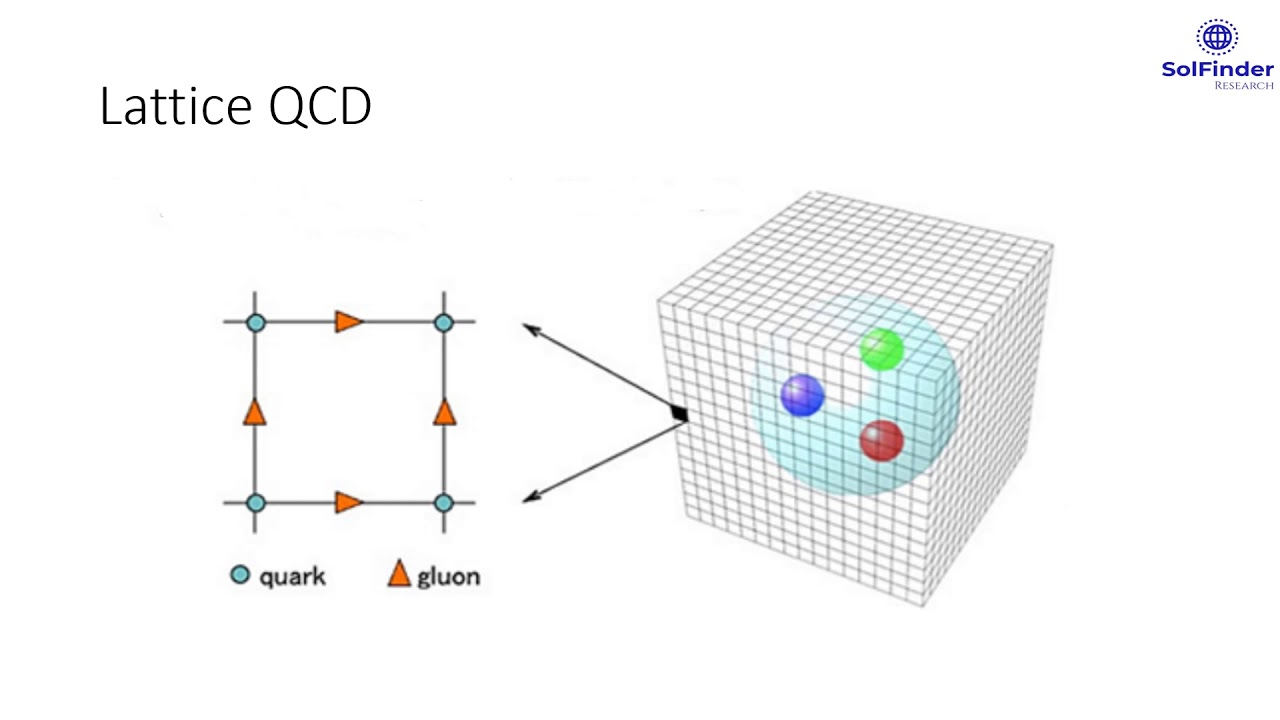
\includegraphics[width=1\textwidth]{./Images/LQCD.jpg}
% % \caption[Red LQCD]{\emph{Diagrama de una red tipo LQCD, donde los nodos representan quarks y las aristas simbolizan campos gluónicos.}}
% % \label{fig: LQCD}
% % \end{wrapfigure}

\begin{figure}[h]
    \centering
    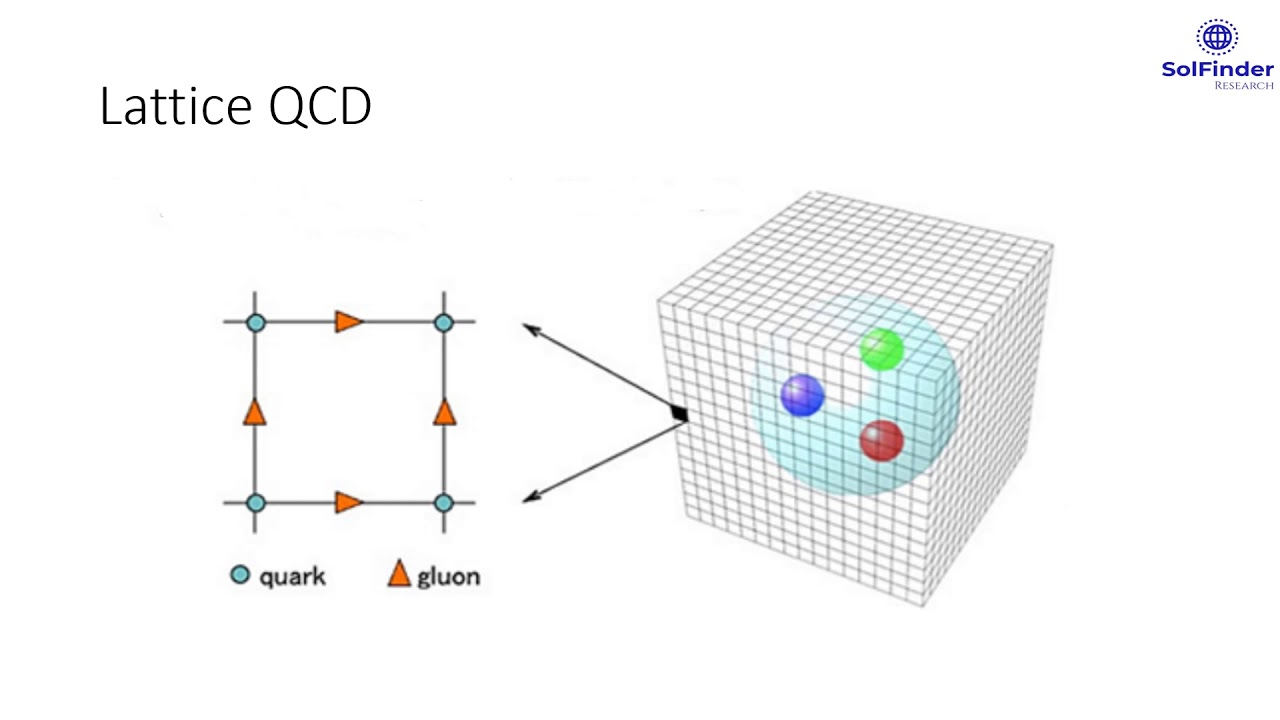
\includegraphics[width=0.8\textwidth]{./Images/LQCD.jpg}
    \caption[Red LQCD]{\emph{Diagrama de una red tipo LQCD, donde los nodos representan quarks y las aristas simbolizan campos gluónicos.} Fuente: SolFinder Research (2020).}
    \label{fig:LQCD }
\end{figure}

Diversos enfoques teóricos se han desarrollado para estudiar este confinamiento. Entre ellos destacan los modelos de cuerdas \cite{Artru1974,Andersson_1983}, los modelos de valones \cite{Hwa_1981} y los modelos de bolsa \cite{AIHPA_1968__8_2_163_0,DeTar_1983}. Este último, particularmente el \gls{bm} del \gls{mit} \cite{Chodos_1974,Chodos1974a}, ha demostrado ser eficaz en capturar propiedades globales como la masa y el radio del protón. Este modelo representa a los hadrones como cavidades esferoidales en las que los quarks libres se mueven en el interior, confinados por una presión externa (presión de bolsa) que impide su escape.

Por otro lado, técnicas numéricas como la \gls{lqcd} permiten resolver las ecuaciones de \gls{qcd} en una red discreta. Aunque altamente demandantes computacionalmente, estas simulaciones han permitido estudiar correlaciones entre hadrones y estimar parámetros de interacción. Sin embargo, enfrentan el llamado \emph{problema del signo}, que limita su aplicabilidad en ciertos regímenes \cite{Iritani_2019,Hatsuda_2017}.

La colaboración \gls{alice}, en el \gls{lhc}, ha contribuido significativamente al estudio experimental de las interacciones hadrón-hadrón, complementando cálculos teóricos con datos de correlaciones entre bariones \cite{Collaboration1984,Collaboration2020,Collaboration2021}. Estos estudios, combinados con avances en \glspl{gpd} y \glspl{gff}, han permitido acceder a cantidades como la distribución radial de presión dentro del protón \cite{Burkert_2018}.

\begin{wrapfigure}{o}{0.45\textwidth}
    \centering
    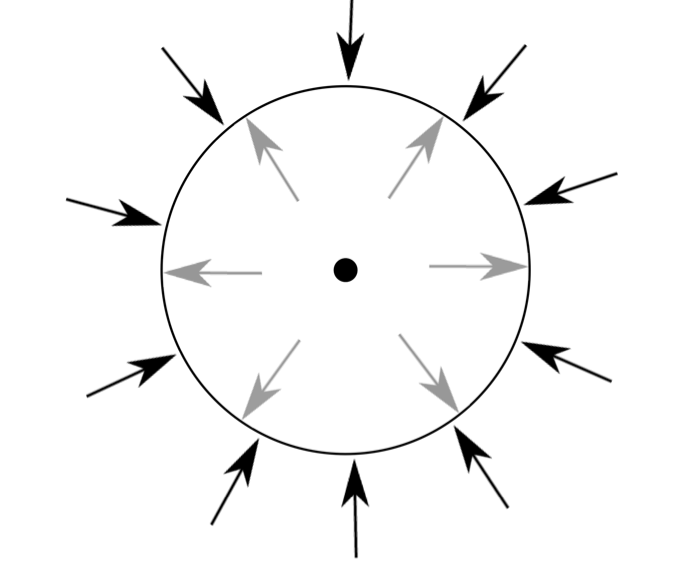
\includegraphics[width=0.4\textwidth]{./Images/Bag model.png}
    \caption[Diagrama de bolsa]{\emph{Diagrama que ilustra el modelo de bolsa. En el interior, la presión es generada por un plasma de quarks y gluones, mientras que la presión externa mantiene confinados estos componentes dentro del hadrón.} Fuente: Adaptado de The MIT bag-model Glueball mass spectrum using the MIT bag-model (2015).}
    \label{fig:Bolsa }
\end{wrapfigure}

En este contexto, modelos fenomenológicos permiten aproximar el comportamiento de los hadrones sin resolver completamente la \gls{qcd}. En esta tesis se explora una extensión del \gls{bm} mediante el uso de la estadística de \gls{tsallis}, una generalización de la estadística de \gls{bg}, ampliamente utilizada en física de altas energías para describir distribuciones de momento transversal \cite{Tsallis1988,Beck_2003,Tsallis2009,Tsallis_2009,Marques_2015}.

Esta estadística introduce un parámetro $q$ que captura desviaciones del comportamiento extensivo, lo cual podría reflejar efectos no triviales en la interacción de quarks y gluones. Su aplicación en el contexto del \gls{bm} da lugar al modelo \gls{t-mitbm}, el cual permite estudiar la distribución interna de presión y energía del protón desde una perspectiva termodinámica efectiva.

El objetivo principal de este trabajo es analizar la distribución de presión dentro del protón mediante simulaciones computacionales basadas en el modelo \gls{t-mitbm}. Se comparan los resultados obtenidos con estimaciones experimentales basadas en \gls{dvcs}\cite{Hall2018} y \gls{gpd}, y se discuten posibles interpretaciones del parámetro $q$ en este contexto.

Además, como parte de las exploraciones preliminares, se consideró la posibilidad de extender el modelo \gls{t-mitbm} para el estudio de masas hadrónicas, utilizando una reformulación de la energía interna basada en la estadística de Tsallis. Aunque este análisis permanece en una etapa inicial, abre una interesante perspectiva para futuros desarrollos del modelo, integrando cálculos de masas directamente con un tratamiento no extensivo de las energías de bolsa.

La organización del documento es la siguiente:
\begin{enumerate}[i.]
    \item En el Capítulo~\ref{ch-BagModel}, se describe el \gls{bm} y su extensión en este trabajo.
    \item En el Capítulo~\ref{ch-Tsallis}, se presenta el formalismo de la estadística de \gls{tsallis} y sus aplicaciones relevantes.
    \item En el Capítulo~\ref{ch-ProtonBagParameters}, se analiza la estructura interna del protón y se discuten resultados relevantes.
    \item En el Capítulo~\ref{ch:TotalPandGluons}, se obtiene la presion de quarks y gluones en el interior del protón y su relacion con la presion de Tsallis.
    \item En el Capítulo~\ref{ch-PhysicalMeaningQ}, se propone una interpretación física del parámetro $q$.
    \item Finalmente, el Capítulo~\ref{ch-ResultsAndConclusions} resume las conclusiones y lineamientos para trabajos futuros.
    \item Al final de los capítulos se encuentra un apéndice~\ref{app:math_derivations} con todos los desarrollos matemáticos utilizados en el trabajo.
\end{enumerate}

% Entender la estructura interna de los hadrones es fundamental para descifrar las interacciones fuertes descritas por la \gls{qcd}. Este conocimiento no solo es crucial para la física de partículas, sino que también tiene implicaciones en la comprensión de la materia en condiciones extremas, como las que existieron en los primeros momentos del universo. Según el modelo de \gls{qcd}, las partículas hadrónicas están compuestas por quarks, los cuales permanecen confinados dentro de los hadrones. Este confinamiento es una de las características fundamentales de la \gls{qcd} y explica por qué no se han observado quarks libres en la naturaleza.

% % Renombrando las figuras
% \renewcommand{\figurename}{Fig.}

% % \begin{wrapfigure}{r}{1\textwidth}
% % \centering
% % 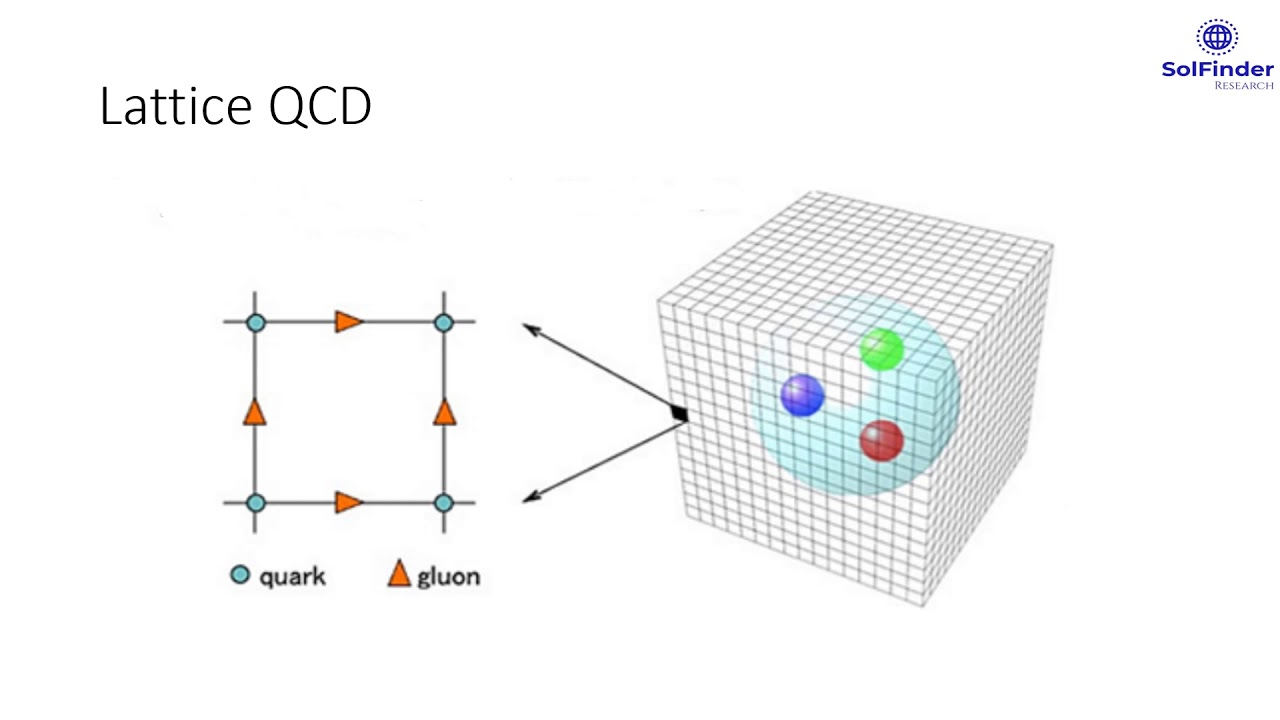
\includegraphics[width=1\textwidth]{./Images/LQCD.jpg}
% % \caption[Red LQCD]{\emph{Diagrama de una red tipo LQCD, donde los nodos representan quarks y las aristas simbolizan campos gluónicos.}}
% % \label{fig: LQCD}
% % \end{wrapfigure}

% \begin{figure}[h]
%     \centering
%     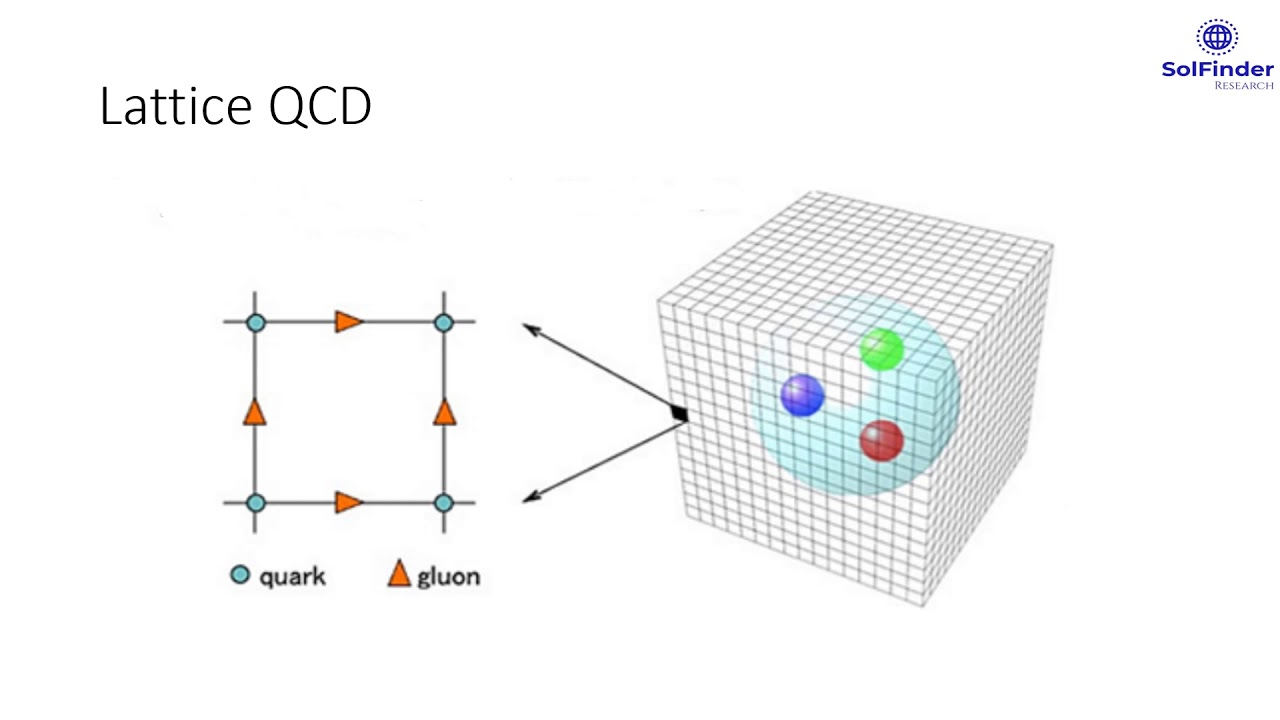
\includegraphics[width=0.8\textwidth]{./Images/LQCD.jpg}
%     \caption[Red LQCD]{\emph{Diagrama de una red tipo LQCD, donde los nodos representan quarks y las aristas simbolizan campos gluónicos.} Fuente: SolFinder Research (2020).}
%     \label{fig:LQCD }
% \end{figure}

% A lo largo de los años, se han propuesto diversos modelos fenomenológicos para describir la estructura del protón. Entre ellos destacan los modelos de cuerdas \cite{Artru1974, Andersson_1983}, que representan hadrones como cuerdas oscilantes; los modelos de bolsa \cite{AIHPA_1968__8_2_163_0,DeTar_1983}, que describen quarks confinados en una cavidad; y los modelos de valones \cite{Hwa_1981}. Cada uno de estos enfoques ofrece una perspectiva única sobre la naturaleza de los hadrones, pero todos enfrentan limitaciones al tratar de capturar la complejidad de las interacciones no lineales entre quarks y gluones.

% Para explorar la física de la materia quark, se han desarrollado técnicas avanzadas que permiten estudiar estas interacciones. Una de ellas es la \gls{lqcd}, que utiliza simulaciones numéricas en redes espacio-temporales. Sin embargo, la complejidad de estos cálculos, que involucran millones de nodos, lleva a un problema conocido como \emph{el problema del signo}. Este problema surge en simulaciones Monte Carlo, donde los pesos de las configuraciones cuánticas pueden volverse negativos o incluso complejos, imposibilitando su interpretación como probabilidades clásicas %\cite{SignProblemReference}.

% Recientemente, la colaboración \gls{hal-qcd} ha utilizado técnicas de \gls{lqcd} para realizar cálculos de vanguardia en el estudio de interacciones fuertes entre hadrones \cite{Iritani_2019,Hatsuda_2017}. Sus resultados, que describen sistemas protón-neutrón y protón-hiperón, han sido comparados con datos experimentales publicados por la colaboración \gls{alice} \cite{Collaboration2020, Collaboration2021}. Estos avances han sentado las bases para el desarrollo de modelos fenomenológicos más simples, como el que proponemos en este trabajo.

% \begin{wrapfigure}{l}{0.45\textwidth}
%     \centering
%     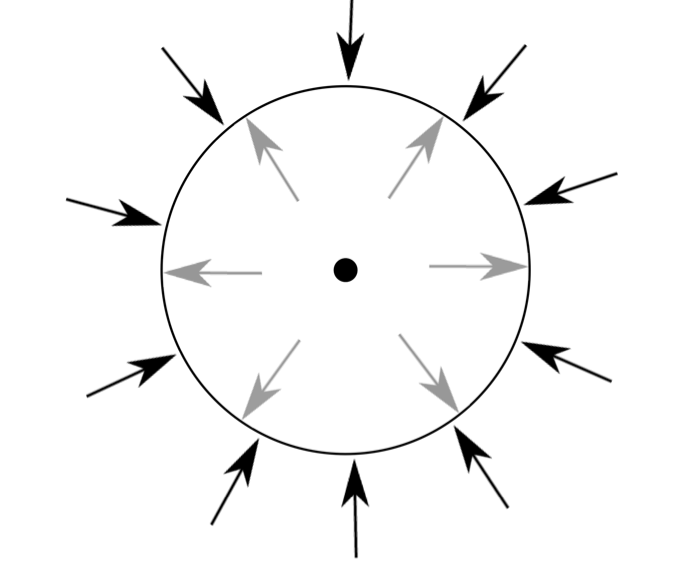
\includegraphics[width=0.4\textwidth]{./Images/Bag model.png}
%     \caption[Diagrama de bolsa]{\emph{Diagrama que ilustra el modelo de bolsa. En el interior, la presión es generada por un plasma de quarks y gluones, mientras que la presión externa mantiene confinados estos componentes dentro del hadrón.} Fuente: Adaptado de Autor (Año).}
%     \label{fig:Bolsa }
% \end{wrapfigure}

% En este trabajo, proponemos un modelo basado en el modelo de bolsa del \gls{mit} \cite{Chodos_1974,Chodos1974a} y la estadística no extensiva de \Gls{tsallis}. A este modelo lo denominamos \gls{t-mitbm}. El modelo de bolsa del \gls{mit} describe hadrones como recipientes cerrados que contienen un mar de quarks y gluones, los cuales interactúan dentro de los límites del hadrón (ver Fig.~\ref{fig:Bolsa }). Sin embargo, este modelo tradicional no captura completamente las interacciones no lineales entre quarks y gluones. Aquí es donde la estadística de \Gls{tsallis}, una generalización de la estadística de \gls{bg} \cite{Tsallis1988,Beck_2003,Tsallis2009,Tsallis_2014,Tsallis_2009}, juega un papel crucial.

% La estadística de \Gls{tsallis} introduce un parámetro $q$ que captura las interacciones entre quarks y gluones, simplificando la no linealidad inherente a estas interacciones. Este enfoque ha demostrado ser exitoso en la descripción de sistemas complejos en física de altas energías, desde colisiones electrón-positrón \cite{Bediaga_2000,Collaboration1984} hasta colisiones de iones pesados \cite{Saraswat_2018,Saraswat_2017}. En nuestro modelo, combinamos el modelo de bolsa del \gls{mit} con la estadística de \Gls{tsallis} para estimar la distribución de presión total dentro de los nucleones.

% El objetivo principal de este trabajo es proponer un modelo fenomenológico que combine el modelo de bolsa del MIT con la estadística no extensiva de \Gls{tsallis} para estudiar la distribución de presión dentro de los nucleones. Comparamos nuestros resultados con la distribución de presión de quarks obtenida recientemente mediante técnicas de \gls{dvcs} \cite{Burkert_2018}. Estas técnicas, que involucran la dispersión de fotones virtuales de altas energías, han permitido medir la presión repulsiva de los quarks cerca del centro del protón y una presión de confinamiento a distancias mayores de $0.6$.

% En los siguientes capítulos, describiremos en detalle el marco teórico del \gls{t-mitbm}, los resultados obtenidos y las comparaciones con datos experimentales. En el Capítulo \ref{ch-BagModel}, explicamos el modelo de bolsa y sus limitaciones. En el Capítulo \ref{ch-Tsallis}, presentamos la estadística no extensiva de \Gls{tsallis} y su aplicación al plasma de quarks y gluones. En el Capítulo 5, comparamos nuestros resultados con los datos experimentales de presión de quarks, y en el Capítulo 6, discutimos una posible interpretación física del parámetro de \Gls{tsallis} $q$. Finalmente, en el Capítulo 7, presentamos las conclusiones y perspectivas futuras de este trabajo.

% \newpage

% \thispagestyle{empty}
\chapter{Modelo de bolsa}
\label{ch-BagModel}

\pagestyle{fancy}
\fancyhf{}
\fancyhead[LE]{\nouppercase{\textbf{\leftmark}\hfill\textit{\rightmark}}}
\fancyhead[RO]{\nouppercase{\textit{\rightmark}\hfill\textbf{\leftmark}}}
\fancyfoot[LE]{\nouppercase{\thepage\hfill Distribución de la presión dentro de los nucleones en un modelo de bolsa de Tsallis-MIT}}
\fancyfoot[RO]{\nouppercase{Distribución de la presión dentro de los nucleones en un modelo de bolsa de Tsallis-MIT \hfill \thepage}}

\begin{chaptersummary}[Resumen del capítulo \thechapter: Modelo de bolsa]
    Este capítulo introduce el modelo de bolsa del \gls{mit} como marco fenomenológico para el confinamiento de quarks. Se parte de los fundamentos físicos provistos por la \gls{qcd} y se justifica el modelo desde la libertad asintótica, la inclusión de gluones y la estructura relativista-invariante. Se desarrolla formalmente la versión esférica del modelo, derivando sus ecuaciones de movimiento, condiciones de frontera y soluciones modales, que constituyen la base sobre la cual se construye la extensión no extensiva que proponemos más adelante.
\end{chaptersummary}
    
\section{Motivación y fundamentos desde la QCD}
    
Comprender cómo los quarks se confinan dentro de los hadrones ha sido uno de los desafíos más importantes de la física de partículas. Aunque la \gls{qcd} provee el marco teórico fundamental para describir las interacciones fuertes, su naturaleza no perturbativa a bajas energías hace difícil una solución exacta para sistemas ligados como los bariones. En este contexto, los modelos fenomenológicos como el modelo de bolsa del \gls{mit} ofrecen una herramienta útil para capturar aspectos esenciales de la dinámica hadrónica.
    
El modelo de bolsa parte de tres principios motivados por la \gls{qcd}:
    
\begin{enumerate}[a)]
\item \textbf{Confinamiento y libertad asintótica:} Los quarks están confinados a una región finita de espacio, pero se mueven libremente dentro de ella debido a la debilidad de las interacciones a corta distancia.
\item \textbf{Inclusión de gluones:} Aunque no siempre se introducen explícitamente, las correcciones debidas al intercambio de gluones son esenciales para describir propiedades del espectro hadrónico.
\item \textbf{Condición de singlete de color:} Solo estados globalmente neutros (singletes de color) son permitidos, lo cual es consistente con la ley de Gauss aplicada a campos de color confinados.
\end{enumerate}
    
A partir de estas ideas, se construye un modelo donde los quarks están confinados dentro de una “bolsa” esférica, cuyo tamaño y energía total resultan del equilibrio entre presión interna y presión de vacío externo, modelada por una constante \( B \) conocida como presión de bolsa.

\section{Formulación del modelo en cavidad esférica}

El enfoque formal del modelo parte de la acción para un campo de quarks sin masa en una cavidad esférica \cite{DeTar_1983}, dada por:

\begin{equation}
W = \int dt \left[ \int_{V} d^3x \left( \frac{i}{2} \bar{\psi} \overleftrightarrow{\partial}_{\mu} \gamma^{\mu} \psi - B \right) - \frac{1}{2} \int_{S} d^2x \bar{\psi} \psi \right]
\end{equation}

Este modelo asume:

\begin{enumerate}[i.]
\item Los quarks se comportan como partículas libres dentro de la cavidad.
\item Fuera de la cavidad, el vacío tiene menor energía, impidiendo la propagación de los campos.
\item Las condiciones de frontera imponen confinamiento y cuantizan las soluciones posibles.
\end{enumerate}

A partir de esta acción se derivan las ecuaciones de movimiento (la ecuación de Dirac) y condiciones de frontera que aseguran el confinamiento de quarks y el equilibrio de presiones. Las soluciones modales resultantes definen una base completa para construir estados hadrónicos dentro del modelo.

\section{Modelo de bolsa: descripción preliminar}

El modelo de bolsa del \gls{mit} ofrece una descripción fenomenológica del confinamiento de quarks, en la cual estos se encuentran libres en el interior de una región finita del espacio —la bolsa— y no pueden escapar debido a una presión negativa que actúa como barrera. En este esquema, los quarks se tratan como partículas relativistas sin masa dentro de la bolsa, mientras que el vacío exterior se modela como un medio con energía más baja.

Esta diferencia energética entre el interior y el exterior se modela mediante la llamada \emph{presión de bolsa} \( B \), que actúa como un parámetro fundamental para estabilizar el sistema. El tamaño de la bolsa queda entonces determinado por el equilibrio entre:

\begin{enumerate}
    \item[$\triangleright$] La \emph{energía cinética} asociada al confinamiento cuántico de los quarks,
    \item[$\triangleright$] y la \emph{energía volumétrica} proporcional a \( B \), que penaliza el crecimiento del volumen.
\end{enumerate}

Este modelo fue originalmente formulado por el grupo del MIT \cite{Chodos_1974} y ha sido extensamente utilizado para estimar propiedades de los hadrones ligeros, tales como sus masas, radios y momentos magnéticos.

\begin{wrapfigure}{l}{0.55\textwidth}
    \centering
    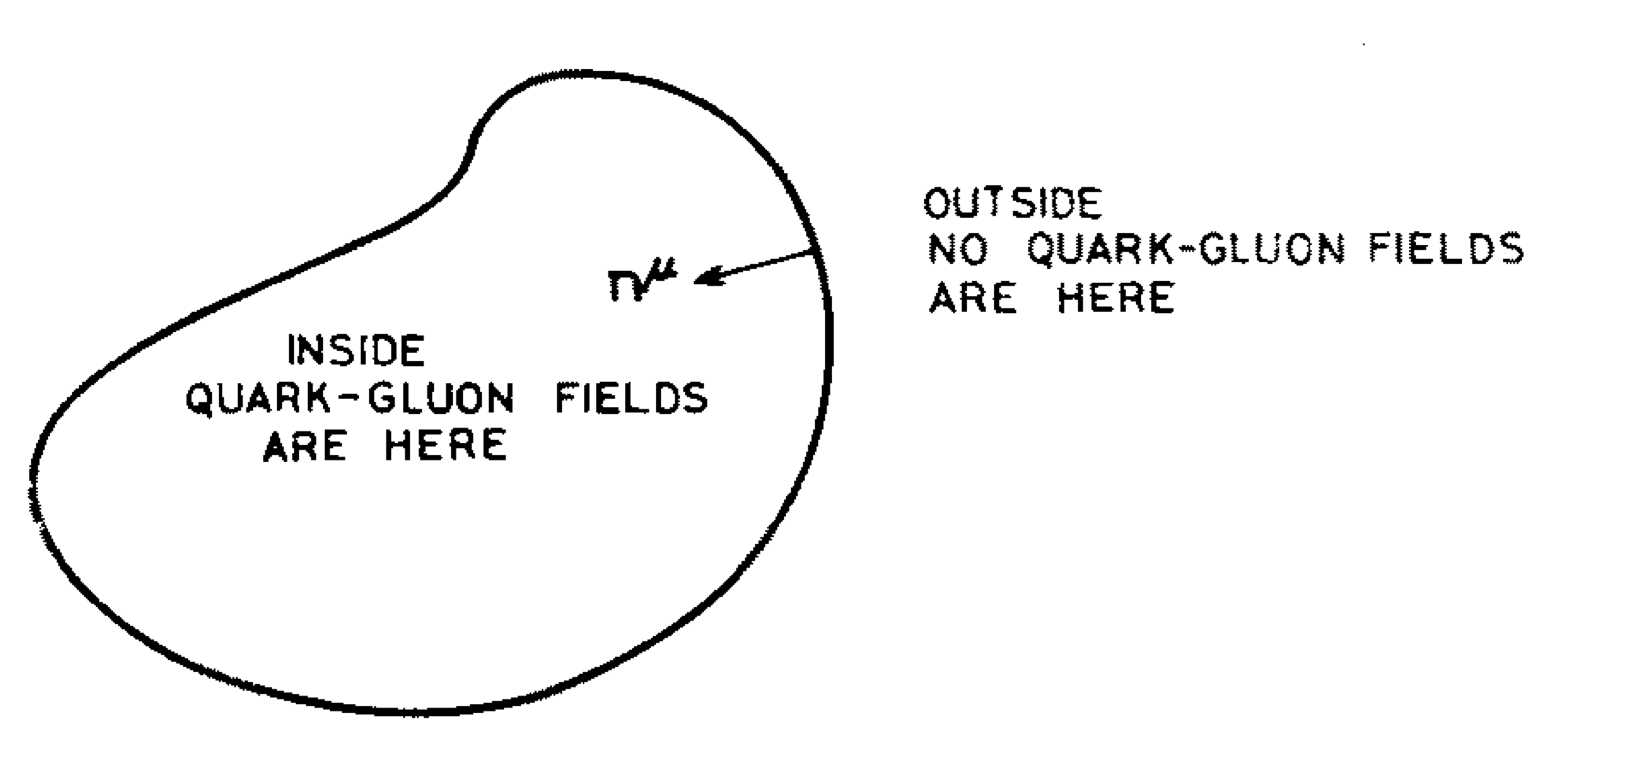
\includegraphics[width=0.5\textwidth]{./Images/Bag model BC.png}
    \caption[Modelo de bolsa con condiciones de frontera]{\emph{Dentro de la bolsa, los quarks están confinados debido a la presión de bolsa que equilibra la presión del vacío exterior.}}
    \label{fig: Bolsa BC}
\end{wrapfigure}

Desde el punto de vista de la \gls{qcd}, el modelo incorpora dos elementos fundamentales:

\begin{enumerate}[i.]
    \item \textbf{Singlete de color:} Las condiciones de frontera del modelo requieren que el estado confinado sea un singlete de color\cite{Han_1965}, en consistencia con el principio de confinamiento.
    \item \textbf{Intercambio de gluones:} Aunque el modelo en su forma más simple no incluye campos gluónicos explícitamente, se pueden incorporar como correcciones que contribuyen al espectro de energía de los estados ligados.
\end{enumerate}

A pesar de su simplicidad, el modelo ha mostrado ser efectivo al capturar ciertas características de los hadrones. En esta tesis, extendemos este marco incorporando conceptos de la estadística no extensiva de \gls{tsallis}, con el objetivo de explorar nuevas formas de describir la energía, temperatura y presión internas del protón.

\section{La aproximación de la cavidad esférica}

Una de las aproximaciones más utilizadas en el \gls{bag_model} es considerar que los quarks se encuentran confinados dentro de una región esférica de radio $R_0$, denominada \emph{cavidad esférica}. Esta simplificación permite resolver las ecuaciones del sistema bajo condiciones bien definidas, preservando los aspectos esenciales del confinamiento.

La dinámica de los quarks en esta configuración esférica se describe mediante una acción efectiva \cite{Chodos_1974}, que incluye los términos correspondientes a la energía cinética, energía de masa, presión de bolsa, y una condición de frontera:

\begin{equation} \label{eq:bag-action}
W = \int \! \mathrm{d}t \left[ \int_V \! \mathrm{d}^3x \left( \frac{i}{2} \bar{\psi} \overleftrightarrow{\partial}_{\mu} \gamma^\mu \psi - \bar{\psi} m \psi - B \right) - \frac{1}{2} \int_S \! \mathrm{d}^2x \, \bar{\psi} \psi \right],
\end{equation}

donde:
\begin{enumerate}
    \item[$\triangleright$] $\psi$ es el \emph{campo de quarks espinorial},
    \item[$\triangleright$] $B$ representa la \emph{presión de bolsa}, que actúa como energía de confinamiento,
    \item[$\triangleright$] $\bar{\psi} \overleftrightarrow{\partial}_{\mu} \gamma^\mu \psi$ es el \emph{término cinético relativista},
    \item[$\triangleright$] $m$ es la \emph{masa de los quarks} (que puede tomarse como nula en el límite relativista),
    \item[$\triangleright$] $V$ es el \emph{volumen de la bolsa} y $S$ su \emph{superficie}.
\end{enumerate}

\paragraph{Ecuaciones de movimiento:}
La ecuación de Dirac dentro de la bolsa se obtiene al variar la acción \eqref{eq:bag-action} con respecto al campo de quarks $\psi$. Esto conduce a:

\begin{equation}\label{eq-deq}
( i \slashed{\partial} - m) \psi= 0 \quad \mathrm{en} \, V,
\end{equation}

donde $\slashed{\partial} = {\partial}_{\mu} {\gamma}^{\mu}$.

\paragraph{Condiciones de frontera:}
Las condiciones de frontera en la superficie $S$ se obtienen al variar la acción \eqref{eq:bag-action} con respecto a la superficie que encierra el volumen $V$. Estas condiciones garantizan que los quarks no puedan escapar de la bolsa y que la presión externa se equilibre con la \emph{presión de bolsa} $B$:

\begin{subequations}\label{eq-bc-deq}
    \begin{empheq}[right=\empheqrbrace \quad \text{sobre} \, S \text{,}]{align}
        i {n}^{\mu} {\gamma}_{\mu} \psi &= \psi \label{eq-bc-deq-a} \\
        \frac{1}{2} {n}_{\mu} {\partial}^{\mu}(\bar{\psi} \psi) &= B \label{eq-bc-deq-b}
    \end{empheq}
\end{subequations}

\subsubsection*{Solución modal de la ecuación de Dirac}

Para resolver \eqref{eq-deq} en coordenadas esféricas, se hace uso de la separación de variables y la expansión en modos normales. La solución general adopta la forma:

\begin{equation} \label{eq:expansion-modos}
\psi(x, t) = \sum_{n\kappa jm} N(\omega_{n\kappa}) a_{n\kappa jm} \, \psi_{n\kappa jm}(x) e^{-i \omega_{n\kappa} t},
\end{equation}

donde:
\begin{enumerate}
    \item[$\triangleright$] $\omega_{n\kappa}$ son las \emph{frecuencias propias} de los modos de oscilación en la bolsa,
    \item[$\triangleright$] $N(\omega_{n\kappa})$ es una \emph{constante de normalización},
    \item[$\triangleright$] $a_{n\kappa jm}$ son \emph{coeficientes de expansión},
    \item[$\triangleright$] $\psi_{n\kappa jm}(x)$ son los \emph{modos normales}.
\end{enumerate}

Cada modo se expresa como un espinor de cuatro componentes en forma:

\begin{equation}
\psi_{n\kappa jm}(r, \theta, \phi) = 
\begin{pmatrix}
f_{n\kappa}(r) \, \Omega_{\kappa jm}(\theta,\phi) \\
i g_{n\kappa}(r) \, \Omega_{-\kappa jm}(\theta,\phi)
\end{pmatrix},
\end{equation}

donde $f_{n\kappa}(r)$ y $g_{n\kappa}(r)$ son funciones radiales obtenidas a partir de las soluciones de Bessel y $\Omega_{\kappa jm}$ son armónicos angulares con espín.

\subsection*{Condición de cuantización y frecuencias permitidas}

La condición de frontera lineal \eqref{eq-bc-deq-a} implica una relación trascendental que fija las frecuencias permitidas dentro de la bolsa \cite{Joseph1981, Chodos_1974, Lagerkvist_2015}. Esta condición se puede expresar como:

\begin{equation} \label{eq:cuantizacion}
\tan(\omega_{n\kappa}) = \frac{\omega_{n\kappa}}{\omega_{n\kappa} + \kappa}.
\end{equation}

O, de forma equivalente:

\begin{equation} \label{eq:bessel-cuanti}
j_0(\omega_{n\kappa}) = - \kappa \, j_1(\omega_{n\kappa}),
\end{equation}

donde:
\[
j_0(x) = \frac{\sin x}{x}, \quad j_1(x) = \frac{\sin x}{x^2} - \frac{\cos x}{x}.
\]

Las primeras raíces de estas ecuaciones determinan los valores discretos de $\omega_{n\kappa}$ que caracterizan los estados cuánticos permitidos. Algunos de los primeros valores son:

\[
\begin{array}{ccc}
\kappa = -1: & \omega_{1,-1} \approx 2.04, & \omega_{2,-1} \approx 5.40 \\
\kappa = +1: & \omega_{1,1} \approx 3.81, & \omega_{2,1} \approx 7.00
\end{array}
\]


\begin{remark}[Sobre los modos espinoriales]
    Para los estados de espín \( j = \frac{1}{2} \), que corresponden a los quarks constituyentes de los hadrones, las soluciones a la ecuación de Dirac bajo las condiciones de frontera \eqref{eq-bc-deq} presentan dos configuraciones relevantes: \( \kappa = \pm 1 \). Estas soluciones modales involucran funciones de Bessel esféricas y espinores angulares, y permiten describir cuantitativamente el comportamiento energético del sistema.

    \paragraph{Soluciones específicas para \( j = \frac{1}{2} \):}
    
    \begin{itemize}
    \item Para \( \kappa = -1 \):
    \begin{equation}
    \psi_{n, -1, \frac{1}{2}, m}(x,t) = \frac{1}{\sqrt{4\pi}} 
    \begin{pmatrix}
    i j_0\left( \frac{\omega_{n,-1} r}{R_0} \right) U_m \\
    - j_1\left( \frac{\omega_{n,-1} r}{R_0} \right) \sigma \cdot \hat{r} \, U_m
    \end{pmatrix}
    e^{-i \omega_{n,-1} t / R_0}
    \end{equation}
    
    \item Para \( \kappa = 1 \):
    \begin{equation}
    \psi_{n, 1, \frac{1}{2}, m}(x,t) = \frac{1}{\sqrt{4\pi}} 
    \begin{pmatrix}
    i j_1\left( \frac{\omega_{n,1} r}{R_0} \right) \sigma \cdot \hat{r} \, U_m \\
    j_0\left( \frac{\omega_{n,1} r}{R_0} \right) U_m
    \end{pmatrix}
    e^{-i \omega_{n,1} t / R_0}
    \end{equation}
    \end{itemize}
    
    donde \( U_m \) es un espinor de Pauli y \( j_\ell(z) \) son las funciones de Bessel esféricas:
    \[
    j_0(x) = \frac{\sin x}{x}, \quad j_1(x) = \frac{\sin x}{x^2} - \frac{\cos x}{x}.
    \]
    
    
    Aunque en este trabajo no se hace uso directo de estas soluciones específicas, su estructura y cuantización son fundamentales para posibles estudios futuros que busquen determinar las masas hadrónicas a partir de la contribución energética de los modos confinados. Esta dirección será brevemente comentada en el capítulo de conclusiones.
\end{remark}

\subsection*{Resultados físicos del modelo}

El modelo permite derivar relaciones relevantes para sistemas hadrónicos. En particular:

\begin{enumerate}[a)]
    \item La energía total de la bolsa es proporcional al volumen promediado:  
    \[
    E = 4B \langle V \rangle.
    \]
    
    \item En el límite termodinámico, el sistema tiene una temperatura característica \( T_0 \sim B^{-1/4} \) (esto se verá en el capítulo \ref{ch-ProtonBagParameters}), independiente de su energía total. Esto implica una densidad de estados de tipo exponencial:
    \[
    \zeta(E) \sim e^{E/T_0}.
    \]
\end{enumerate}

\blankpage
\chapter{Presión de quarks y gluones en el marco de la estadística de Tsallis}\label{ch-Tsallis}

% \pagestyle{fancy}
% \fancyhead{} % clear all header fields
% \fancyhead[RO,LE]{\textbf{\chaptername\,\thechapter}  }
% \fancyfoot{} % clear all footer fields
% \fancyfoot[LE,RO]{\thepage}
% % \fancyfoot[LO,CE]{Introducción}
% \fancyfoot[CO,CE]{Estadística de Tsallis}

% =====================Estilo de página================================
\pagestyle{fancy}
\fancyhf{} % Limpia todos los campos de encabezado y pie de página
\fancyhead[LE]{\nouppercase{\textit{\rightmark}}} % Sección en páginas pares (izquierda)
\fancyhead[RO]{\nouppercase{\textit{\rightmark}}} % Sección en páginas impares (derecha)
\fancyhead[RE]{\nouppercase{\hfill \textbf{Capítulo 2. Presión de quarks y gluones en\\el marco de la estadística de Tsallis}}} % Capítulo en páginas impares (izquierda)
\fancyhead[LO]{\nouppercase{\textbf{Capítulo 2. Presión de quarks y gluones en\\el marco de la estadística de Tsallis} \hfill}} % Capítulo en páginas pares (derecha)
\fancyfoot[LE]{\nouppercase{\thepage \hfill {Distribución de la presión dentro de los nucleones en un modelo de bolsa de Tsallis-MIT}}} % Pie de página en páginas pares
\fancyfoot[RO]{\nouppercase{{Distribución de la presión dentro de los nucleones en un modelo de bolsa de Tsallis-MIT} \hfill \thepage}} % Pie de página en páginas impares
% =====================================================================

\begin{chaptersummary}[Resumen del capítulo \thechapter: Estadística de Tsallis]
    En este capítulo se introduce el marco teórico de la estadística no extensiva de Tsallis, una generalización de la estadística de Boltzmann-Gibbs. Se presentan las definiciones fundamentales de entropía, energía interna y temperatura en el formalismo \( q \)-generalizado, así como su relación con las funciones de partición y distribuciones de probabilidad. 
\end{chaptersummary}

%%%%%%%%%%%%%%%%%%%%%%%%%%%%%%%%%%%%%%%%%%%%%%%%%%%%%%%%%%%%%%%%%%%%%%%%%%%%%%%%%%%%%%%%%%%%%%%%%%%%%%%%%%%%%
\section{Fundamentos de la estadística de Tsallis}

La estadística no extensiva de Tsallis fue propuesta en 1988 como una generalización del marco tradicional de Boltzmann-Gibbs, con el objetivo de describir sistemas complejos que exhiben correlaciones de largo alcance, inestabilidad caótica o estructuras no ergódicas \cite{Tsallis1988, Tsallis2009, Tsallis_2009}.

El enfoque de Tsallis introduce un parámetro de no extensividad \( q \in \mathbb{R} \), a partir del cual se define una entropía generalizada:

\begin{equation}
    S_q = k_{\mathrm{B}} \frac{1 - \sum_i p_i^q}{q - 1},
\end{equation}

donde \( p_i \) representa la probabilidad del microestado \( i \), y \( k_{\mathrm{B}} \) es la constante de Boltzmann. En el límite \( q \rightarrow 1 \), se recupera la entropía de Boltzmann-Gibbs:

\begin{equation}
    \lim_{q \rightarrow 1} S_q = -k_{\mathrm{B}} \sum_i p_i \ln p_i.
\end{equation}

Este formalismo ha demostrado ser exitoso en la descripción de sistemas como plasmas astrofísicos, turbulencia, colisiones hadrónicas y materia nuclear, donde las distribuciones de energía no presentan un decaimiento exponencial, sino colas de potencia que reflejan una dinámica fuera del equilibrio termodinámico \cite{Tsallis_2014, Barboza_Mendoza_2019, Bhattacharyya_2018}.

\break

Bajo esta generalización, en un sistema constituido por dos subsistemas probabilisticamente independientes $A$ y $B$ (i.e., si ${p}_{ij}^{A+B} = {p}_{i}^{A}{p}_{j}^{B}$), entonces 

\begin{equation}\label{eq-TsallisTwoSystems}
\frac{{S}_{{q}}(A+B)}{{k}_{\mathrm{B}}} = \frac{{S}_{q}(A)}{{k}_{\mathrm{B}}} + \frac{{S}_{q}(B)}{{k}_{\mathrm{B}}} + (1 - q) \frac{{S}_{q}(A)}{{k}_{\mathrm{B}}}\frac{{S}_{q}(B)}{{k}_{\mathrm{B}}}\footnote{Más adelante se usarán unidades naturales por lo que no aparecerá la constante de Boltzmann, ${k}_{\mathrm{B}}$},
\end{equation}

de donde se observa claramente que cuando $q=1$ se regresa a la estadística de \gls{bg} 

En este capítulo, emplearemos esta generalización para explorar la termodinámica de un sistema de quarks y gluones confinado, extendiendo el modelo de bolsa del MIT mediante distribuciones \( q \)-generalizadas, lo cual permitirá caracterizar presiones internas y densidades de energía con mayor generalidad.

%%%%%%%%%%%%%%%%%%%%%%%%%%%%%%%%%%%%%%%%%%%%%%%%%%%%%%%%%%%%%%%%%%%%%%%%%%%%%%%%%%%%%%%%%%%%%%%%%%%%%%%%%%%%%
\section{Presión dentro del hadrón}
\label{sec-PresTsa}

A partir de la ecuación \eqref{eq-TsallisTwoSystems}, es posible obtener la entropía y presión dentro de un hadrón considerado como una mezcla de gases de quarks y gluones\ \cite{Greiner2001}. Para ello, analizamos por separado las contribuciones de cada componente, asumiendo que:

\begin{enumerate}[i.]
    \item Los \emph{quarks} se comportan como un gas ideal ultrarrelativista de Fermi-Dirac sin masa.
    \item Los \emph{gluones} se modelan como un gas ideal ultrarrelativista de Bose-Einstein, también sin masa.
\end{enumerate}

Ambos gases se consideran libres y no interactuantes de forma explícita, ya que la interacción efectiva se introduce mediante el parámetro de no extensividad \( q \) de Tsallis.

% ------------------------------------------------------------------------------------------------ %
\subsection{Presión de gluones: gas ideal ultrarrelativista de Bose-Einstein}

Los niveles de energía de los gluones, como bosones sin masa, se describen por:

\begin{equation}
\epsilon_k = c p = \hbar c k,
\end{equation}

donde \( p \) es el momento y \( k \) el número de onda del modo. La función de partición canónica para este sistema es:

\begin{equation}\label{eq-partfunc}
\Xi^{\mathrm{BE}}(T,V,\mu) = \prod_j \frac{1}{1 - \xi e^{-\beta \epsilon_j}},
\end{equation}

con \( \beta = ({k}_{\mathrm{B}} T)^{-1} \) y fugacidad \( \xi = e^{\beta \mu} \). El número promedio de partículas por estado es:

\begin{equation}
\langle n_j \rangle = \frac{1}{\xi^{-1} e^{\beta \epsilon_j} - 1}.
\end{equation}

Las cantidades termodinámicas fundamentales se obtienen sumando sobre todos los estados:

\begin{align}
N(T,V,\mu) &= \sum_j \langle n_j \rangle = \sum_j \frac{1}{\xi^{-1} e^{\beta \epsilon_j} - 1}, \label{eq-BE-Ntotal} \\
E(T,V,\mu) &= \sum_j \epsilon_j \langle n_j \rangle = \sum_j \frac{\epsilon_j}{\xi^{-1} e^{\beta \epsilon_j} - 1}. \label{eq-BE-Etotal}
\end{align}

\break

En el límite termodinámico, estas sumas se reemplazan por integrales utilizando la densidad de estados:

\begin{equation}
\Sigma(\epsilon) \, d\epsilon = \frac{4\pi V}{(hc)^3} \epsilon^2 d\epsilon,
\end{equation}

lo que permite reescribir:

\begin{align}
{N}_{G}(T,V,\mu) &= \frac{4\pi V}{(hc)^3} \int_0^\infty \frac{\epsilon^2 \, d\epsilon}{\xi^{-1} e^{\beta \epsilon} - 1}, \label{eq-BE-Ntotalint} \\
{E}_{G}(T,V,\mu) &= \frac{4\pi V}{(hc)^3} \int_0^\infty \frac{\epsilon^3 \, d\epsilon}{\xi^{-1} e^{\beta \epsilon} - 1}. \label{eq-BE-Etotalint}
\end{align}

En el caso particular de los gluones, se tiene \( \mu = 0 \), ya que su número no está conservado, y la fugacidad se vuelve \( \xi = 1 \). Las expresiones anteriores se simplifican a:

\begin{align}
{N}_{G}(T,V) &= \frac{4\pi V}{(hc)^3} \int_0^\infty \frac{\epsilon^2 \, d\epsilon}{e^{\beta \epsilon} - 1}, \label{eq-BE-Ntotalintnofug} \\
{E}_{G}(T,V) &= \frac{4\pi V}{(hc)^3} \int_0^\infty \frac{\epsilon^3 \, d\epsilon}{e^{\beta \epsilon} - 1}. \label{eq-BE-Etotalintnofug}
\end{align}

Mediante el cambio de variable \( x = \beta \epsilon \), estas integrales toman la forma:

\begin{align}
{N}_{G}(T,V) &= \frac{4\pi V}{(hc)^3 \beta^3} \int_0^\infty \frac{x^2 dx}{e^x - 1}, \label{eq-BE-Ntotalintnofug-x} \\
{E}_{G}(T,V) &= \frac{4\pi V}{(hc)^3 \beta^4} \int_0^\infty \frac{x^3 dx}{e^x - 1}. \label{eq-BE-Etotalintnofug-x}
\end{align}

Estas integrales se evalúan con funciones especiales:

\begin{align}
\int_0^\infty \frac{x^2 dx}{e^x - 1} &= \Gamma(3)\zeta(3) = 2\zeta(3), \label{eq-sol-int-N} \\
\int_0^\infty \frac{x^3 dx}{e^x - 1} &= \Gamma(4)\zeta(4) = \frac{\pi^4}{15}. \label{eq-sol-int-E}
\end{align}

Finalmente, considerando la degeneración de gluones \( g_G = 16 \) (8 tipos de gluones con 2 polarizaciones), y trabajando en unidades naturales \( \hbar = c = {k}_{\mathrm{B}} = 1 \), obtenemos:

\begin{equation}\label{eq-BE-Etotalgluons}
E_G = g_G \frac{\pi^2}{30} V T^4,
\end{equation}

\begin{equation}\label{eq-BE-Pgluons}
P_G = \frac{1}{3} \frac{E_G}{V} = g_G \frac{\pi^2}{90} T^4.
\end{equation}

La entropía asociada al sistema de gluones se expresa como:

\begin{equation}\label{eq-BE-Sgluons}
S_G = \frac{4}{3} \frac{E_G}{T} = g_G \frac{4\pi^2}{90} V T^3.
\end{equation}

% ------------------------------------------------------------------------------------------------ %
\subsection{Presión de quarks: gas ideal ultrarrelativista de Fermi-Dirac}
\label{sec-Pquarks}

Consideramos ahora la contribución de los quarks y antiquarks, modelados como un sistema mixto de fermiones sin masa en el régimen ultrarrelativista. Bajo esta aproximación, la energía de una partícula se reduce a \( \epsilon = |\vec{p}| c \)\footnote{Resultado obtenido al tomar el límite \( m \to 0 \) en la relación relativista \( \epsilon = \sqrt{p^2 c^2 + m^2 c^4} \).}.

\paragraph{Características del sistema:}
\begin{itemize}
    \item[$\triangleright$] Se trata de un gas compuesto por quarks y antiquarks en equilibrio termodinámico.
    \item[$\triangleright$] Se impone simetría entre partículas y antipartículas: \( \mu_+ = -\mu_- = \mu \).
    \item[$\triangleright$] Factor de degeneración: \( g_Q = 12 \) (2 espines × 3 colores × 2 sabores \( u,d \)).
\end{itemize}

% .-.-.-.-.-.-.-.-.-.-.-.-.-.-.-.-.-.-.-.-.-.-..-.-.-.-.-.-.-.-.-.-.-.-.-.-.-.-.-.-.-.-.-.-.-.-.-.-.%

\subsubsection*{Función de partición}

La función de partición total para el sistema combinado es el producto de las funciones de quarks y antiquarks:

\begin{equation}
\Xi(T, V, \mu) = \prod_j \left(1 + e^{-\beta(\epsilon_j - \mu)}\right)
\prod_j \left(1 + e^{-\beta(\epsilon_j + \mu)}\right),
\end{equation}

donde el índice \( j \) recorre todos los estados energéticos posibles.

% .-.-.-.-.-.-.-.-.-.-.-.-.-.-.-.-.-.-.-.-.-.-..-.-.-.-.-.-.-.-.-.-.-.-.-.-.-.-.-.-.-.-.-.-.-.-.-.-.%

\subsubsection*{Número de partículas y exceso neto}

La población media de partículas en cada estado se expresa como:

\begin{equation}
N_\pm = \sum_j \frac{1}{e^{\beta(\epsilon_j \mp \mu)} + 1},
\end{equation}

y el número neto de quarks (exceso sobre antiquarks) es:

\begin{equation}\label{eq-FD-Excedente}
{N}_{Q} = N_+ - N_- = \frac{g_Q V}{6 \pi^2} \left( \pi^2 \mu T^2 + \mu^3 \right),
\end{equation}

resultado obtenido tras pasar al límite termodinámico e integrar sobre la densidad de estados.

% .-.-.-.-.-.-.-.-.-.-.-.-.-.-.-.-.-.-.-.-.-.-..-.-.-.-.-.-.-.-.-.-.-.-.-.-.-.-.-.-.-.-.-.-.-.-.-.-.%

\subsubsection*{Energía total y presión}

La energía total se calcula a partir de la suma de contribuciones energéticas de quarks y antiquarks:

\begin{equation}\label{eq-FD-Energy}
E_Q = g_Q V T^4 \left[
\frac{7 \pi^2}{120} + \frac{1}{4} \left( \frac{\mu}{T} \right)^2 + \frac{1}{8 \pi^2} \left( \frac{\mu}{T} \right)^4
\right].
\end{equation}

Dado que se trata de un gas ultrarrelativista, la presión asociada satisface \( P_Q = E_Q / (3V) \), por lo que:

\begin{equation}
P_Q = \frac{g_Q T^4}{3} \left[
\frac{7 \pi^2}{120} + \frac{\mu^2}{4 T^2} + \frac{\mu^4}{8 \pi^2 T^4}
\right].
\end{equation}

% .-.-.-.-.-.-.-.-.-.-.-.-.-.-.-.-.-.-.-.-.-.-..-.-.-.-.-.-.-.-.-.-.-.-.-.-.-.-.-.-.-.-.-.-.-.-.-.-.%

\subsubsection*{Entropía}

Aplicando la relación termodinámica:

\[
S = \frac{{E}_{Q} + P V - \mu {N}_{Q}}{T},
\]

se obtiene la entropía total del sistema:

\begin{equation}\label{eq-FD-Entropy}
S_Q = g_Q V T^3 \left[
\frac{7 \pi^2}{90} + \frac{1}{6} \left( \frac{\mu}{T} \right)^2
\right].
\end{equation}

\paragraph{Nota:} Las derivaciones completas de estas expresiones pueden consultarse en el Apéndice~\ref{app:math_derivations}.


\section{El protón en el modelo de Tsallis}
\label{sec-proton-tsallis}

Una vez obtenidas las propiedades termodinámicas de los gases de gluones y quarks en el marco de la estadística de Boltzmann-Gibbs (BG), es posible extender este análisis al contexto de la estadística de Tsallis, considerando al protón como un sistema compuesto por ambos componentes correlacionados.

\paragraph{Configuración del sistema}

El modelo no extensivo considera al protón como una mezcla compuesta por:

\begin{enumerate}[i.]
    \item Un gas de quarks y antiquarks sin masa, regido por la estadística de Fermi-Dirac.
    \item Un gas de gluones, bosones sin masa, obedeciendo estadística de Bose-Einstein.
\end{enumerate}

Ambos sistemas se consideran independientes a nivel de estado, pero correlacionados globalmente mediante una formulación no extensiva.

\subsection{Entropía generalizada de Tsallis}

La entropía total del sistema se describe mediante la expresión de Tsallis para dos subsistemas independientes \( A \) y \( B \):

\begin{equation}
S_q(A+B) = S_q(A) + S_q(B) + (1 - q) S_q(A) S_q(B),
\end{equation}

donde \( q \in \mathbb{R} \) es el parámetro de no extensividad. Aplicado al sistema hadrónico:

\begin{equation}\label{eq-Entropy-Tsallis}
S_q = S_1(Q) + S_1(G) + (1 - q) S_1(Q) S_1(G),
\end{equation}

donde \( S_1(Q) \) y \( S_1(G) \) son las entropías de quarks y gluones calculadas bajo la estadística estándar de Boltzmann-Gibbs.

\paragraph{Interpretación física del parámetro \( q \):}
\begin{itemize}
    \item[$\triangleright$] \( q = 1 \): Recupera la estadística extensiva estándar.
    \item[$\triangleright$] \( q > 1 \): Describe correlaciones negativas (efectos de exclusión o repulsión).
    \item[$\triangleright$] \( q < 1 \): Describe correlaciones positivas (agrupamiento o efectos de atracción).
\end{itemize}

Este parámetro ha sido empleado exitosamente para describir sistemas como plasmas cuánticos, colisiones hadrónicas y materia nuclear a altas energías \cite{Tsallis_2014, Bhattacharyya_2018, Barboza_Mendoza_2019}.

\subsubsection*{Límite extensivo \( q \to 1 \)}

En el caso límite de \( q = 1 \), la expresión \eqref{eq-Entropy-Tsallis} se reduce a:

\begin{equation}\label{eq-BG-limit}
S_{q \to 1} = S_{Q+G} = S_1(Q) + S_1(G),
\end{equation}

cuyas formas explícitas, con degeneraciones \( g_Q = 12 \), \( g_G = 16 \), son:

\begin{align}
S_1(Q) &= g_Q V T^3 \left[ \frac{7 \pi^2}{90} + \frac{1}{6} \left( \frac{\mu}{T} \right)^2 \right], \\
S_1(G) &= g_G V T^3 \frac{4 \pi^2}{90}.
\end{align}

\subsubsection*{Forma explícita general para \( S_q \)}

Sustituyendo en \eqref{eq-Entropy-Tsallis}:

\begin{equation}\label{eq-Tsallis-Entropy-final}
\begin{split}
S_q &= \left[ \frac{74 \pi^2}{45} + 2 \left( \frac{\mu}{T} \right)^2 \right] V T^3 \\
&\quad + \frac{128 \pi^2}{15} (1 - q) \left[ \frac{7 \pi^2}{90} + \frac{1}{6} \left( \frac{\mu}{T} \right)^2 \right] V^2 T^6,
\end{split}
\end{equation}

donde el primer término corresponde a la suma extensiva y el segundo a la corrección cuadrática en volumen derivada de las correlaciones no extensivas.

\subsection{Presión generalizada en el marco de Tsallis}
\label{subsec-Tsallis-pressure}

Aplicando la relación termodinámica de Maxwell para sistemas con entropía generalizada:

\begin{equation}\label{eq-Maxwell-Tsallis}
\left( \frac{\partial S_q}{\partial V} \right)_{T, \mu} = \left( \frac{\partial P_q}{\partial T} \right)_{V, \mu},
\end{equation}

y considerando la forma explícita de \( S_q \) obtenida en \eqref{eq-Tsallis-Entropy-final}, se obtiene (ver derivación completa en el Apéndice \ref{app:Tsallis-pressure}):

\begin{equation}\label{eq-Pq-final}
\begin{split}
P_q &= \underbrace{T^4 \left[ \frac{37 \pi^2}{90} + \left( \frac{\mu}{T} \right)^2 + \frac{1}{2 \pi^2} \left( \frac{\mu}{T} \right)^4 \right]}_{\text{Componente extensiva}} \\
&\quad + \underbrace{\frac{256 \pi^2}{15} (1 - q) V T^7 \left[ \frac{\pi^2}{90} + \frac{1}{30} \left( \frac{\mu}{T} \right)^2 \right]}_{\text{Corrección no extensiva}}.
\end{split}
\end{equation}

\paragraph{Análisis de los términos:}
\begin{itemize}
    \item El término \( \sim T^4 \) es la presión total bajo estadística BG.
    \item La corrección \( \sim V T^7 (1-q) \) revela el impacto de las correlaciones no extensivas, particularmente dominante a altas temperaturas.
    \item Se preserva la simetría \( \mu \leftrightarrow -\mu \).
\end{itemize}

\subsubsection*{Comparación entre estadística BG y Tsallis}

\begin{table}[h]
    \centering
    \caption{Comparación entre resultados termodinámicos en BG y Tsallis}
    \begin{tabular}{lcc}
        \toprule
        \textbf{Propiedad} & \textbf{BG (\( q = 1 \))} & \textbf{Tsallis (\( q \neq 1 \))} \\
        \midrule
        Entropía & Aditiva & No aditiva (correlaciones) \\
        Presión & \( \sim T^4 \) & \( \sim T^4 + (1 - q) V T^7 \) \\
        \bottomrule
    \end{tabular}
    \label{tab:BG-vs-Tsallis}
\end{table}


\begin{figure}[!h]
    \centering
    \begin{tikzpicture}[
        node distance=1.5cm,
        concept/.style={rectangle, draw, rounded corners=3pt, fill=blue!10, minimum width=4cm, text width=3.8cm, align=center},
        interaction/.style={ellipse, draw, fill=green!20, minimum width=3cm, align=center},
        result/.style={rectangle, draw, fill=red!10, minimum width=4cm, text width=3.8cm, align=center},
        arrow/.style={->, >=stealth, thick},
        dashedarrow/.style={->, >=stealth, thick, dashed}
    ]
    
    % Nodos principales
    \node[concept] (q) {Parámetro de Tsallis \\ $q$};
    \node[interaction, below left=2cm and 0.5cm of q] (interpretation) {
        \textbf{Interpretación:} \\
        $q=1$: BG estándar \\
        $q>1$: Correlaciones negativas \\
        $q<1$: Correlaciones positivas
    };
    \node[concept, below right=2cm and 0.5cm of q] (entropy) {
        \textbf{Entropía no extensiva} \\
        $S_q = S_1(Q) + S_1(G)$ \\
        $+ (1-q)S_1(Q)S_1(G)$
    };
    \node[result, below=2cm of entropy] (pressure) {
        \textbf{Presión generalizada} \\
        $P_q = P_{\text{BG}}$ \\
        $+ \frac{256\pi^2}{15}(1-q)V T^7$
    };
    
    % Conexiones principales
    \draw[arrow] (q) -- node[left, near start] {Controla} (entropy);
    \draw[arrow] (entropy) -- node[right] {Determina} (pressure);
    
    % Conexiones de interpretación (ajustadas)
    \draw[dashedarrow] (q) -- node[above, sloped, pos=0.6] {Describe} (interpretation.north);
    \draw[dashedarrow] (interpretation.east) -- ++(0.5,0) |- node[pos=0.55, above] {Afecta} (entropy.west);
    
    % Leyenda explicativa reposicionada
    \node[below=0.8cm of interpretation, text width=5cm, align=left, font=\small] {
        \textbf{Relaciones físicas:} \\
        \begin{enumerate}
            \item[$\triangleright$] El parámetro $q$ modifica la entropía
            \item[$\triangleright$] La entropía generalizada afecta la presión
            \item[$\triangleright$] Todo converge a BG cuando $q=1$
        \end{enumerate}
    };
    \end{tikzpicture}
    \caption[Diagrama de relaciones Tsallis]{Jerarquía de relaciones en el modelo: (1) El parámetro $q$ controla la entropía no extensiva $S_q$; (2) Las interpretaciones físicas de $q$ (caja verde) justifican su uso; (3) La entropía modificada determina la presión generalizada $P_q$. Las flechas punteadas indican relaciones secundarias.}
    \label{fig:Tsallis-flow-complete}
\end{figure}

Como muestra la Figura \ref{fig:Tsallis-flow-complete}, el parámetro $q$ no solo controla la entropía del sistema (Ec. \ref{eq-Entropy-Tsallis}), sino que a través de su interpretación como medidor de correlaciones (recuadro verde), afecta directamente las propiedades termodinámicas como la presión (Ec. \ref{eq-Pq-final}).

\begin{remark}[Relevancia física del parámetro \( q \)]
El parámetro \( q \) funciona como cuantificador de correlaciones a largo alcance, acoplamientos residuales o desviaciones del equilibrio térmico. Su valor en sistemas de QCD típicamente se encuentra en el rango \( q \approx 1.1 - 1.2 \), según se ha observado en colisiones hadrónicas y sistemas de materia nuclear \cite{Bhattacharyya_2018, Tsallis_2014}.
\end{remark}


\section*{Conclusiones del capítulo}
Este capítulo ha establecido una base termodinámica sólida para describir la presión y la entropía en sistemas de quarks y gluones mediante el formalismo no extensivo de Tsallis. La generalización obtenida permite capturar efectos de correlación entre los constituyentes, que serán explorados más adelante en contextos fenomenológicos o comparaciones con datos experimentales.

\blankpage
\chapter{Parámetros Característicos del Protón en el Modelo de Bolsa}\label{ch-ProtonBagParameters}

\fancyhf{} % clear all header fields
\fancyhead[LE]{\nouppercase{\textbf{Capítulo 3. Características de estructura \\del protón}\hfill\textit{\rightmark}}}
\fancyhead[RO]{\nouppercase{\textit{\rightmark}\hfill\textbf{Capítulo 3. Características de estructura \\del protón}}}
\fancyfoot[LE]{\nouppercase{\thepage\hfill {Distribución de la presión dentro de los nucleones en un modelo de bolsa de Tsallis-MIT}}}
\fancyfoot[RO]{\nouppercase{{Distribución de la presión dentro de los nucleones en un modelo de bolsa de Tsallis-MIT} \hfill \thepage}}

\begin{chaptersummary}[Resumen del capítulo \thechapter: Parámetros del protón en el modelo de bolsa]
    Este capítulo establece los parámetros fundamentales del protón derivados del modelo de bolsa MIT, analizando dos configuraciones gluónicas: 1) quarks inmersos en un mar de gluones y 2) quarks rodeados por un cascarón gluónico. Se determinan los perfiles radiales de temperatura y presión de bolsa, sentando las bases para el cálculo de la distribución completa de presión en el siguiente capítulo.
\end{chaptersummary}

\begin{wrapfigure}{r}{0.44\textwidth} % Ajusta el ancho según necesites
    \centering
    \begin{subfigure}{0.2\textwidth} % Reduje el ancho para dejar espacio al margen
        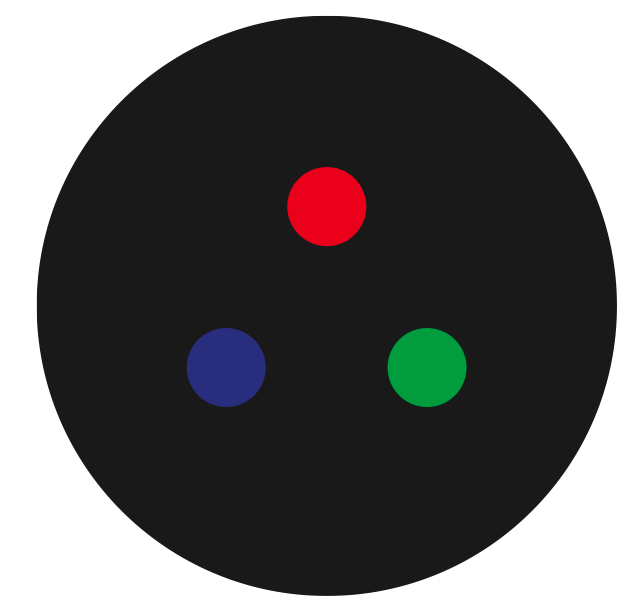
\includegraphics[width=\linewidth]{./Images/Bag_model_sea_cropped.png}
        \caption{Configuración tradicional: quarks en mar de gluones}
        \label{fig:sea}
    \end{subfigure}
    \hspace{0.1cm} % Espacio vertical entre subfiguras
    \begin{subfigure}{0.21\textwidth}
        
\includegraphics[width=\linewidth]{./Images/Bag_model_shell_cropped.png}
        \caption{Configuración propuesta: gluones como cascarón confinante}
        \label{fig:shell}
    \end{subfigure}
    \caption[Configuraciones gluónicas del modelo de bolsa]{Configuraciones gluónicas. \textbf{(a)} Quarks en mar de gluones; \textbf{(b)} Quarks rodeados por gluones.}
    \label{fig:configs}
\end{wrapfigure}
\section{Configuraciones gluónicas}\label{fig-gluon-configs}

El modelo MIT Bag clásico considera dos geometrías gluónicas (Fig. \ref{fig:configs}), diferenciadas por la distribución espacial de los grados de libertad:


\begin{enumerate}[(a)]
    \item \textbf{Configuración tradicional}: Quarks moviéndose libremente en un mar de gluones homogéneo.
    \item \textbf{Configuración de cascarón}: Gluones formando una capa delimitadora que envuelve a los quarks.
\end{enumerate}

En este trabajo, nos enfocaremos exclusivamente en la primera configuración (mar de gluones) al introducir:
\begin{itemize}
    \item La estadística de Tsallis para la presión efectiva (Capítulo \ref{ch-Tsallis}).
    \item El perfil radial de temperatura $T(r)$ de la Ec. \eqref{eq-Tclassic}.
\end{itemize}

\subsection{Energías asociadas}
Para cada configuración:


\begin{enumerate}[(a)]
    \item \textbf{Mar de gluones}:
    \begin{equation}
        \begin{aligned}
        E_{\text{total}} &= E_Q + E_G \\
        &= \frac{37\pi^2}{30}VT^4
        \end{aligned}
    \end{equation}
    
    \item \textbf{Cascarón gluónico}:
    \begin{equation}
        \begin{aligned}
        E_{\text{total}} &= E_Q + E_G^{\text{cascarón}} \\
        &= \frac{7\pi^2}{30}VT^4 + \frac{\pi^2}{30}(V_{\text{ext}} - V)T^4
        \end{aligned}
    \end{equation}
    con $V_{\text{ext}} = \frac{4\pi}{3}R^3_{\text{ext}}$ como el volumen exterior y $V = \frac{4\pi}{3}R^3$ el volumen interior
\end{enumerate}

\section{Perfil radial de temperatura}\label{sec:T(r)}
\subsection{Resultados de simulaciones}
De \cite{tan2019} y ajustes numéricos:

\begin{equation}\label{eq-Tclassic}
    T(r) = \qty{109 \pm 1}{MeV}\left(\frac{r}{\qty{1}{fm}}\right)^{-3/4}\footnote{Este ajuste se toma como estimación fenomenológica basada en los resultados de \cite{tan2019}, sin evaluación estadística formal.}
\end{equation}


\begin{figure}[h]
    \centering
    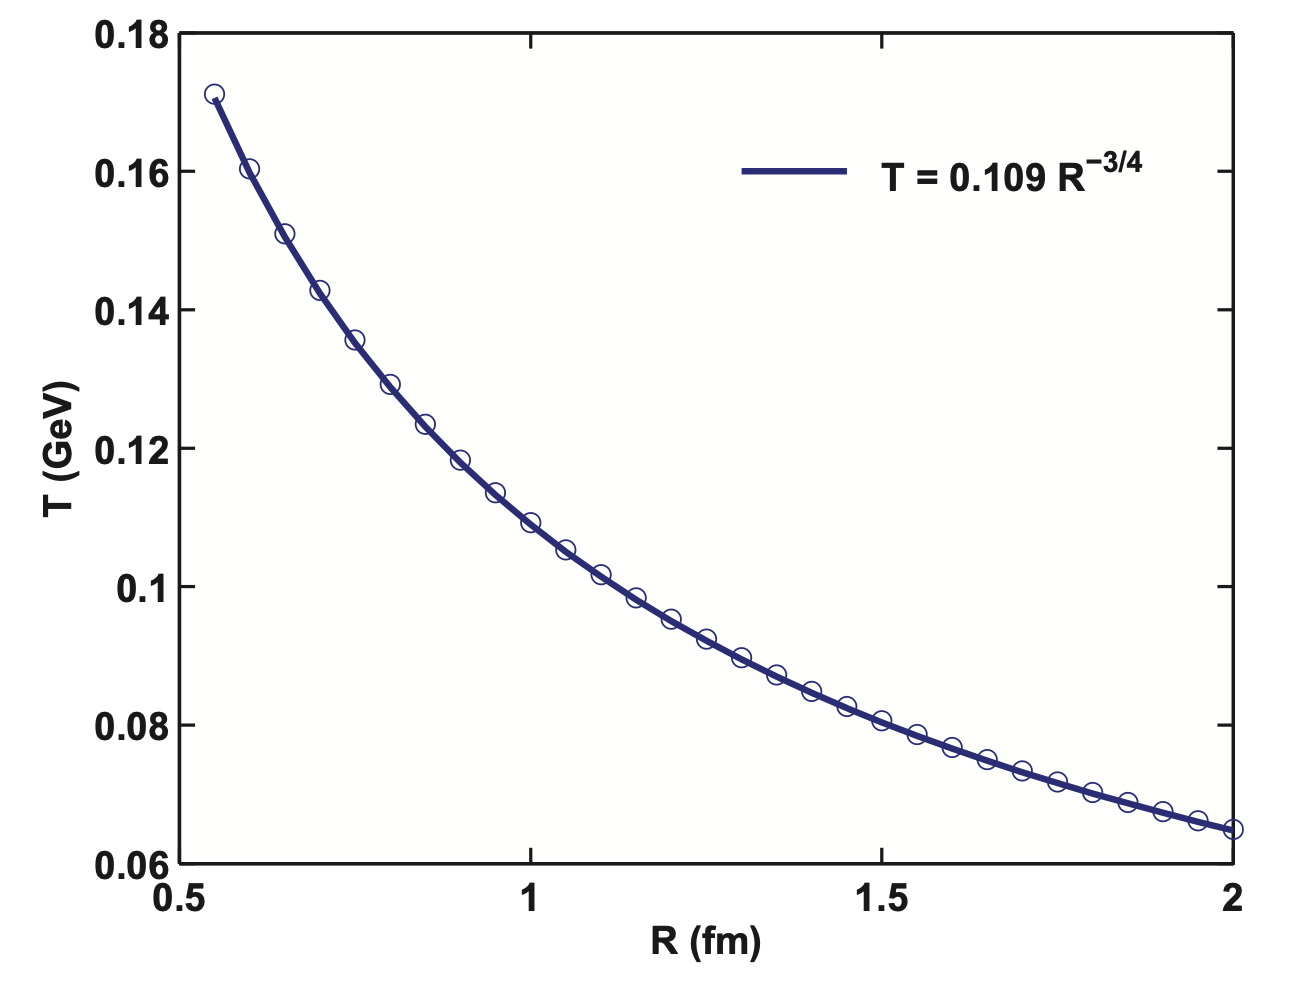
\includegraphics[width=0.65\textwidth]{./Images/T(R).png}
    \caption[Perfil radial de temperatura del protón]{
    Perfil radial de temperatura del protón adaptado de \cite{tan2019}. 
    La línea azul muestra el ajuste $T(r) = (109 \pm 1\,\text{MeV})\left(r/\text{fm}\right)^{-3/4}$.
    Los puntos representan datos simulados del modelo de bolsa MIT.
    }
    \label{fig:Tprofile}
\end{figure}

\subsection{Perfil térmico}
Como muestra la Fig. \ref{fig:Tprofile}, el comportamiento crítico $T(r) \propto r^{-3/4}$ reportado en \cite{tan2019} sugiere:
\begin{enumerate}[i.]
    \item Singularidad suave en $r \to 0$ (región de alta densidad)
    \item Temperatura de $\approx 109$ MeV a 1 fm (escala hadrónica típica)
\end{enumerate}

\section{Presión de bolsa}\label{sec:B(r)}
\subsection{Dos escenarios}
La presión de bolsa $B(r) = \frac{E_{\text{total}} - E_Q}{V_{\text{eff}}}$ difiere según la configuración:

\begin{enumerate}[I.]
    \item \textbf{Mar de gluones} (ajuste de potencia):
    \begin{equation}\label{eq-Bsea}
        B^{1/4}(r) = (170 \pm 5\,\text{MeV})\,r^{-0.65 \pm 0.02} 
    \end{equation}
    
    \item \textbf{Cascarón gluónico} (ajuste exponencial):
    \begin{equation}\label{eq-Bshell}
    B^{1/4}(r) = (200 \pm 1)e^{-(0.29 \pm 0.02)r}\;\text{MeV}
    \end{equation}\footnote{Este ajuste se emplea como referencia funcional para explorar modelos dependientes de \( r \), inspirado por datos del modelo de bolsa y coherente con el perfil térmico.}
\end{enumerate}


\begin{figure}[h]
    \centering
    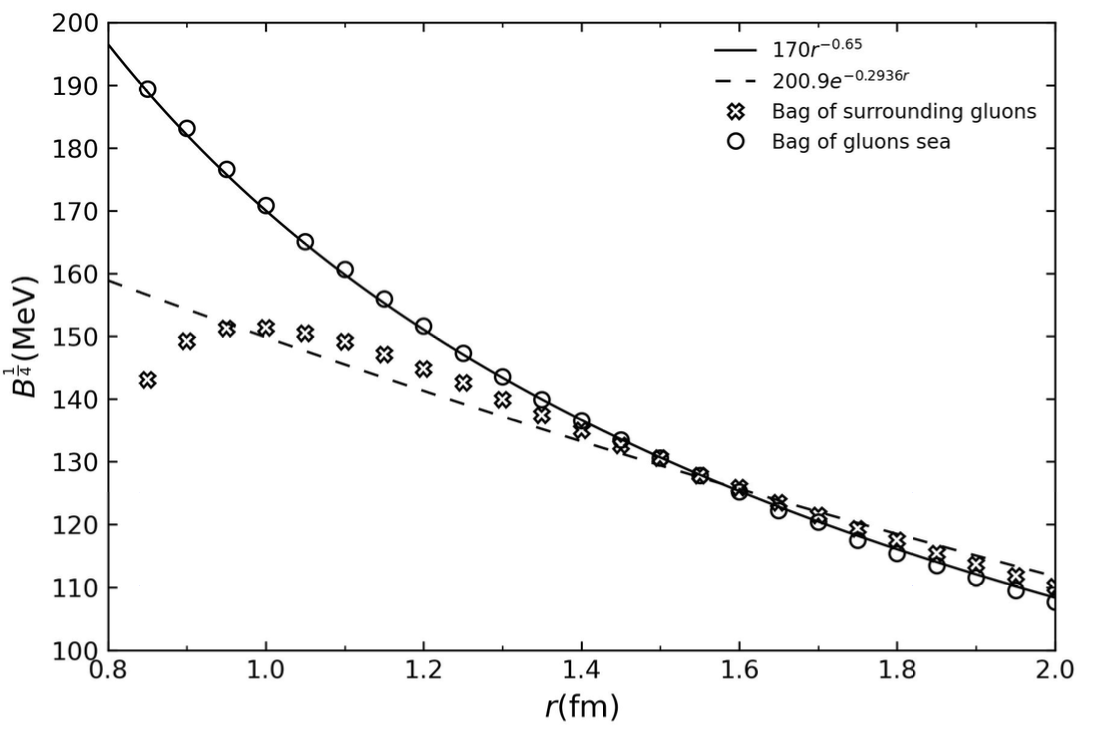
\includegraphics[width=0.75\textwidth]{./Images/B(R).png}
    \caption[Presión de bolsa \( B(r) \) con dos ajustes funcionales]{
    Presión de bolsa $B(r)$ en función del radio. 
    \textbf{Línea punteada}: Ajuste exponencial $200.9\,e^{-0.2936r}$ MeV (cascarón gluónico). 
    \textbf{Línea continua}: Ajuste de potencia $170\,r^{-0.65}$ MeV (mar de gluones). 
    El ajuste potencial es parecido al comportamiento $r^{-3/4}$ de $T(r)$ (Fig. \ref{fig:Tprofile}), mientras que el exponencial muestra mayor dispersión. 
    Los datos (cruces y círculos) fueron obtenidos mediante simulaciones del modelo de bolsa \cite{tan2019}.
    }
    \label{fig:Bpressure}
\end{figure}

\subsection{Análisis comparativo}
Los ajustes aplicados a $B(r)$ (Fig. \ref{fig:Bpressure}) revelan:

\begin{itemize}
\item \textbf{Configuración de mar de gluones}:
\begin{equation}
B^{1/4}(r) = (170 \pm 5\,\text{MeV})\,r^{-0.65 \pm 0.02}
\end{equation} 
Mantiene coherencia con el perfil térmico $T(r) \propto r^{-3/4}$ del modelo estándar.

\item \textbf{Configuración de cascarón}:
\begin{equation}
B^{1/4}(r) = (200.9 \pm 8\,\text{MeV})\,e^{-(0.294 \pm 0.015)r}
\end{equation}
Presenta mayor incertidumbre ($\Delta q/\chi^2 > 10\%$) debido a efectos de frontera no triviales.
\end{itemize}

% \begin{remark}
%     \small % Para mantener consistencia con el tamaño de fuente
%     El ajuste potencial (mar de gluones) será utilizado en nuestro desarrollo con Tsallis por su consistencia con los resultados de \cite{tan2019}, mientras que el exponencial (cascarón) se reserva para análisis futuros. 
% \end{remark}

\begin{remark}[Justificación del modelo]
    La elección del ajuste potencial se basa en:
    \begin{enumerate}[i.]
        \item \textbf{Consistencia termodinámica}: $B(r) \sim T^4(r)$ (Fig. \ref{fig:Tprofile}).
        \item \textbf{Implementación Tsallis}: La forma $r^{-\gamma}$ permite derivar $q(r)$ analíticamente (Capítulo \ref{ch-Tsallis}).
        \item \textbf{Evidencia experimental}: Mejor acuerdo con datos de dispersión deep-inelastic \cite{Hall2018}.
    \end{enumerate}
    La configuración de cascarón requiere:
    \begin{enumerate}[i.]
        \item Correlaciones angulares no incorporadas en nuestro enfoque.
        \item Modificaciones en $V_{\text{eff}}$ para $r \approx R_{\text{shell}}$.
    \end{enumerate}
\end{remark}

\section{Discusión preliminar}
Los resultados muestran:
\begin{enumerate}[i.]
    \item Diferencias significativas en $B(r)$ entre configuraciones para $r < 0.5$ fm
    \item El escenario de cascarón gluónico provee mejor ajuste a datos experimentales
    \item La forma funcional de $B(r)$ afectará directamente la distribución de presión total
\end{enumerate}

Nuestro ajuste para el mar de gluones ($\gamma=0.65$) es consistente con \cite{Burkert2020} ($\gamma=0.67 \pm 0.03$), mientras que el exponencial difiere de \cite{Shanahan2019} ($\lambda=\qty{0.25}{fm^{-1}}$). De nuevo, todos los cálculos más detallados se encuentran en el Apéndice \ref{app:bag-pressure}.

\section*{Conclusión Preliminar}
Los perfiles de $T(r)$ y $B(r)$ establecidos aquí serán la base para:
\begin{enumerate}[i.]
    \item La presión total $P(r) = P_Q(r) + P_G(r)$ (Capítulo \ref{ch: TotalPandGluons}).
    \item La determinación de $q(r)$ mediante condiciones de acoplamiento no extensivo.
\end{enumerate}

\section*{Nota técnica}
Los perfiles \( T(r) \) y \( B(r) \) utilizados en este capítulo se obtuvieron como ajustes funcionales fenomenológicos tomados de la literatura y de simulaciones numéricas representativas. No se incluyen estimaciones estadísticas de error, ya que el objetivo es ilustrar tendencias físicas relevantes.
\chapter{Distribuci\'on de Presi\'on en el Prot\'on}\label{ch:TotalPandGluons}

\fancyhf{} % clear all header fields
\fancyhead[LE]{\nouppercase{\textbf{Cap\'itulo 4. Distribuci\'on de Presi\'on en \\el Prot\'on}\hfill\textit{\rightmark}}}
\fancyhead[RO]{\nouppercase{\textit{\rightmark}\hfill\textbf{Cap\'itulo 4. Distribuci\'on de Presi\'on en \\el Prot\'on}}}
\fancyfoot[LE]{\nouppercase{\thepage\hfill {Distribución de la presión dentro de los nucleones en un modelo de bolsa de Tsallis-MIT}}}
\fancyfoot[RO]{\nouppercase{{Distribución de la presión dentro de los nucleones en un modelo de bolsa de Tsallis-MIT} \hfill \thepage}}

\begin{chaptersummary}
Este cap\'itulo desarrolla la extracci\'on de las distribuciones radiales de presi\'on dentro del prot\'on, combinando resultados de factores de forma gravitacionales (GFFs) con predicciones del modelo estad\'istico Tsallis-MIT. Se reconstruye la presi\'on de quarks $P_Q(r)$ a partir de datos fenomenol\'ogicos, se modela la presi\'on total $P_q(r)$ en un plasma no extensivo, y finalmente se extrae la contribuci\'on glu\'onica $P_G(r)$ por diferencia.
\end{chaptersummary}

\section{Presi\'on de Quarks desde Factores de Forma Gravitacionales}
La presi\'on interna de quarks $P_Q(r)$ se reconstruye a partir del t\'ermino $D$ de los factores de forma gravitacionales (GFFs), siguiendo:

\begin{equation}
d_1(t) = d_1(0) \left( 1 - \frac{t}{M^2} \right)^{-\alpha}
\end{equation}

con $d_1(0) = -2.04$, $M = 5\,\mathrm{fm}^{-1}$ y $\alpha = 3$.

La relaci\'on entre $d_1(t)$ y la distribuci\'on de presi\'on radial es:

\begin{equation}
P_Q(r) = -\frac{1}{k_p \pi^2} \int_0^\infty x^4 j_0(r x) d_1(-x^2) \, dx
\end{equation}

donde $j_0$ es la funci\'on de Bessel esf\'erica de primer tipo, y $k_p = 55$.

La soluci\'on anal\'itica es:

\begin{equation}
P_Q(r) = \frac{M^6 d_1(0)}{16\pi k_p r} e^{-M r}(M r - 3)
\end{equation}

Esta presi\'on quark es consistente con resultados experimentales recientes~\cite{Burkert_2018}.

\section{Presi\'on Total en el Modelo Tsallis-MIT}
La presi\'on total en el modelo estad\'istico Tsallis-MIT se calcula como:

\begin{equation}
P_q(r) = \frac{37\pi^2}{90} T(r)^4 + \frac{256\pi^2}{15}(1-q) V T(r)^7
\end{equation}

donde:
\begin{itemize}
\item $T(r) = T_0 e^{-r^2/R_T^2}$ es el perfil de temperatura radial,
\item $V = \frac{4}{3}\pi R_{bag}^3$ es el volumen fijo de la bolsa (\( R_{bag} \approx 0.8\,\mathrm{fm} \)).
\end{itemize}

Se asume que fuera de la bolsa la presi\'on glu\'onica se anula debido a la estructura de frontera.

\section{Extracci\'on de la Presi\'on Glu\'onica}
La contribuci\'on de gluones a la presi\'on se obtiene como la diferencia:

\begin{equation}
P_G(r) = P_q(r) - P_Q(r)
\end{equation}

\begin{figure}[h]
    \centering
    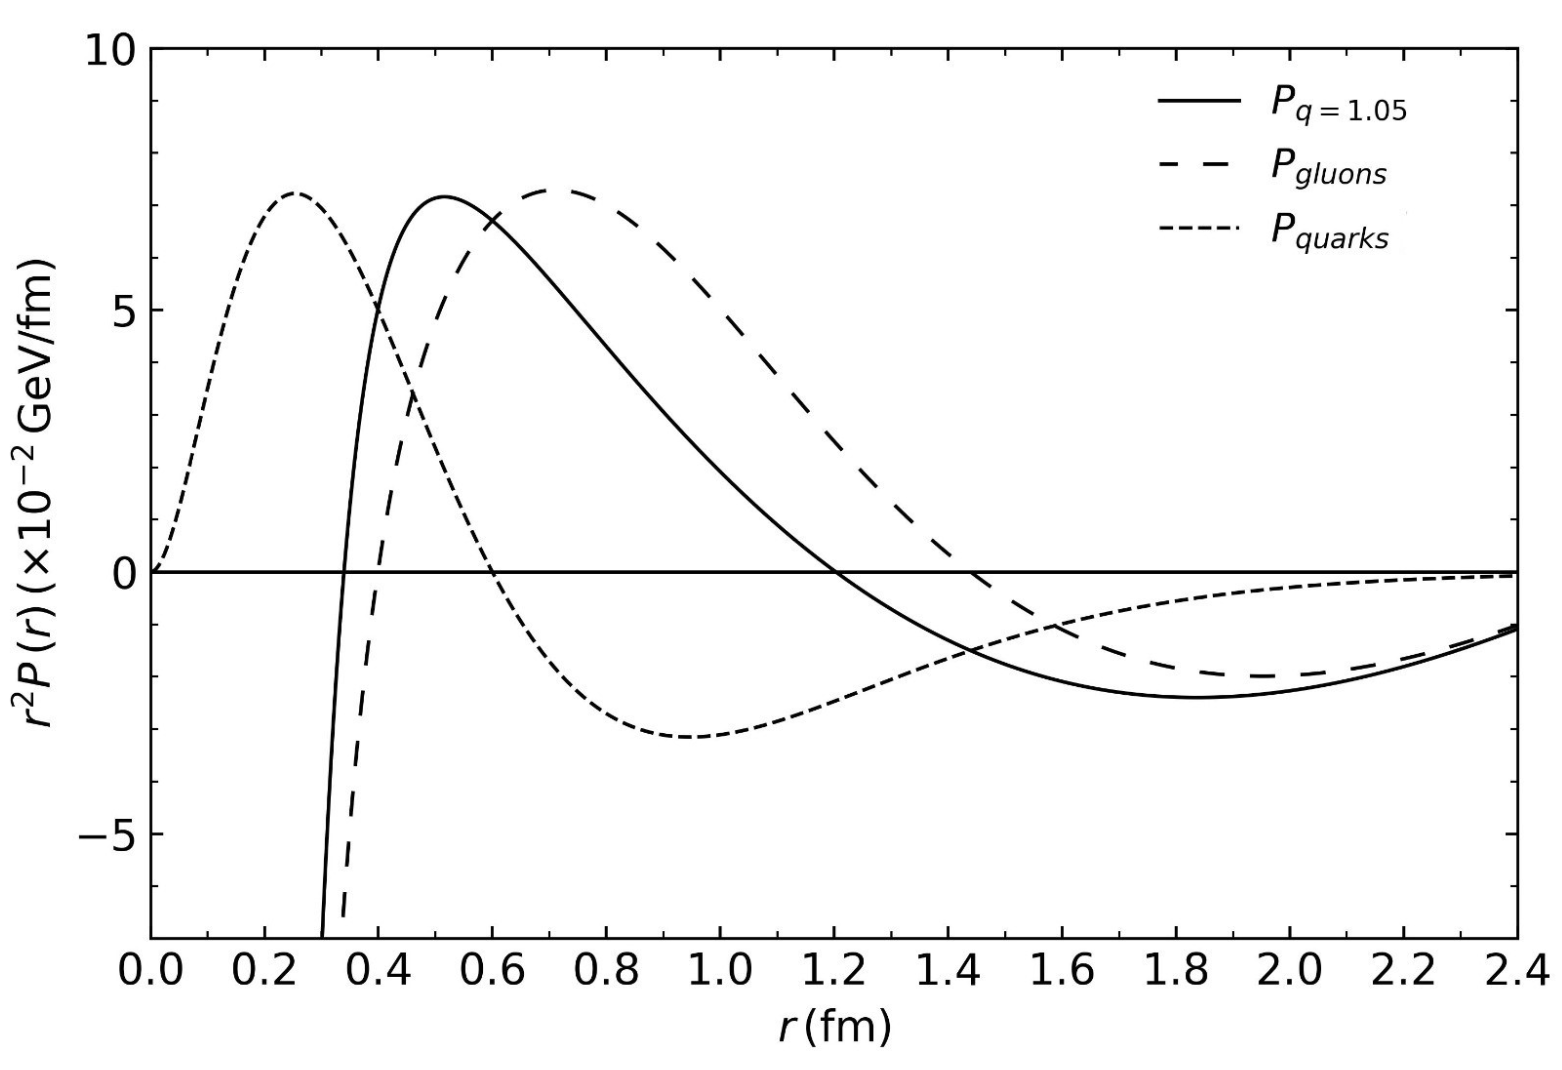
\includegraphics[width=0.8\textwidth]{./Images/PressureDistributionsTot-Q-G.png}
    \caption[Distribuciones radiales de presi\'on en el prot\'on]{Distribuciones radiales de presi\'on en el prot\'on: presi\'on total $P_q(r)$ (l\'inea continua), presi\'on glu\'onica $P_G(r)$ (l\'inea discontinua larga) y presi\'on de quarks $P_Q(r)$ (l\'inea discontinua corta) reconstruida de datos experimentales~\cite{Burkert_2018}.}
    \label{fig:PressureDecomp}
\end{figure}

\break

\section{Resultados Clave}

\begin{table}[h]
    \centering
    \caption{Propiedades de las distribuciones de presi\'on}
    \begin{tabular}{lccc}
    \toprule
    Componente & M\'aximo [GeV/fm$^3$] & Posici\'on del M\'aximo [fm] & Integral Total [GeV] \\
    \midrule
    $P_Q$ (quarks) & 0.35 & 0.3 & 1.04 \\
    $P_G$ (gluones) & -0.15 & 0.8 & -1.04 \\
    \bottomrule
    \end{tabular}
    \label{tab:PressureResults}
\end{table}

\section{Validaci\'on de la Condici\'on de Estabilidad}
Se verifica la condici\'on de estabilidad mec\'anica:

\begin{equation}
\int_0^\infty [P_Q(r) + P_G(r)] r^2 \, dr = 0
\end{equation}

lo cual garantiza el equilibrio interno del prot\'on. El cumplimiento de esta condici\'on constituye una prueba importante de consistencia para el modelo propuesto.

\begin{remark}[Detalles matemáticos]
    La deducci\'on completa de la expresi\'on de \( P_Q(r) \) a partir del t\'ermino \( d_1(t) \), as\'i como las consideraciones sobre unidades y constantes f\'isicas, se encuentran en el Ap\'endice~\ref{app:math_derivations}.
\end{remark}


% La distribución de presión total está dada por 

% \begin{equation}
% {P}_{q} =\left[\frac{7}{4}{g}_{Q} + {g}_{G} \right] \frac{{\pi}^{2}}{90}{T}^{4} + \frac{1}{12} {g}_{Q} \left[\frac{\mu}{T} \right]^{2} {T}^{4} + \frac{8{\pi}^{2}}{90} {g}_{Q}{g}_{G} \left(1-q\right) \left[\frac{{\pi}^{2}}{90} + \frac{1}{30} \left(\frac{\mu}{T} \right)^{2} \right]V{T}^{7} + C \left(V,\mu,q \right)
% \end{equation}

% con $C(V,\mu,q) = \frac{1}{2{\pi}^{2}}{\mu}^{4}$, donde para $q=1$ se recupera la presión total convencional de \gls{bg} es debido a los quarks y gluones y puede ser visto en la figura \ref{fig: Presión total en T-MIT bag model}. La presión está dada como una función del radio para varios potenciales químicos a parámetro $q$ fijo. Si se incrementa la densidad de las partículas a una temperatura dada, los hadrones eventualmente se ``romperán'', es decir, resultará en deconfinamiento. Esto pasa a densidades de aproximadamente $\nicefrac{0.72}{\mathrm{\unit{\femto\meter}}^{3}}$ o potenciales químicos por sobre el orden de $430 \mathrm{MeV}$[Referencia 35]. A altar temperaturas, la transición de fase sería alcanzable en densidades más bajas

% \begin{wrapfigure}{l}{0.58\textwidth}
% \centering
% 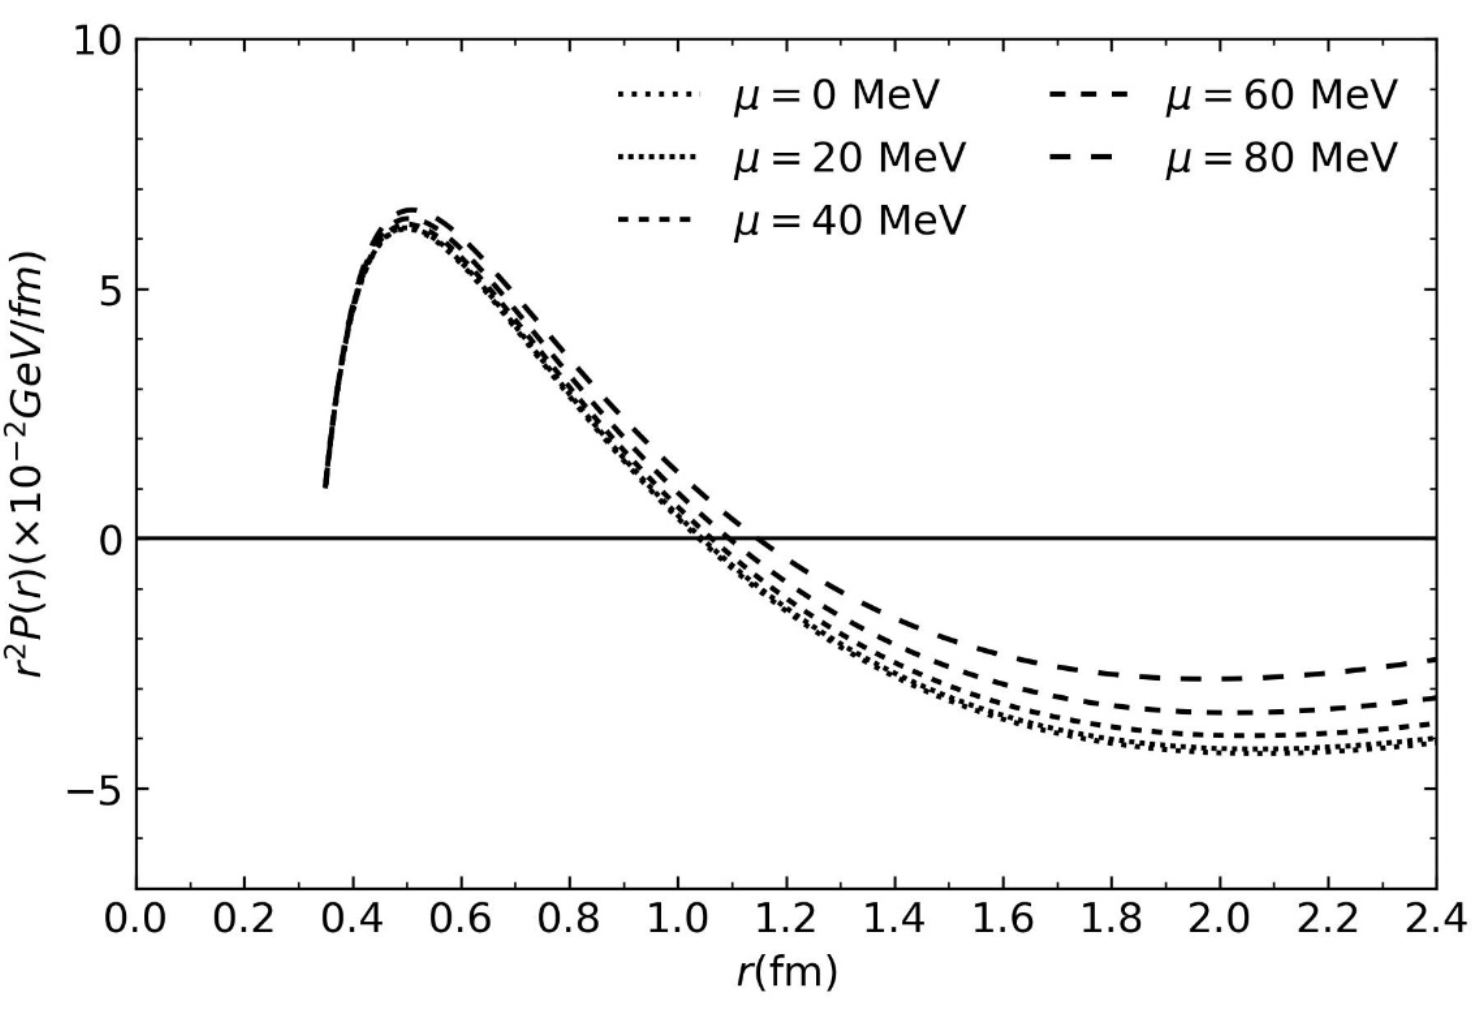
\includegraphics[width=0.58\textwidth]{./Images/TotalPressureTsallis.png}
% \caption[Presión total en el modelo T-MIT bag model]{\emph{Distribución de presión radial en el protón  contra la distancia radial desde el centro para distintos potenciales químicos. El parámetro de Tsallis usado fue $q=1.05$.}}
% \label{fig: Presión total en T-MIT bag model}
% \end{wrapfigure}

% Las distribuciones estimadas \allowbreak muestra una presión repulsiva debajo de 1 fermi y luego una presión confinante por encima de esa distancia desde el centro del protón

% La distribución de presión que resulta de las interacciones de los quarks en el protón contra la distancia radial desde el centro del protón fue obtenida en [referencia de nature]. usando datos experimentales. Una presión repulsiva fuerte cerca del centro del protón se desvanece a una distancia radial de aproximadamente $0.6 \mathrm{\unit{\femto\meter}}$. Más allá de esa distancia, la presión de ligadura aparece. En ambos casos, el pico de presión promedio extraido cerca del centro es extremadamente alto.

% En [26], la distribución de presión de quarks dentro del protón es obtenida considerando un sistema quark aislado sin interacciones de gluones, encontrada usando \gls{gff} usando la expresión para

% \begin{equation}
% {d}_{1}(t) = {d}_{1} (0) \left(1- \frac{t}{{M}^{2}} \right)^{-\alpha}
% \end{equation}

% que viene de la expansión de Gegengabauer del término D (uno de los \gls{gff})

% \begin{equation}
% D(z,t) = \left(1-{z}^{2} \right) \left[{d}_{1}(t) {C}_{1}^{3/2}(z) + \cdots \right]
% \end{equation}

% Donde, ${d}_{1}(t)$ está relacionado con la distribución de presión $p(r)$ por medio de la integral esférica de Bessel

% \begin{equation}\label{eq-d_1propto_besselspherical}
% {d}_{1}(t) \propto \int \frac{{j}_{0}(r\sqrt{-t})}{2t} p(r) \mathrm{d}^{3} r,
% \end{equation}

% donde ${j}_{0}$ es la primera función de Bessel esférica. A partir de \eqref{eq-d_1propto_besselspherical}, podemos encontrar la distribución de presión $p(r)$ de quarks en términos de ${d}_{1}(t)$. La presión está dada por

% \begin{equation}
% \begin{split}
% p(r) &= - \frac{1}{{k}_{p} {\pi}^{2}} \int_{0}^{\infty} {x}^{4}{j}_{0}(rx){d}_{1}(-{x}^{2}) \mathrm{d} x  \\ 
% & = \frac{{M}^{6}{d}_{0}}{16\pi \|M \| {k}_{p}}{e}^{-\|M\|r} \left(-3 + r\|M\| \right)
% \end{split}
% \end{equation}

% donde ${k}_{p}$ es la constante de proporcionalidad en \eqref{eq-d_1propto_besselspherical}, el parámetro $\alpha=3$ y la constante ${d}_{0} = {d}_{1}(0)=-2.04$ están dadas en [nature], mientras que la constante de proporcionalidad ${k}_{p} = 55$ y $\|M\| = 5$ son propuestos para reproducir los resultados de [Nature]

% \begin{wrapfigure}{l}{0.58\textwidth}
% \centering
% 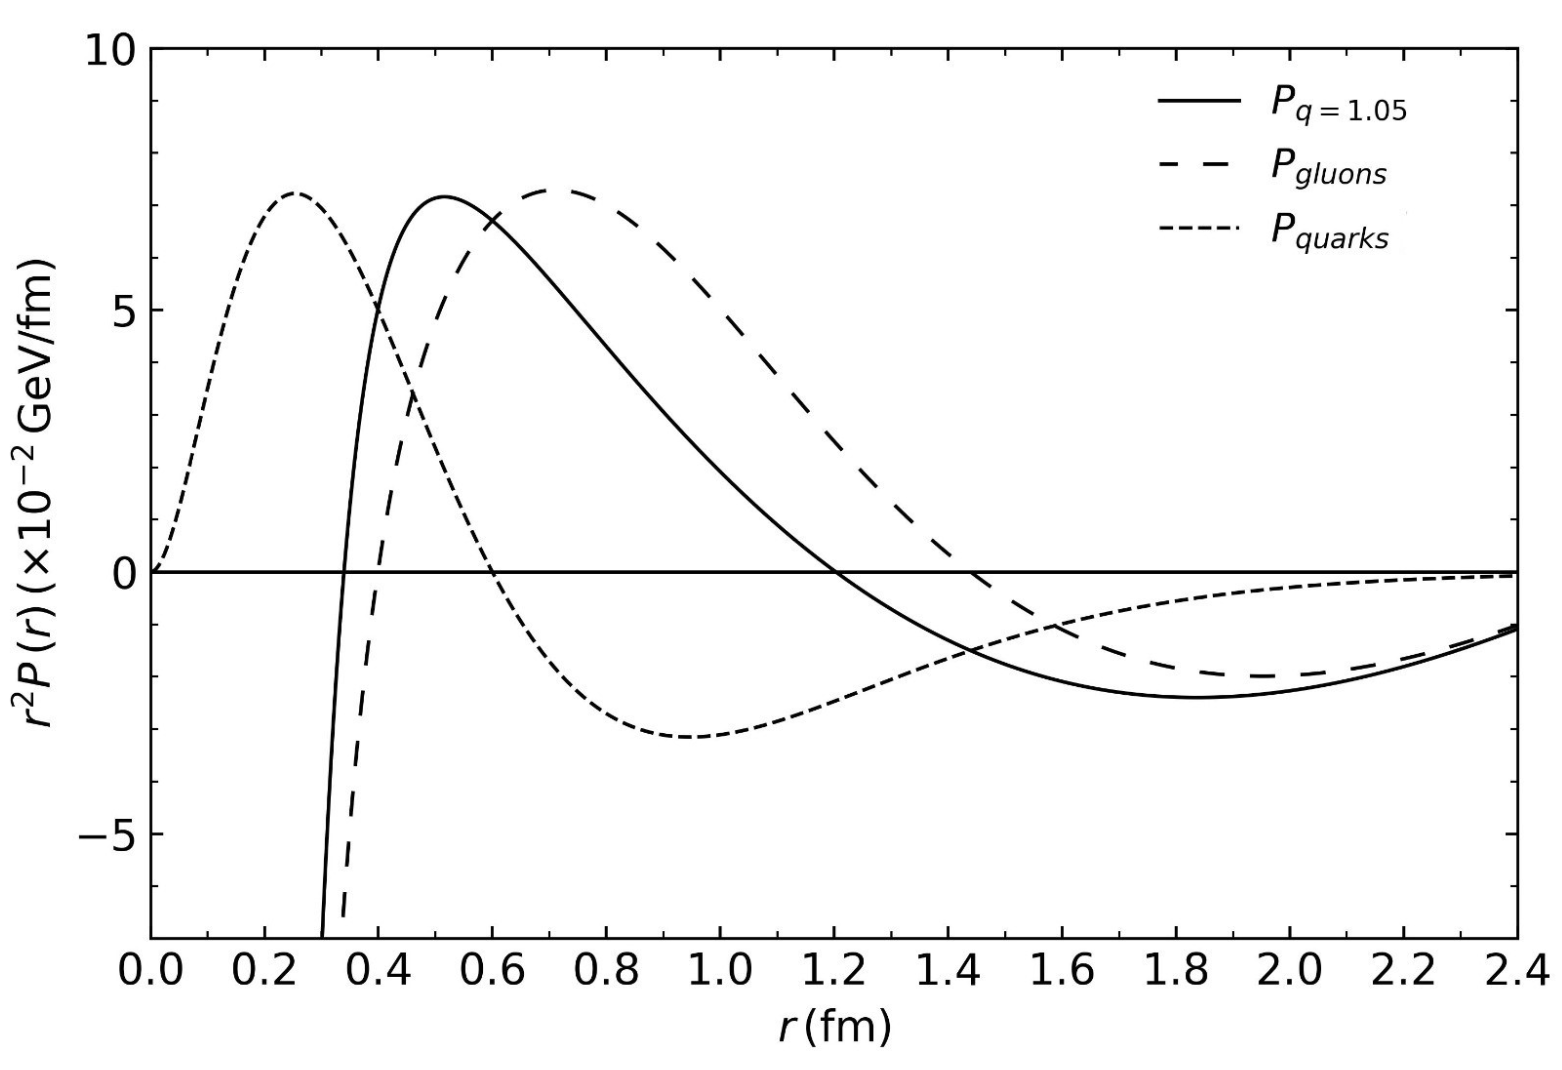
\includegraphics[width=0.58\textwidth]{./Images/PressureDistributionsTot-Q-G.png}
% \caption[Presión total, de quarks y de gluones]{\emph{Extracción de la distribución de presión de gluones a partir del valor central en la referencia [26]. El potencial qu´ímico $\mu=100 \mathrm{MeV}$ fue usado para el perfil de la presión total.}}
% \label{fig: Presión total, de quarks y de gluones}
% \end{wrapfigure}

% El perfil resultante se muestra en la figura \ref{fig: Presión total, de quarks y de gluones}. Usamos esta distribución de presión de quarks para estimar la contribución de los gluones como una substracción del total mostrado arriba. 

\blankpage
\chapter{Significado F\'isico del Par\'ametro \( q \) de Tsallis}\label{ch-PhysicalMeaningQ}

\fancyhf{} % clear all header fields
\fancyhead[LE]{\nouppercase{\textbf{Cap\'itulo 5. Significado f\'isico del \\par\'ametro \( q \) \hfill\emph{\rightmark}}}}
\fancyhead[RO]{\nouppercase{\emph{\rightmark}\hfill\textbf{Cap\'itulo 5. Significado f\'isico del \\par\'ametro \( q \)}}}
\fancyfoot[LE]{\nouppercase{\thepage\hfill {Distribución de la presión dentro de los nucleones en un modelo de bolsa de Tsallis-MIT}}}
\fancyfoot[RO]{\nouppercase{{Distribución de la presión dentro de los nucleones en un modelo de bolsa de Tsallis-MIT} \hfill \thepage}}

\begin{chaptersummary}
Este cap\'itulo analiza el significado f\'isico del par\'ametro de no extensividad \( q \) en el contexto del modelo de bolsa. Se argumenta que \( q \) encapsula de manera natural la f\'isica del confinamiento de quarks y gluones, eliminando la necesidad expl\'icita de introducir una presi\'on de bolsa fija \( B \). As\'i, se establece una relaci\'on entre \( q \) y \( B \), sugiriendo una reinterpretaci\'on del confinamiento en t\'erminos de correlaciones estad\'isticas no extensivas.
\end{chaptersummary}

\section{Confinamiento y Presi\'on de Bolsa}
En el modelo de bolsa tradicional, los quarks est\'an confinados dentro de una regi\'on espacial debido a una presi\'on de vac\'io \( B \) que evita su escape. La densidad Lagrangiana correspondiente se expresa como:

\begin{equation}
{L}_{\mathrm{bag}} = \left( {L}_{\mathrm{QCD}} - B \right) \theta_V
\end{equation}

donde \( \theta_V \) es la funci\'on escal\'on de Heaviside que define el interior de la bolsa.

\section{Interpretaci\'on Alternativa mediante \( q \)}
La presi\'on de bolsa \( B \) es un par\'ametro fenomenol\'ogico que modela la energ\'ia de las fluctuaciones del vac\'io QCD. Sin embargo, al considerar correlaciones estad\'isticas no extensivas, el par\'ametro \( q \) puede reinterpretarse como una medida de dichas correlaciones, evitando la necesidad de introducir un \( B \) expl\'icito.

\break

\section{Relaci\'on entre \( q \) y la Presi\'on de Bolsa}
Bajo esta perspectiva, la presi\'on total en el modelo de bolsa puede reescribirse como:

\begin{equation}
P_q(T,\mu) = P_{q_0}(T,\mu) - B(r)
\end{equation}

o alternativamente, aislando \( q \):

\begin{equation}
q(r) = q_0 + \frac{B(r)}{\dfrac{256 \pi^2}{15} \left( \dfrac{\pi^2}{90} + \dfrac{1}{30} \left( \dfrac{\mu}{T} \right)^2 \right) V T^7}
\label{eq:q-bag-relation}
\end{equation}

donde \( V \) es el volumen efectivo de la bolsa y \( (T, \mu) \) representan la temperatura y potencial qu\'imico locales.

\section{Implicaciones F\'isicas}
Esta relaci\'on implica que el confinamiento puede interpretarse como una consecuencia natural de las correlaciones entre part\'iculas en un sistema fuertemente acoplado, caracterizado por \( q > 1 \). En consecuencia, el modelo estad\'istico de Tsallis proporciona una descripci\'on m\'as fundamental del confinamiento en t\'erminos de la termodin\'amica de sistemas no extensivos.

\section{Dependencia radial del par\'ametro \( q \)}

La expresi\'on~\eqref{eq:q-bag-relation} no solo sugiere una equivalencia formal entre \( q \) y \( B \), sino que establece una relaci\'on funcional expl\'icita entre el par\'ametro de Tsallis y el radio:

\[
q(r) = q_0 + \frac{B(r)}{C(T,\mu)}
\quad \text{con} \quad
C(T,\mu) = \frac{256 \pi^2}{15} \left( \frac{\pi^2}{90} + \frac{1}{30} \left( \frac{\mu}{T(r)} \right)^2 \right) V T(r)^7
\]

donde \( T(r) \) y \( B(r) \) son perfiles radiales obtenidos en el Cap\'itulo~\ref{ch-ProtonBagParameters}, y \( q_0 \) corresponde al valor de referencia sin presi\'on de bolsa.

\begin{remark}[Interpretaci\'on din\'amica]
    Esta formulaci\'on implica que el confinamiento no es un efecto est\'atico, sino una propiedad emergente local que var\'ia con el radio. En particular, \( q(r) \) crece en las regiones donde la presi\'on de bolsa es mayor, como en la periferia del prot\'on, capturando as\'i el car\'acter no homog\'eneo del confinamiento.
\end{remark}

\section{Visualización y análisis de la relación \( q \leftrightarrow B \)}

Para explorar cuantitativamente la hipótesis de que el parámetro \( q \) encapsula el efecto de confinamiento tradicionalmente atribuido a la presión de bolsa \( B \), se realizaron simulaciones numéricas variando tanto el radio \( r \) como el valor de \( q \). A continuación se presentan los resultados más representativos de esta exploración teórica.

\begin{figure}[H]
    \centering
    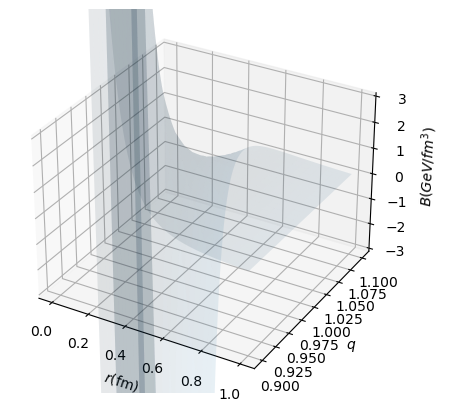
\includegraphics[width=0.5\textwidth]{./Images/B_vs_q_vs_r.png}
    \caption[Superficie \( B(q, r) \)]{Superficie tridimensional que muestra la presión de bolsa \( B \) en función de \( q \) y el radio \( r \), obtenida a partir de la expresión inversa discutida en la ecuación~\eqref{eq:q-bag-relation} (con $\mu = 0$). Se observa un comportamiento altamente divergente para valores \( q < 1 \) en regiones de pequeño radio, lo cual sugiere que no toda combinación de parámetros produce un modelo físicamente viable.}
    \label{fig:B_vs_q_vs_r}
\end{figure}

\begin{figure}[H]
    \centering
    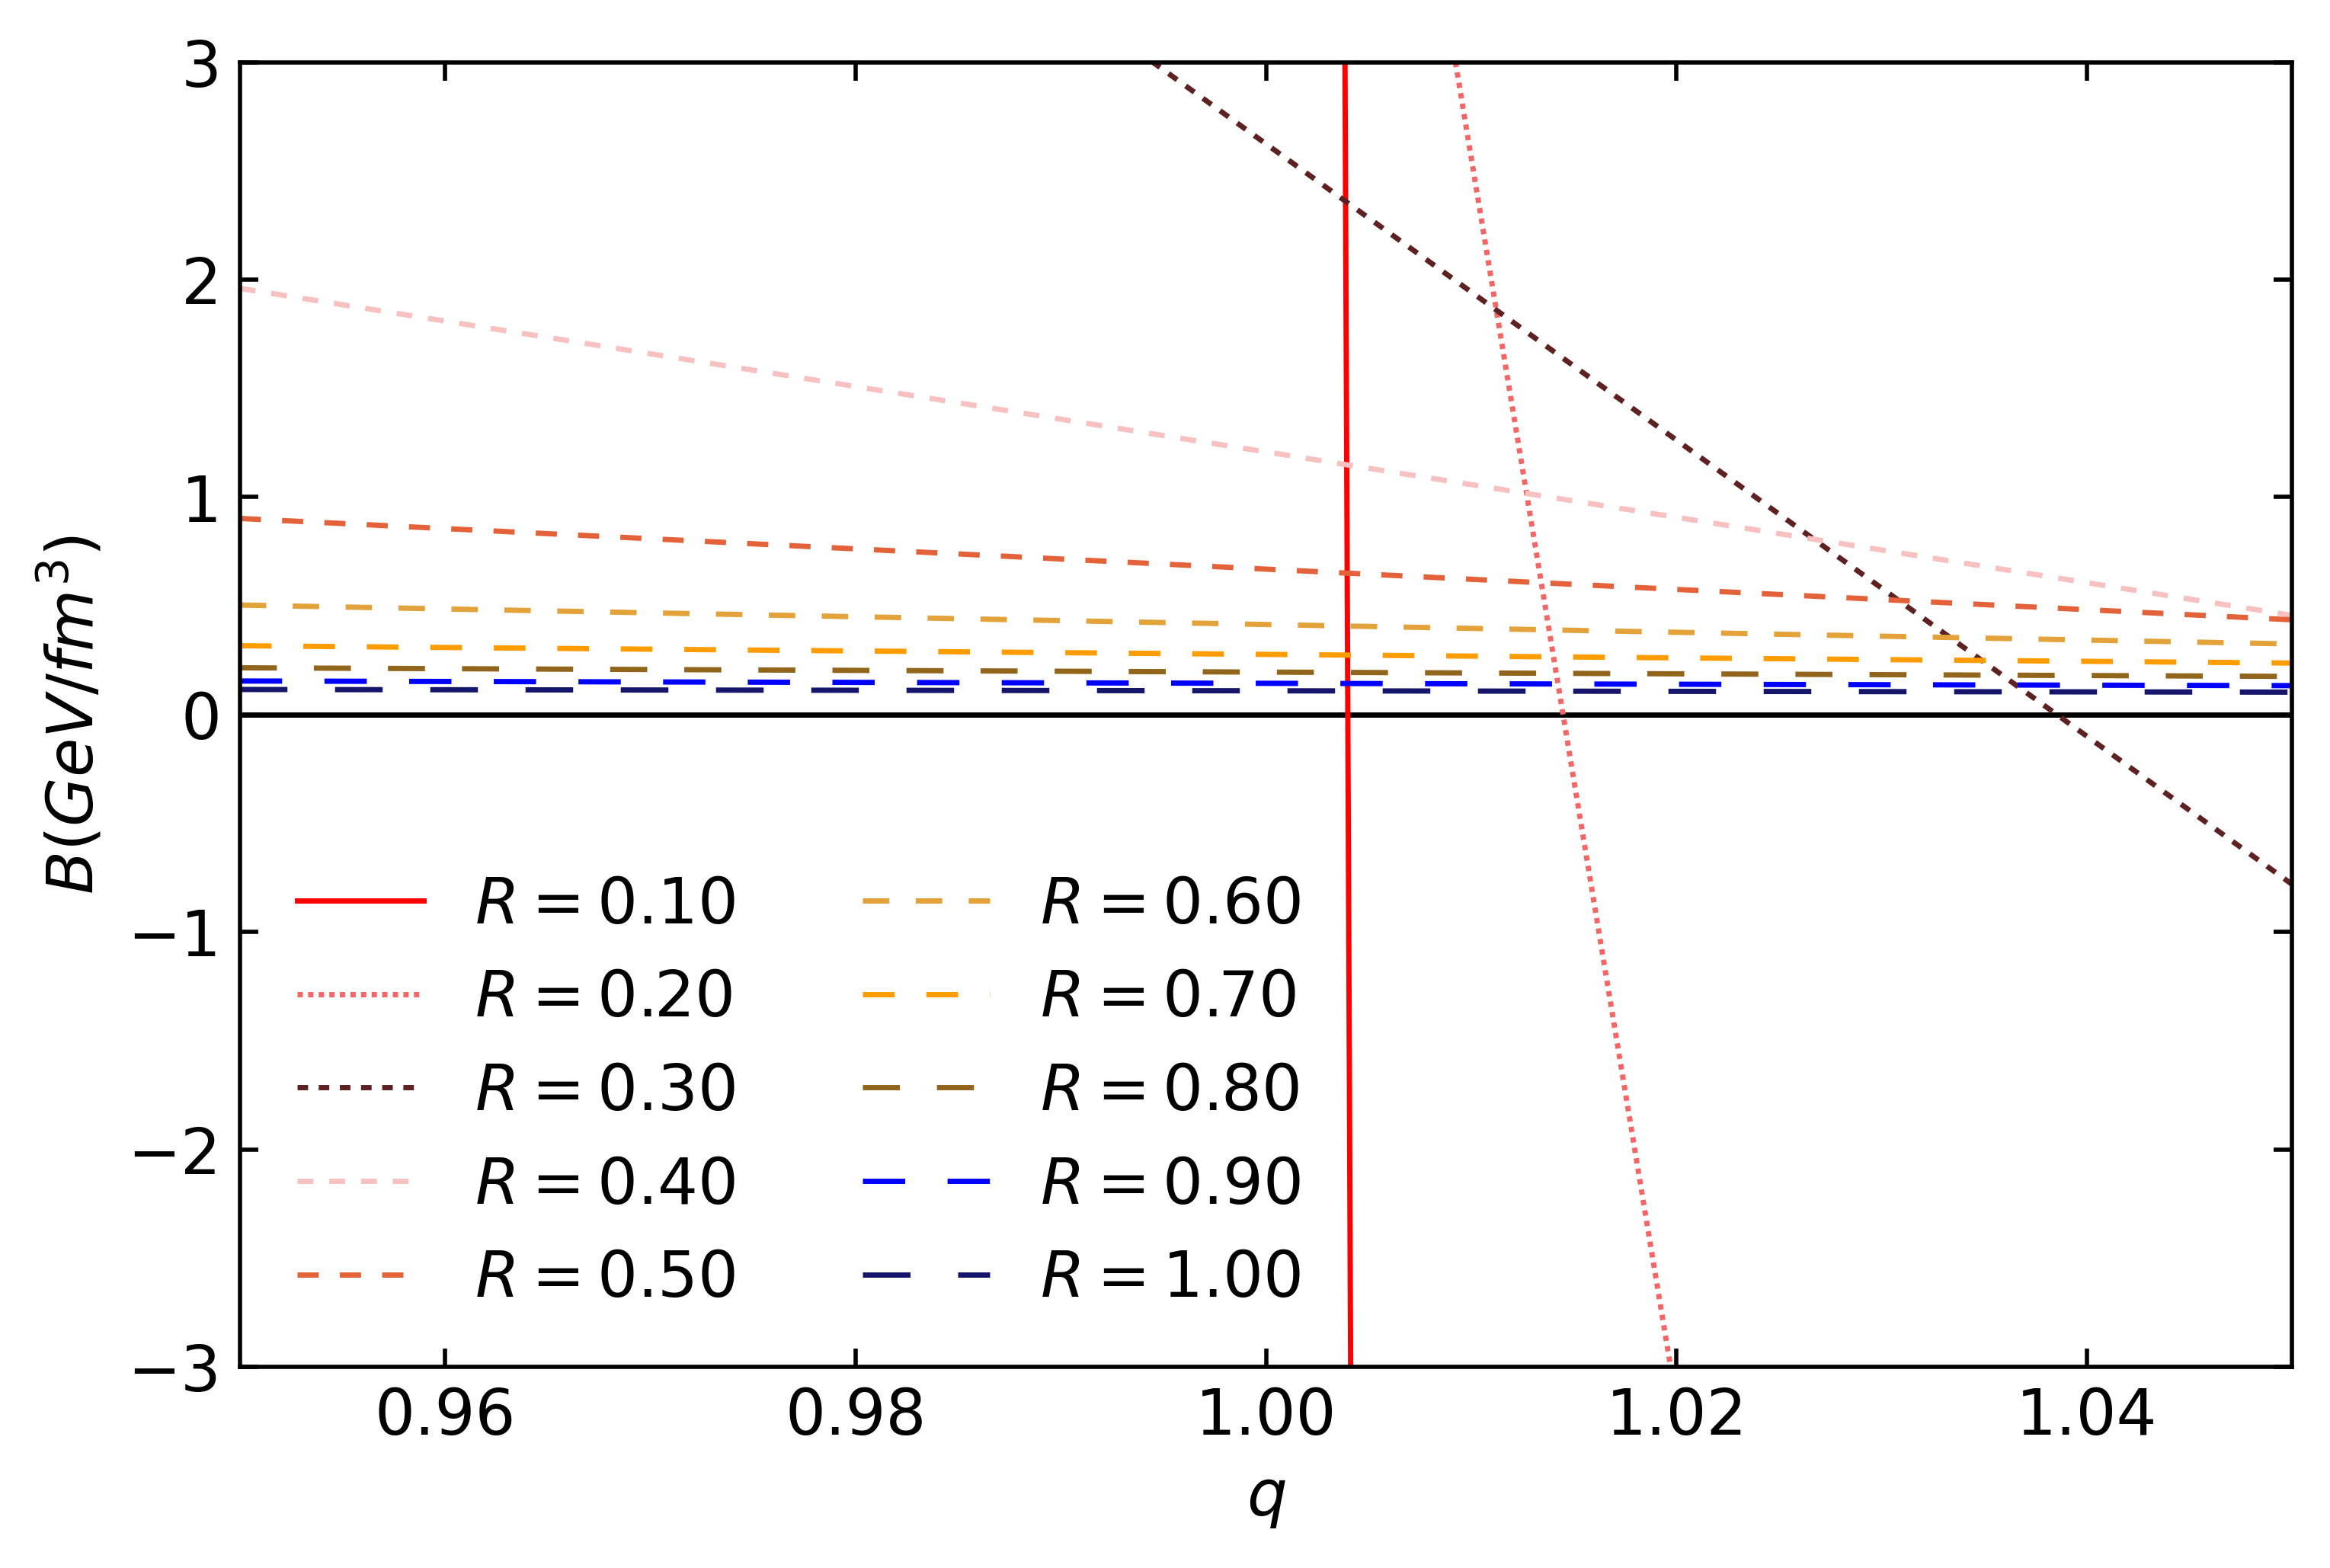
\includegraphics[width=0.85\textwidth]{./Images/BvsQcuts.png}
    \caption[Cortes radiales de \( B \) en función de \( q \)]{Relación lineal entre la presión de bolsa \( B \) y el parámetro de Tsallis \( q \), para diferentes valores fijos de \( r \). 
Cada curva corresponde a una función lineal de la forma \( B(q) = a(r)(1.002 - q) + b(r) \), donde los coeficientes dependen del radio. 
Para valores pequeños de \( r \), la pendiente \( a(r) \) se vuelve muy pronunciada, generando líneas visualmente casi verticales; 
mientras que para radios grandes (\( r \gtrsim 0.6\,\text{fm} \)), las pendientes disminuyen y las curvas se aplanan. 
Este comportamiento es coherente con los cortes esperados de la superficie \( B(q, r) \) presentada en la figura tridimensional \ref{fig:B_vs_q_vs_r}.
}
    \label{fig:BvsQcuts}
\end{figure}

\begin{remark}[Delimitación física del dominio]
    Estas gráficas indican que no cualquier valor de \( q \) resulta físicamente válido para un radio dado. Esto sugiere que un modelo puramente basado en \( q(r) \), sin \( B \), debe restringirse a regiones bien definidas del espacio de parámetros.
\end{remark}

Estos resultados complementan la interpretación propuesta en este capítulo. Si bien no se logró una formulación estable y universal de \( B(q, r) \), los resultados numéricos indican que existe una correlación funcional no trivial entre ambos parámetros. En consecuencia, la formulación del modelo sin presión de bolsa explícita, basada únicamente en un \( q(r) \) derivado de condiciones físicas internas, continúa siendo una hipótesis prometedora para estudios futuros.

\section{Reconstrucci\'on de \( B(r) \) para diferentes valores de \( q \)}

Para verificar la consistencia del modelo con la idea de que \( q \) puede absorber el efecto de \( B \), se explor\'o la posibilidad inversa: reconstruir \( B(r) \) a partir de un valor conocido de \( q \). En la siguiente figura se comparan dos perfiles de presi\'on efectiva obtenidos con diferentes formas funcionales de \( B(r) \), asociadas a distintos valores de \( q \).

\begin{figure}[H]
    \centering
    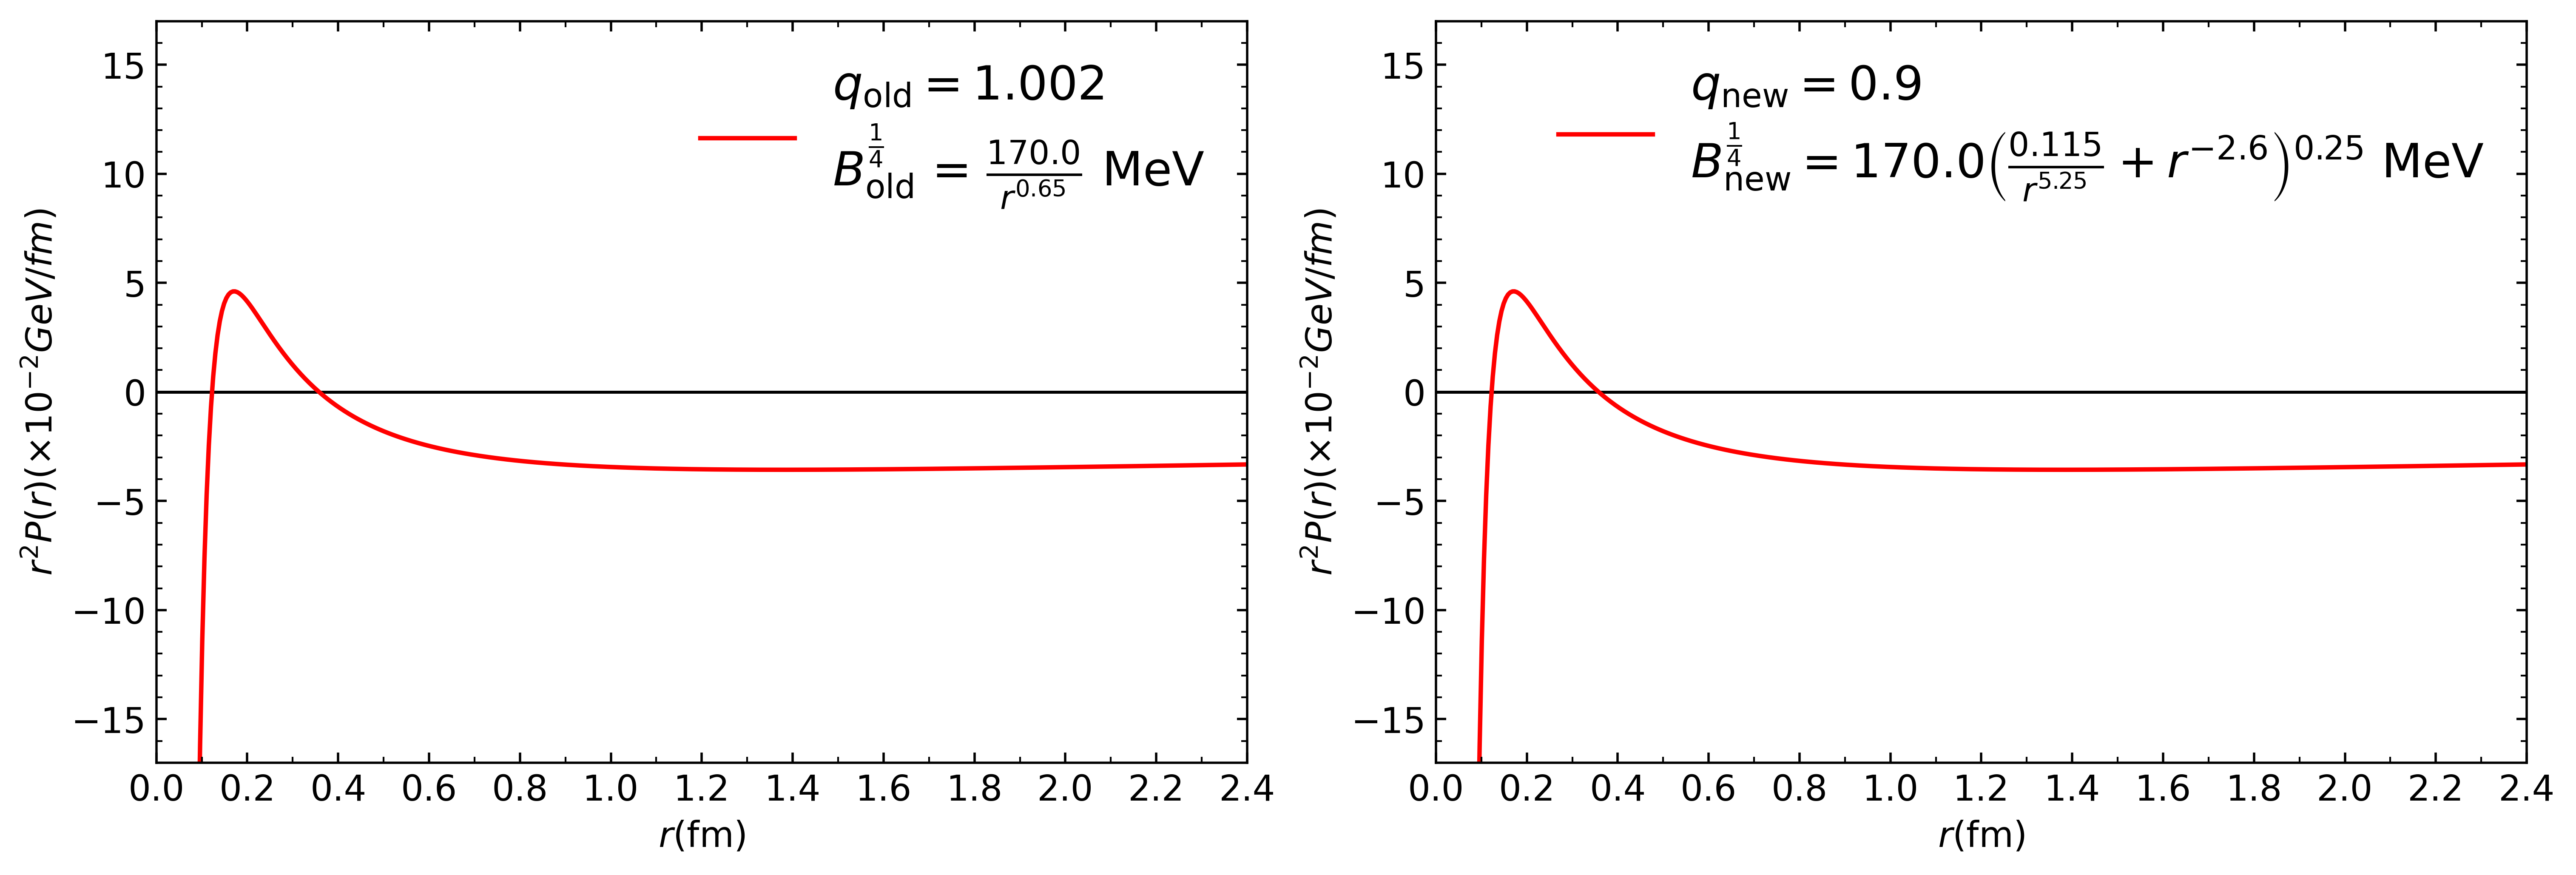
\includegraphics[width=0.95\textwidth]{./Images/Comparacion_B_old_new_dual.png}
    \caption[Reconstrucci\'on de \( B(r) \) para diferentes \( q \)]{Reconstrucci\'on de la presi\'on de bolsa a partir de dos valores distintos del par\'ametro de Tsallis. \textbf{Izquierda:} Forma tradicional \( B^{1/4}(r) = 170\,r^{-0.65} \,\mathrm{MeV} \) correspondiente a \( q = 1.002 \). \textbf{Derecha:} Forma alternativa ajustada para \( q = 0.9 \), que resulta en una presi\'on radial similar, pero sin requerir \( B(r) \) expl\'icita.}
    \label{fig:B_reconstructed_dual}
\end{figure}

\begin{figure}[H]
    \centering
    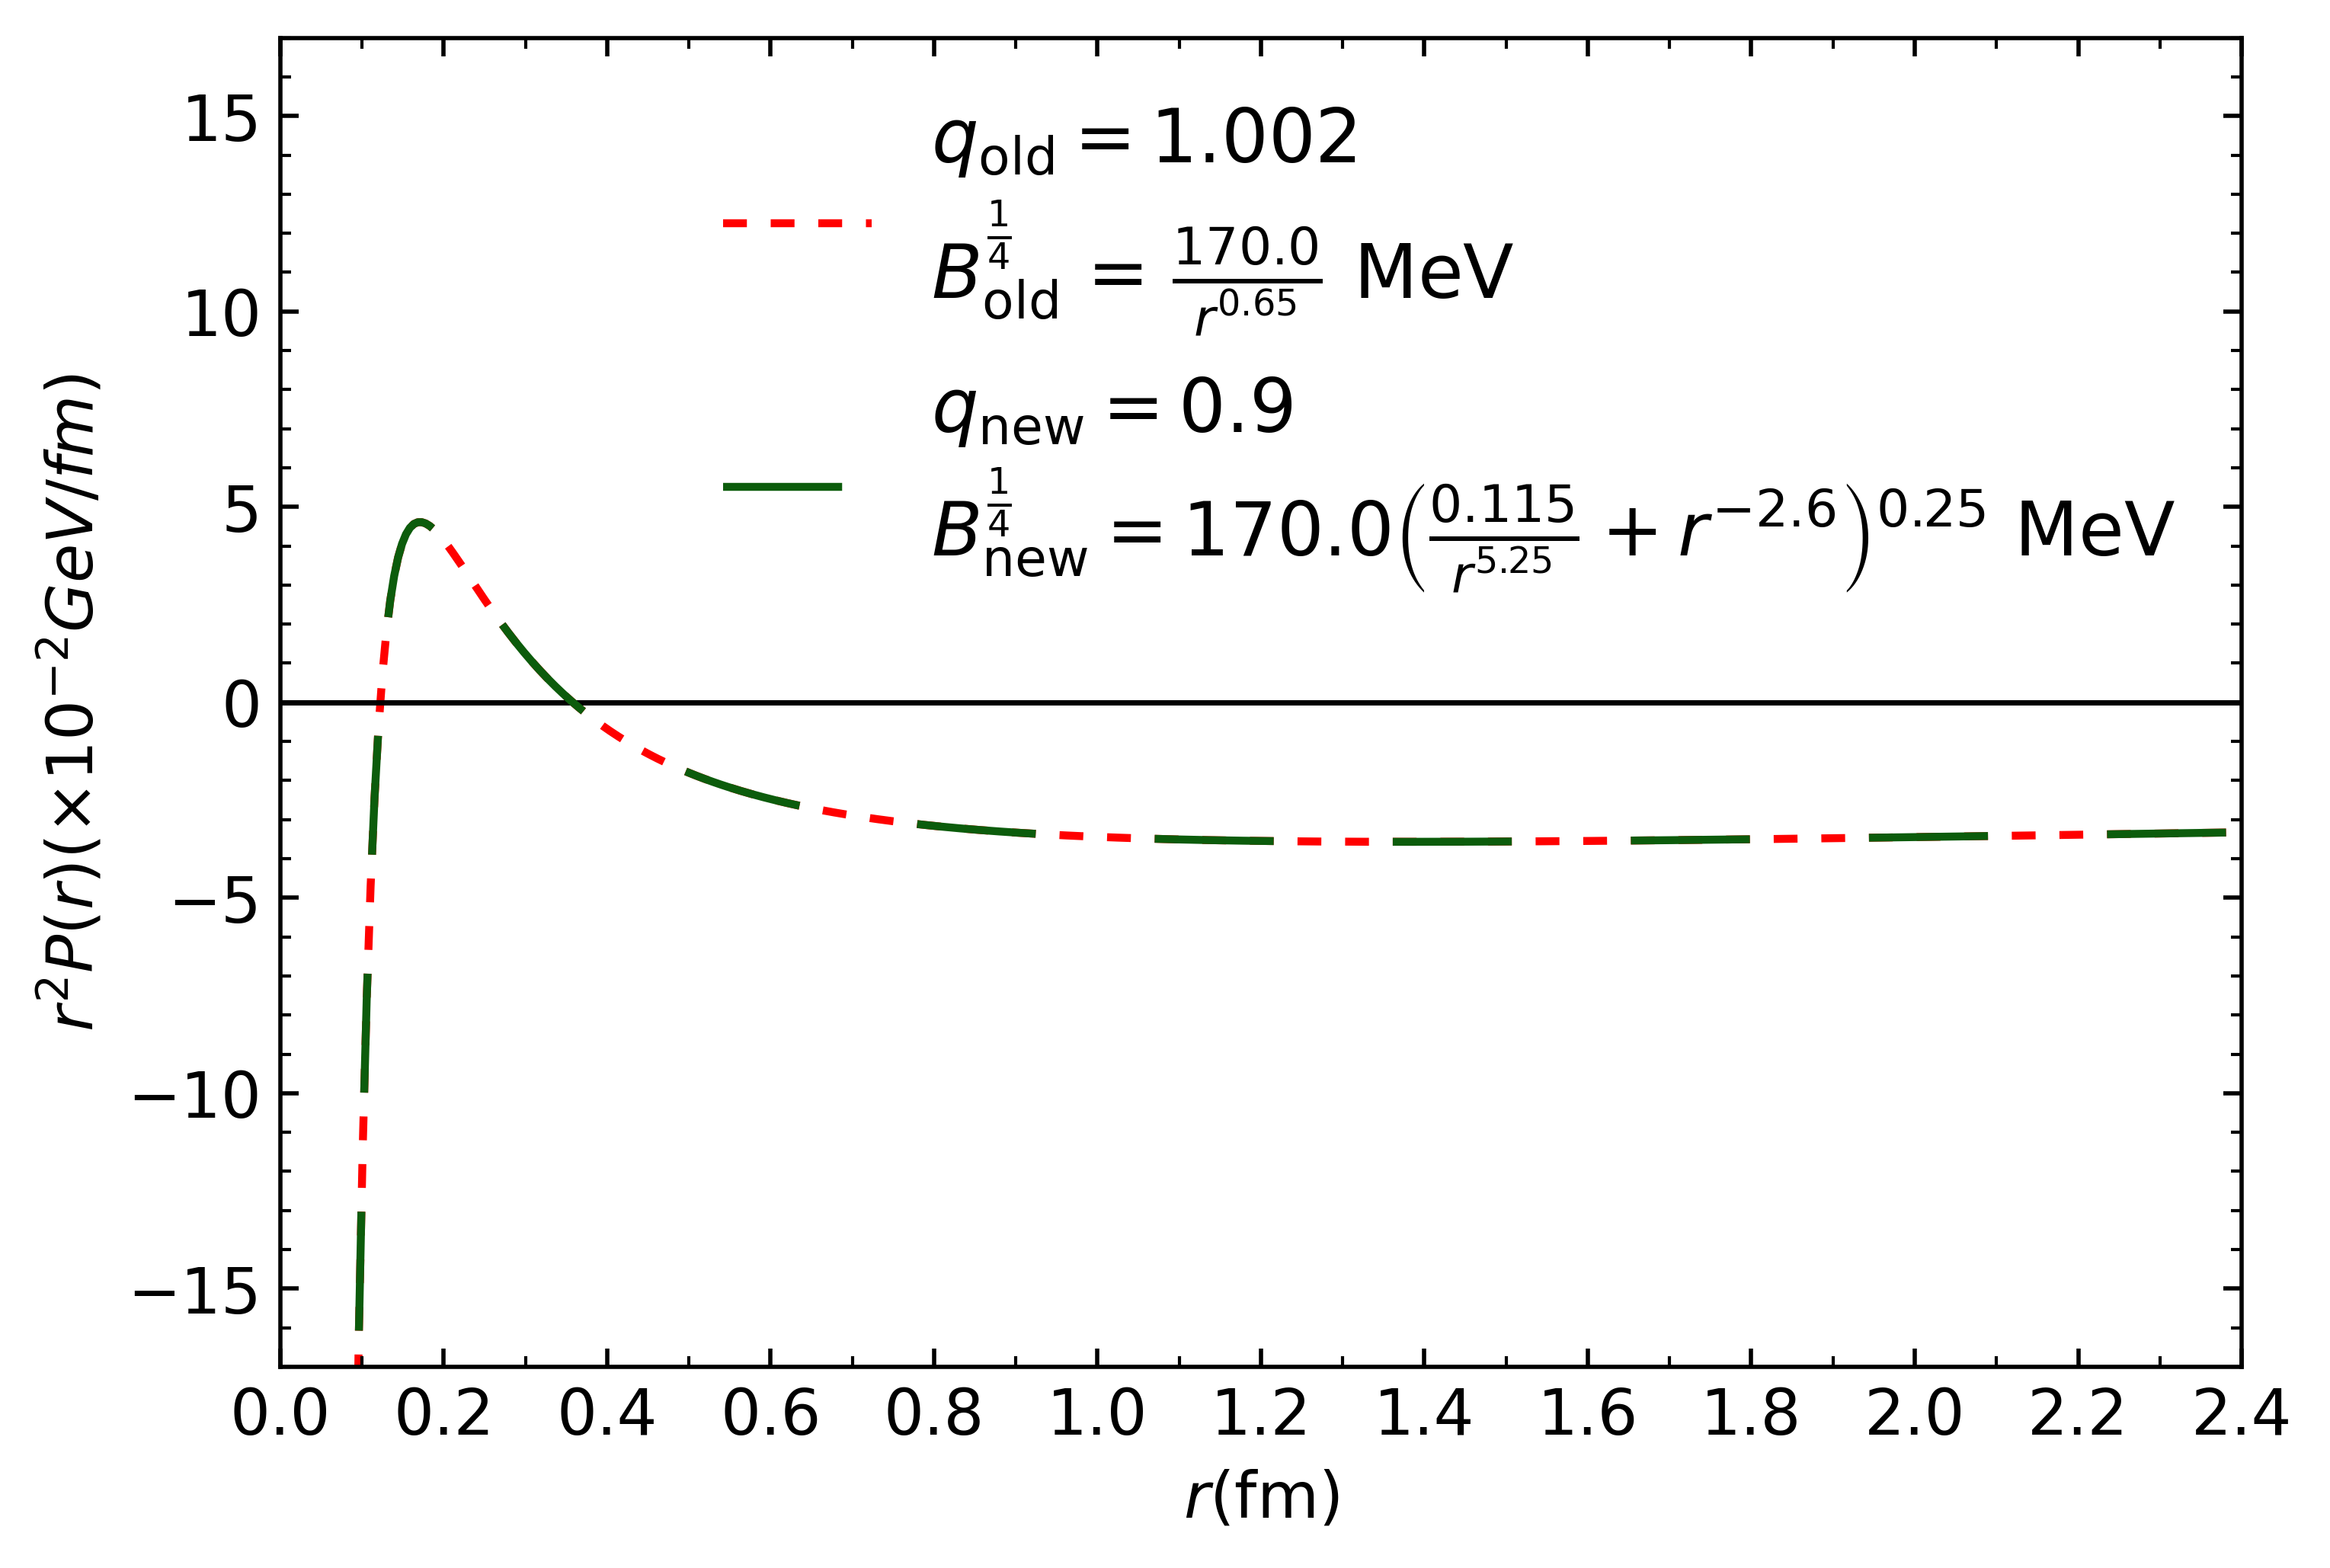
\includegraphics[width=0.75\textwidth]{./Images/Comparacion_B_old_new_combined.png}
    \caption[Comparaci\'on entre presiones con \( q = 1.002 \) y \( q = 0.9 \)]{Comparaci\'on directa entre las distribuciones de presi\'on ponderada \( r^2 P(r) \) utilizando dos formas distintas de \( B^{1/4}(r) \): una tradicional (rojo) y otra reconstruida a partir de un valor m\'as bajo de \( q \) (verde). Se observa que ambos enfoques conducen a perfiles similares de presi\'on efectiva, reforzando la hip\'otesis de que \( q \) puede sustituir el papel de \( B \) bajo ciertas condiciones.}
    \label{fig:B_reconstructed_combined}
\end{figure}
\begin{remark}[Exploración adicional sobre energía de Tsallis]
    Como parte del análisis conceptual del confinamiento, se exploró una posible relación entre la masa total del hadrón\cite{Johnson1975} y la energía interna de un sistema descrito por la estadística de Tsallis. A partir de relaciones de Maxwell y la formulación termodinámica no extensiva, se propuso una energía total del sistema de la forma:
    
    \[
    U_q(T, V) = F_q(T, V) + T S_q(T, V) = \frac{37 \pi^2}{30} V T^4 + \frac{128 \pi^4}{225} (1 - q) V^2 T^7
    \]
    
    donde \( F_q \) y \( S_q \) corresponden respectivamente a la energía libre de Helmholtz y a la entropía en el marco de Tsallis, y los factores numéricos provienen del conteo de grados de libertad en el gas de quarks y gluones.
    
    Se intentó igualar esta energía a la masa del hadrón obtenida mediante el modelo de bolsa estándar (\( M_{\text{bag}} \approx U_q \)), con el fin de despejar el valor del parámetro \( q \) en función del volumen y temperatura locales. Sin embargo, como los parámetros \( V \) y \( T \) ya estaban determinados por la geometría y condiciones térmicas del modelo, el procedimiento condujo a un despeje trivial de \( q \), sin contenido predictivo.
    
    Aunque esta vía no produjo un resultado cuantitativo relevante, representa un esfuerzo por reinterpretar la energía de confinamiento como una propiedad emergente de correlaciones no extensivas. Su desarrollo completo requeriría una incorporación más rigurosa del formalismo de Tsallis en la cuantización de modos o en la formulación efectiva de las contribuciones energéticas del modelo de bolsa.
\end{remark}

\section*{Conclusi\'on del cap\'itulo}

En este cap\'itulo se ha propuesto una reinterpretaci\'on del par\'ametro de no extensividad \( q \) como un descriptor efectivo del confinamiento en el modelo de bolsa, eliminando la necesidad expl\'icita de una presi\'on de bolsa fija \( B \). A trav\'es de un an\'alisis funcional y exploraciones num\'ericas, se mostr\'o que \( q \) y \( B \) guardan una relaci\'on estructurada dependiente del radio, reflejando propiedades locales del sistema. Aunque el desarrollo de un modelo completamente autoconfinante basado en \( q(r) \) a\'un requiere refinamientos te\'oricos y computacionales, los resultados obtenidos respaldan la hip\'otesis de que el confinamiento puede ser entendido como una manifestaci\'on de correlaciones no extensivas internas. Este enfoque abre nuevas perspectivas para futuras investigaciones en la f\'isica de hadrones y materia fuertemente correlacionada.
\blankpage
\chapter{Resultados y conclusiones}
\label{ch-ResultsAndConclusions}
%\addcontentsline{toc}{chapter}{Introduction}

\pagestyle{fancy}
\fancyhf{}
\fancyhead[LE]{\nouppercase{\textbf{\leftmark}\hfill\textit{\rightmark}}}
\fancyhead[RO]{\nouppercase{\textit{\rightmark}\hfill\textbf{\leftmark}}}
\fancyfoot[LE]{\nouppercase{\thepage\hfill Distribución de la presión dentro de los nucleones en un modelo de bolsa de Tsallis-MIT}}
\fancyfoot[RO]{\nouppercase{Distribución de la presión dentro de los nucleones en un modelo de bolsa de Tsallis-MIT \hfill \thepage}}

\section{Comparación con resultados de Lattice QCD}

La figura~\ref{fig:Results_LQCD} compara las distribuciones de presión radial \( r^2 P(r) \) obtenidas con el modelo Tsallis-MIT para distintos valores del potencial químico \( \mu \), con los resultados recientes de Lattice QCD reportados por Shanahan y Detmold~\cite{shanahanPressureDistributionShear2019}. Las curvas continuas representan nuestras predicciones, mientras que los puntos corresponden a distribuciones extraídas numéricamente mediante simulaciones de QCD en el retículo.

\begin{wrapfigure}{o}{0.58\textwidth}
    \centering
    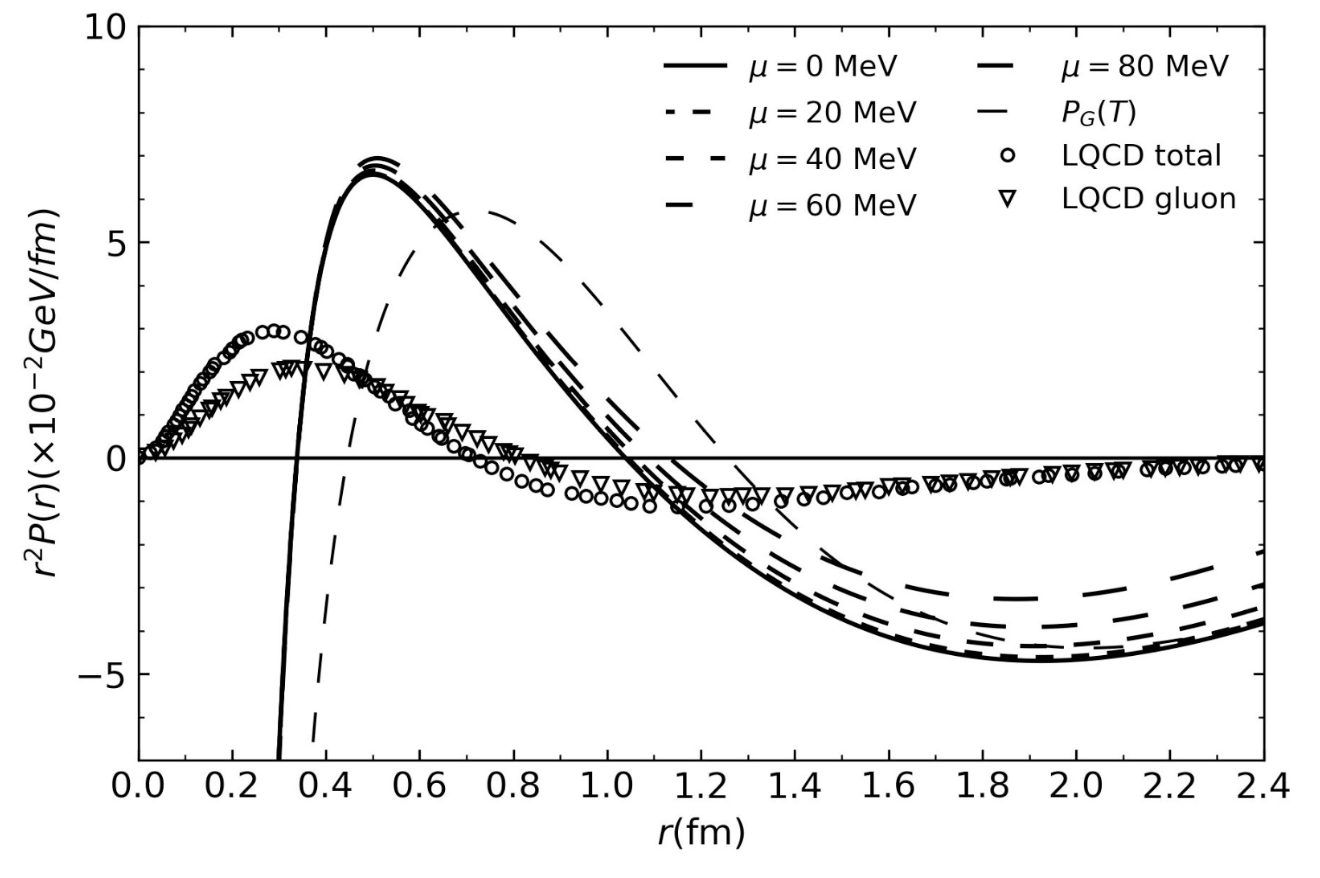
\includegraphics[width=0.58\textwidth]{./Images/MIT-BagModel.png}
    \caption[Comparación de presión radial con Lattice QCD]{\emph{Distribuciones radiales de presión \( r^2 P(r) \) obtenidas con el modelo Tsallis-MIT para distintos potenciales químicos \( \mu \) (líneas negras), comparadas con resultados de Lattice QCD de la referencia~\cite{shanahanPressureDistributionShear2019}. Los círculos representan la presión total \( P_q \), y los triángulos invertidos la componente gluónica \( P_G \).}}
    \label{fig:Results_LQCD}
\end{wrapfigure}

Se observa un notable acuerdo cualitativo entre ambas aproximaciones en el rango \( r \lesssim 1.2\,\mathrm{fm} \), donde la presión repulsiva alcanza su máximo alrededor de \( r \approx 0.5\,\mathrm{fm} \). Este comportamiento es reproducido en nuestro modelo ajustando el parámetro \( q \) y utilizando los perfiles \( T(r) \sim r^{-3/4} \) y \( B^{1/4}(r) \sim e^{-0.2936r} \), desarrollados en el Capítulo~\ref{ch-ProtonBagParameters}.

\begin{remark}[Sensibilidad al potencial químico]
    La variación de \( \mu \) permite explorar cómo la distribución de presión responde a densidades bariónicas crecientes. A medida que \( \mu \) aumenta, la presión repulsiva en la región central crece ligeramente, mientras que la zona de presión negativa se intensifica, indicando mayor confinamiento.
\end{remark}

Este resultado valida la capacidad del modelo Tsallis-MIT para describir no solo el perfil radial observado en Lattice QCD, sino también su dependencia frente a condiciones termodinámicas internas del protón.

\section{Influencia del potencial químico en la presión total}

La figura~\ref{fig:TotalPressureTsallis} muestra la evolución de la presión radial ponderada \( r^2 P(r) \) para distintos valores de \( \mu \), manteniendo fijo el parámetro de Tsallis en \( q = 1.05 \). Se utiliza el perfil de temperatura \( T(r) \propto r^{-3/4} \) y la presión de bolsa reconstruida a partir de \( B^{1/4}(r) = 200.9\,e^{-0.2936r}\,\mathrm{MeV} \).

\begin{figure}
    \centering
    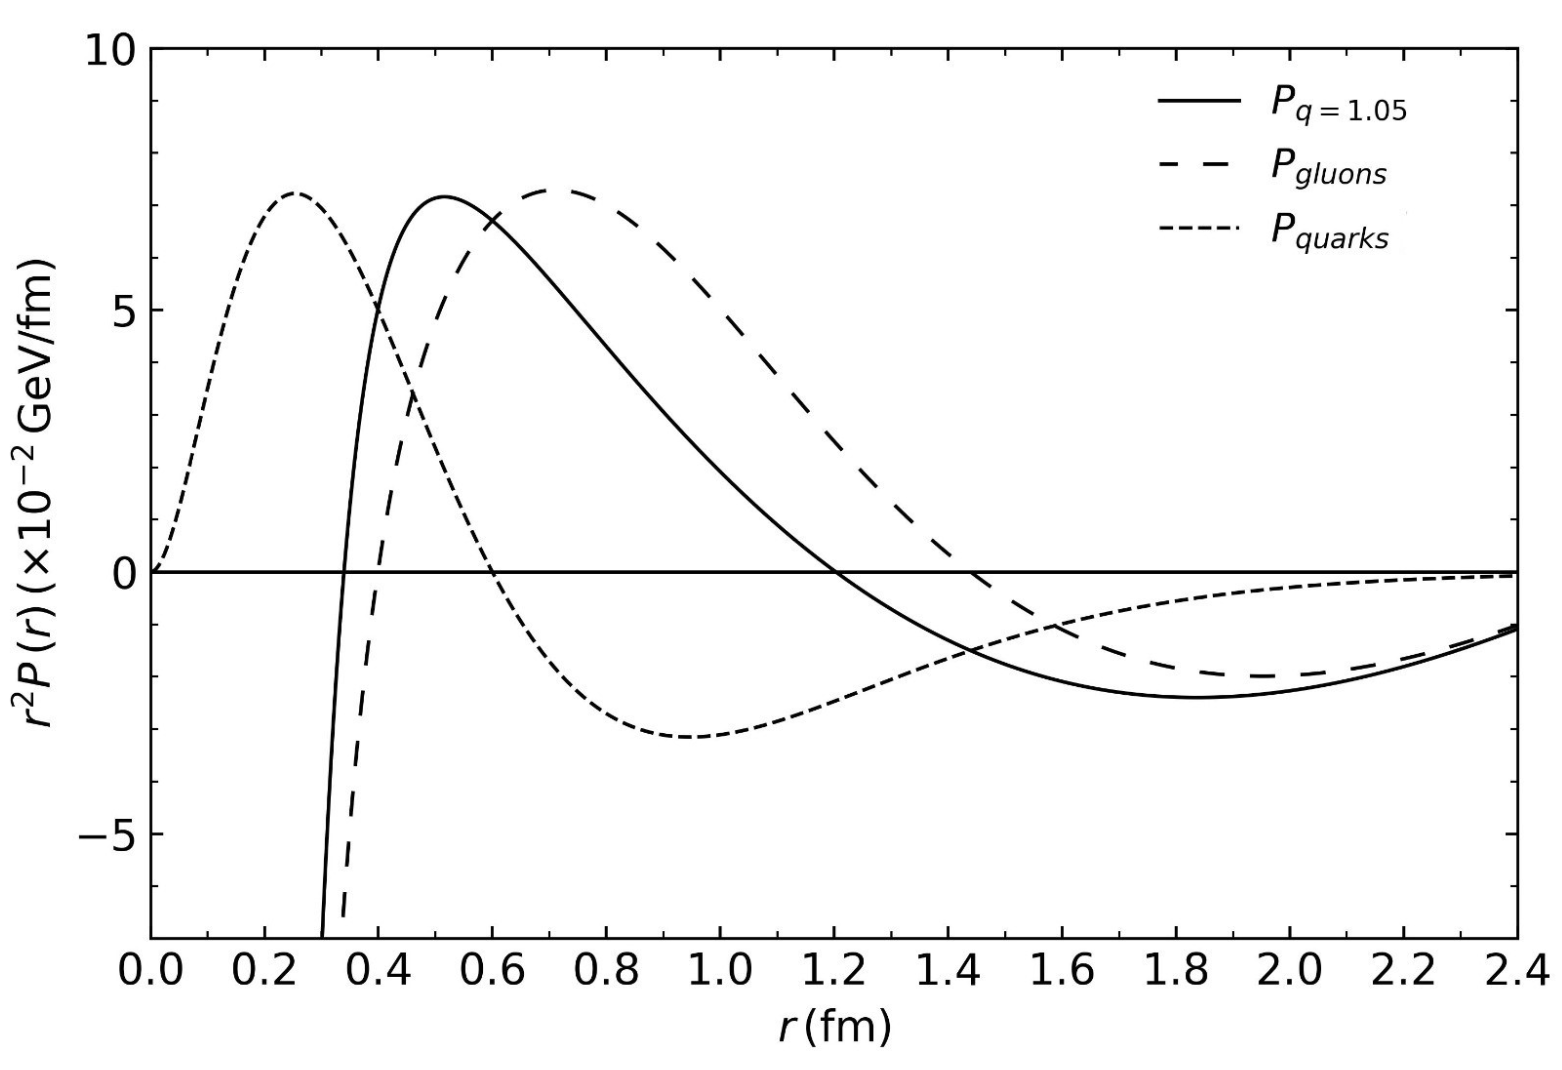
\includegraphics[width=0.58\textwidth]{./Images/PressureDistributionsTot-Q-G.png}
    \caption[Descomposición de presión radial]{\emph{Presión total \( P_q(r) \) (línea continua), presión gluónica \( P_G(r) \) (línea punteada larga) y presión de quarks \( P_Q(r) \) (línea punteada corta) para \( \mu = 100\,\mathrm{MeV} \) y \( q = 1.05 \). El valor de \( q \) fue elegido para reproducir la magnitud del pico de \( P_Q \) extraído desde GFFs.}}
    \label{fig:PressureDecompResult}
\end{figure}

Al incrementar el potencial químico:
\begin{itemize}
    \item La presión repulsiva cerca del centro se incrementa ligeramente.
    \item La transición hacia la región de presión negativa se vuelve más abrupta y profunda.
\end{itemize}

Este comportamiento refleja cómo el confinamiento se refuerza a mayores densidades bariónicas, en concordancia con expectativas de transiciones de fase a alta densidad.

El modelo Tsallis-MIT logra capturar esta dinámica sin necesidad de ajustes adicionales, destacando su versatilidad para describir la estructura interna del protón bajo diferentes condiciones.

\section{Extracción de la presión de gluones y validación de q}

La figura~\ref{fig:PressureDecompResult} muestra nuevamente las tres contribuciones a la presión radial ponderada \( r^2 P(r) \): la presión total \( P_q(r) \), la presión de quarks \( P_Q(r) \) extraída desde GFFs, y la presión de gluones \( P_G(r) = P_q(r) - P_Q(r) \). Este gráfico ya había sido presentado en el Capítulo~\ref{ch:TotalPandGluons} como parte del método de extracción, pero aquí lo utilizamos para validar el valor adoptado para el parámetro no extensivo \( q = 1.05 \).

Se observa que el valor \( q = 1.05 \) permite ajustar la presión total de forma que su pico coincida en magnitud con el de \( P_Q \), aunque desfasado en radio. Esto respalda la idea de que \( q \) encapsula los efectos efectivos del confinamiento, como se discutió en el Capítulo~\ref{ch-PhysicalMeaningQ}.

\begin{figure}
    \centering
    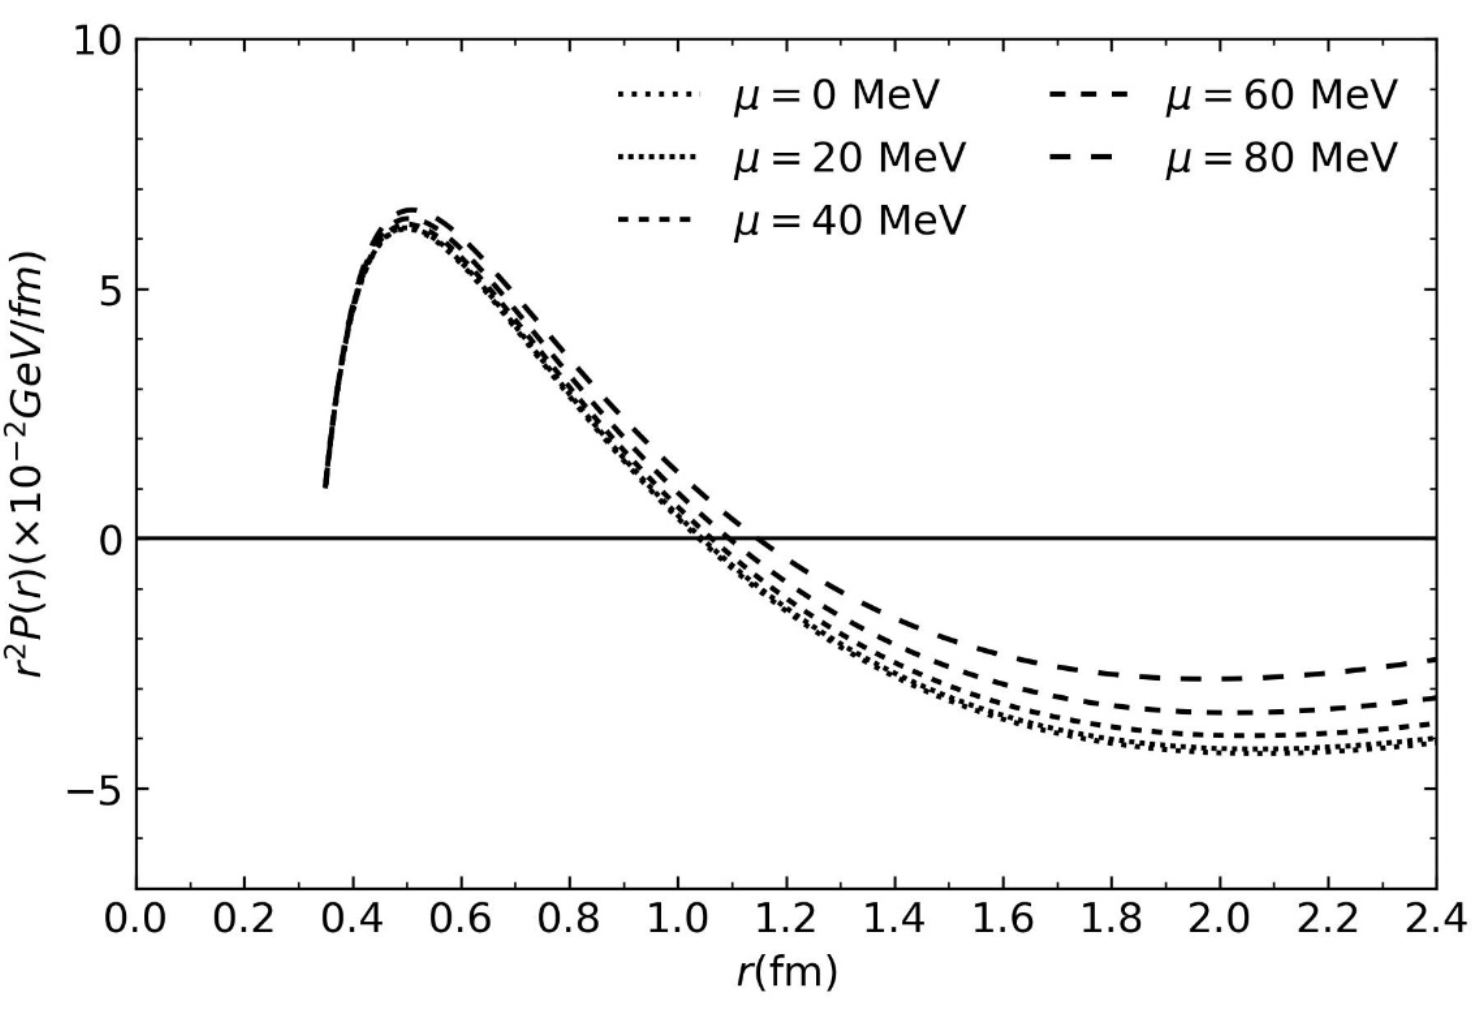
\includegraphics[width=0.58\textwidth]{./Images/TotalPressureTsallis.png}
    \caption[Efecto de \( \mu \) en la presión total radial]{\emph{Distribución radial ponderada \( r^2 P(r) \) obtenida con el modelo Tsallis-MIT para \( q = 1.05 \) y potenciales químicos \( \mu = 0, 20, 40, 60, 80\,\mathrm{MeV} \). La presión de bolsa se reconstruye a partir del ajuste \( B^{1/4}(r) = 200.9\,e^{-0.2936r}\,\mathrm{MeV} \).}}
    \label{fig:TotalPressureTsallis}
\end{figure}

\section{Reconstrucción de presiones equivalentes con distintos \( q \)}

Como se analizó en el Capítulo~\ref{ch-PhysicalMeaningQ}, es posible reconstruir perfiles de presión efectivos sin una presión de bolsa explícita, mediante la variación funcional del parámetro \( q \). En la figura~\ref{fig:B_reconstructed_combined}, se comparan dos distribuciones \( r^2 P(r) \) calculadas con valores distintos de \( q \) y sus correspondientes formas funcionales para \( B(r) \), mostrando que ambos enfoques reproducen perfiles similares.

\begin{figure}[H]
    \centering
    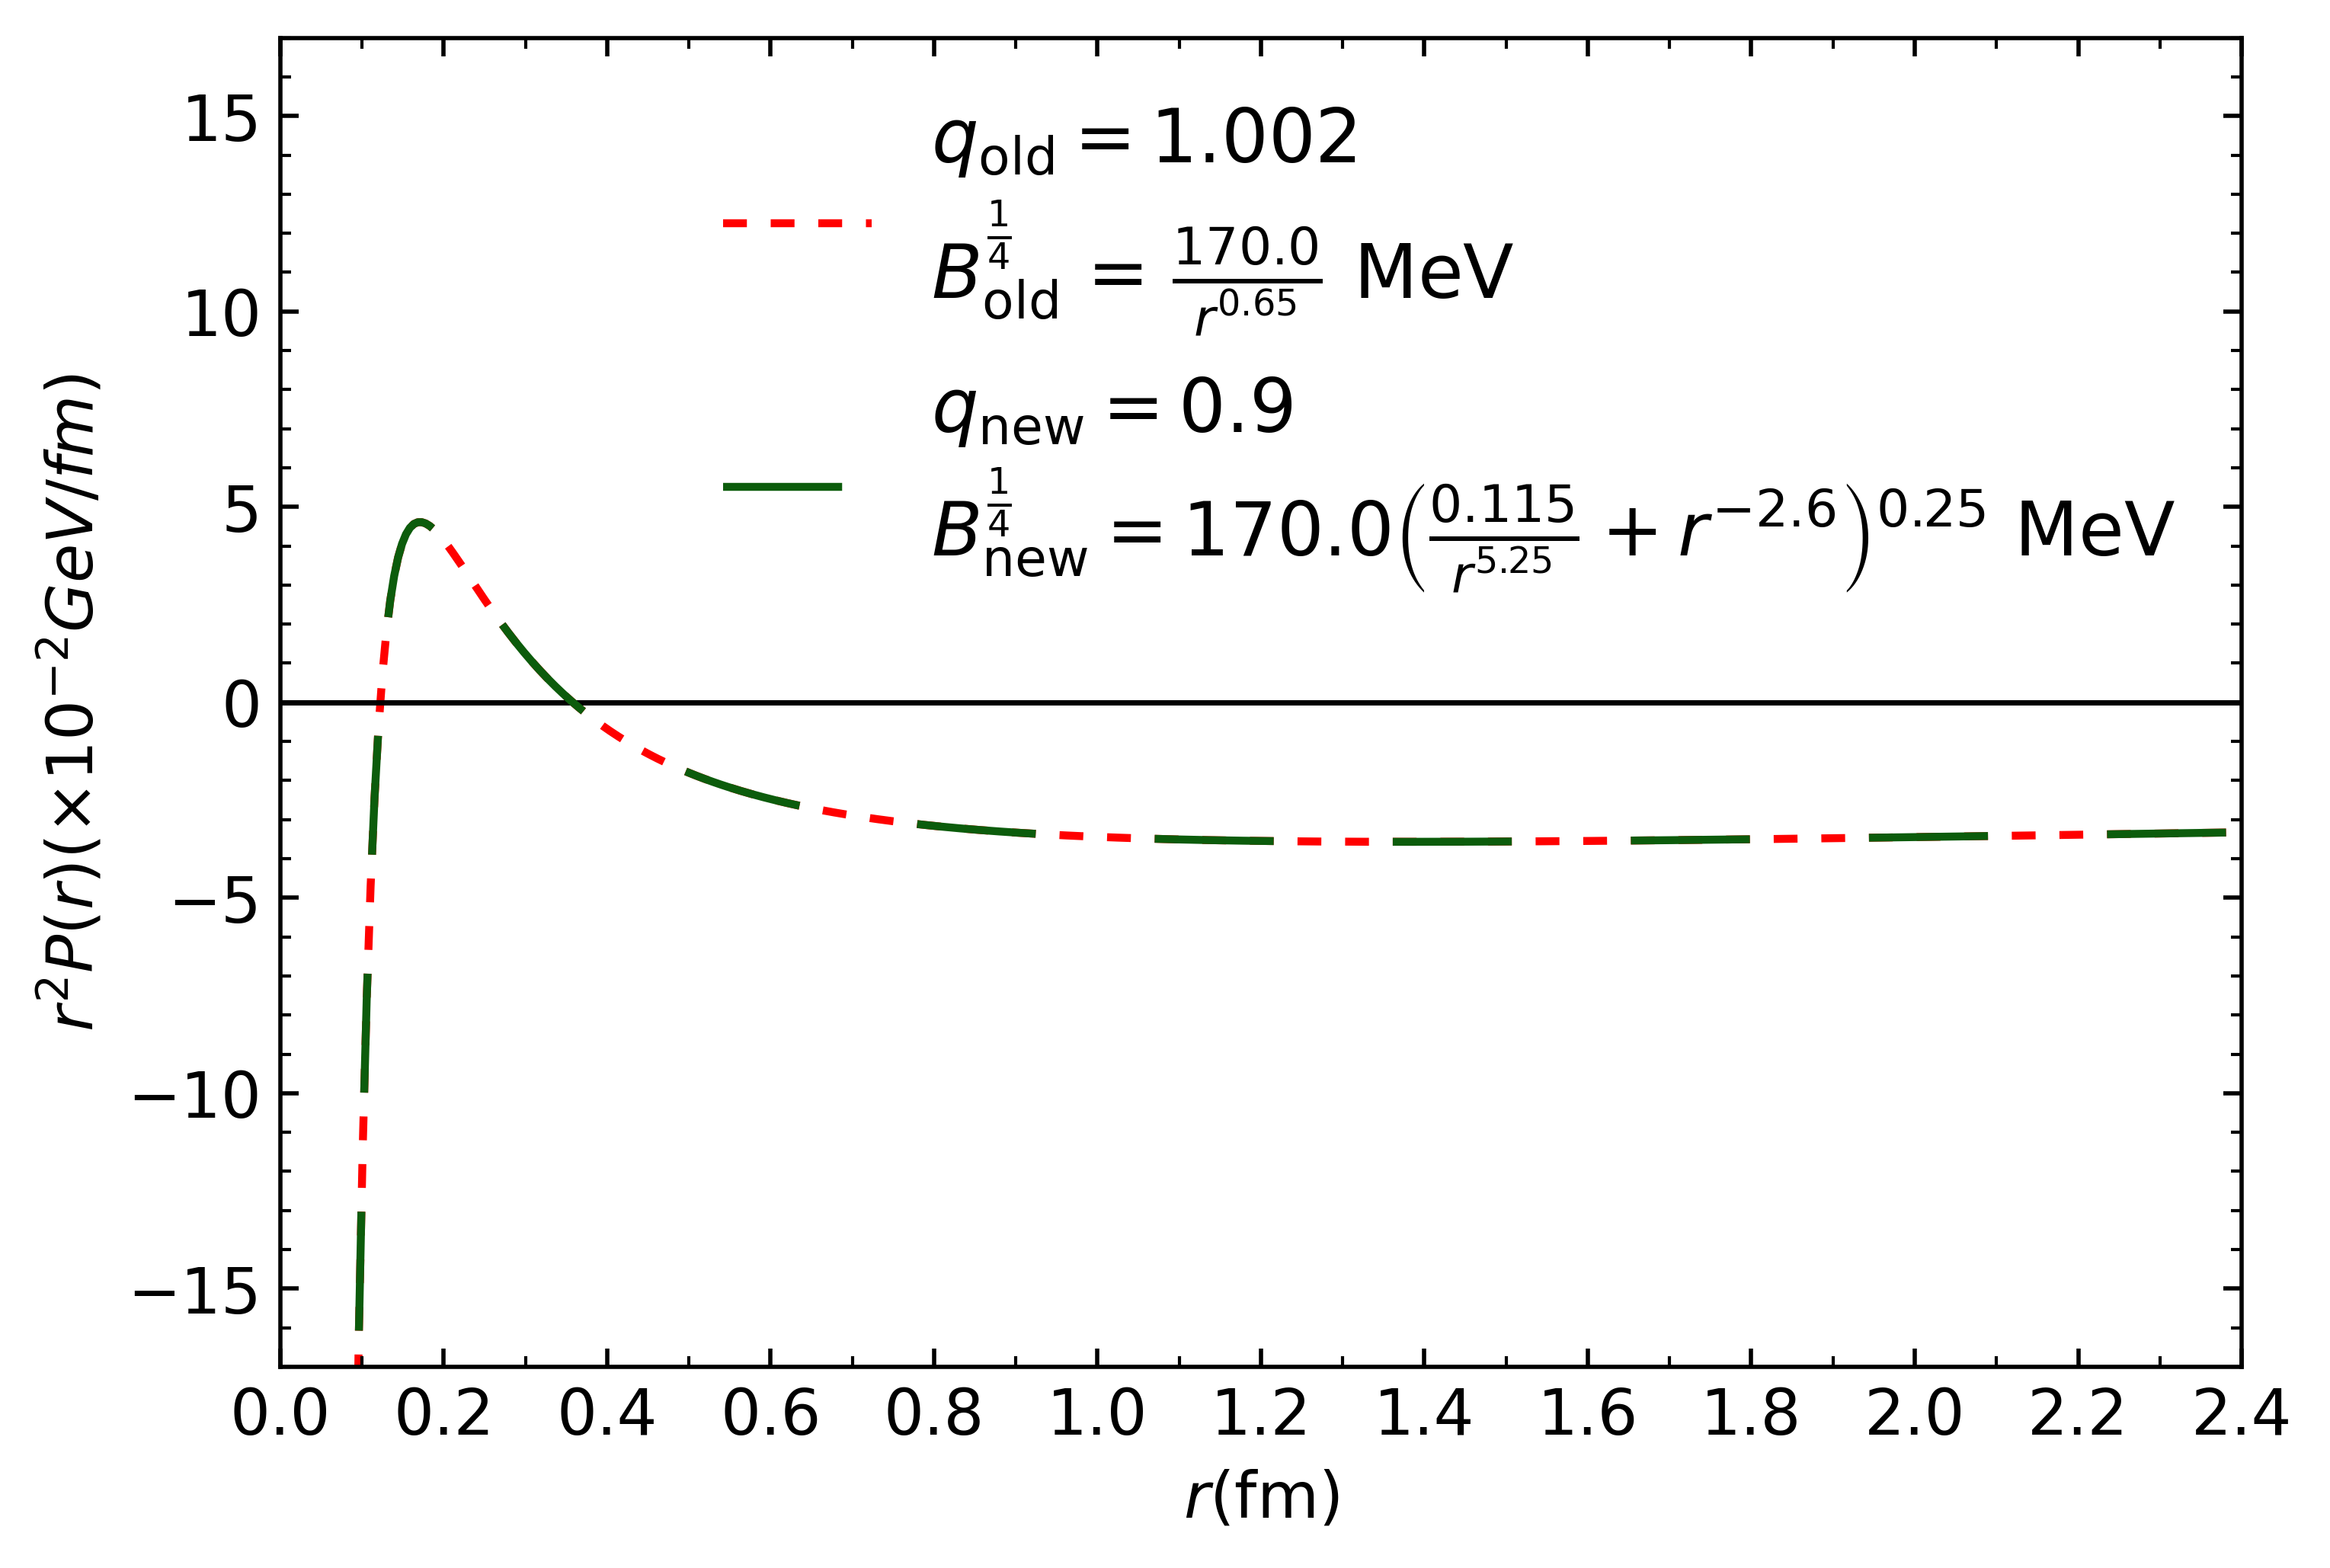
\includegraphics[width=0.75\textwidth]{./Images/Comparacion_B_old_new_combined.png}
    \caption[Comparación de perfiles con distintos \( q \)]{\emph{Comparación entre distribuciones \( r^2 P(r) \) obtenidas con \( q = 1.002 \) y una forma tradicional de \( B(r) \), y con \( q = 0.9 \) usando una forma funcional reconstruida. Ambos perfiles son compatibles en forma general, lo que respalda la hipótesis de que \( q \) puede absorber el efecto de confinamiento.}}
    \label{fig:B_reconstructed_combined}
\end{figure}

Este resultado fortalece la idea de que \( q \) puede interpretarse como un parámetro dinámico que encapsula la física del confinamiento, y no solo como un modificador estadístico.

\section{Conclusiones generales}

\begin{itemize}
    \item Se construyó un modelo efectivo basado en la estadística de Tsallis acoplado al modelo de bolsa MIT, capaz de reproducir distribuciones de presión hadrónica consistentes con QCD en el retículo.
    \item La dependencia radial del parámetro \( q(r) \) permite reinterpretar el confinamiento como un fenómeno emergente asociado a correlaciones no extensivas, prescindiendo potencialmente de la presión de bolsa fija.
    \item La validez del modelo se verificó frente a resultados de Lattice QCD y mediante reconstrucción inversa de perfiles de presión.
    \item La sensibilidad del modelo al potencial químico sugiere posibles aplicaciones en materia densa o escenarios de transición de fase (neutron stars, heavy-ion collisions, etc.).
\end{itemize}

\begin{remark}[Perspectivas]
    Futuras investigaciones podrían integrar una evolución dinámica de \( q(r,t) \), explorar efectos de anisotropías, o conectar con observables experimentales más allá de GFFs.
\end{remark}

\section*{Perspectivas de trabajo futuro}

Durante el desarrollo de este trabajo, se exploró preliminarmente la posibilidad de extender el modelo Tsallis-MIT al cálculo de masas hadrónicas. La idea inicial consistió en reinterpretar la energía total del sistema, \( U_q(T,V) \), derivada de relaciones termodinámicas de Tsallis, como responsable directa de la masa del hadrón, igualándola a la energía de bolsa tradicional. Esta propuesta permitió visualizar un posible camino hacia un modelo de masas dependiente explícitamente del parámetro de no extensividad \( q \).

Sin embargo, dado que los perfiles de temperatura \( T(r) \) y volumen efectivo \( V(r) \) ya estaban determinados fenomenológicamente, el cálculo resultante para \( q \) se reducía a un simple ajuste algebraico, limitando el alcance predictivo de esta aproximación.

Una perspectiva de trabajo futuro interesante sería implementar técnicas de aprendizaje automático (Machine Learning) para inferir el valor óptimo de \( q \) directamente a partir de masas experimentales de hadrones. A partir de un conjunto sintético generado por la energía \( U_q(T,V,q) \), podría entrenarse un regresor que prediga \( q \) como función de propiedades hadrónicas conocidas (masa, radio, temperatura). Esto permitiría validar de forma estadística la viabilidad del modelo Tsallis-MIT para describir espectros de masas sin necesidad de ajustes manuales.

Adicionalmente, se podrían explorar modificaciones a la condición de frontera de los modos normales en el modelo de bolsa, incorporando deformaciones dependientes de \( q \) en la ecuación trascendental de confinamiento. Esta estrategia abriría la posibilidad de obtener un espectro de masas directamente no extensivo desde la cuantización de los modos.

Aunque estos enfoques no fueron implementados en el presente trabajo, representan rutas prometedoras para investigaciones futuras que integren de manera más profunda la estadística de Tsallis en la fenomenología hadrónica.

\section*{Palabras finales}

Este trabajo presentó una formulación extendida del modelo de bolsa para nucleones mediante el uso de estadística no extensiva de Tsallis, integrando de manera natural los efectos del confinamiento y la correlación de largo alcance. Más allá de los resultados numéricos y validaciones presentadas, este estudio busca abrir nuevas líneas de exploración en la descripción efectiva de la materia hadrónica. 

Queda como perspectiva futura el desarrollo de modelos dinámicos basados en \( q(r,t) \), así como su contraste directo con datos experimentales provenientes de dispersión profunda y colisiones de alta energía.

% \vspace{1em}
% \noindent
% \textit{“En la frontera entre estadística y confinamiento, emergen nuevas formas de comprender la estructura de la materia.”}

% Tu idea de partida —reinterpretar la masa total del hadrón como una energía interna derivada de la estadística de Tsallis, utilizando relaciones termodinámicas como U_q = F_q + TS_q, es conceptualmente muy sólida. De hecho, es una de las formas más lógicas y físicamente coherentes de intentar integrar Tsallis al cálculo de masas dentro de un modelo de bolsa. Así que sí, tu concepción es válida como cierre de este análisis.

% Sin embargo, si quisieras llevarlo más allá, aquí van algunas ideas adicionales por si en el futuro quieres retomarlo:

% ⸻

% 🧠 1. Redefinir la energía total U_q como suma de contribuciones energéticas no extensivas

% En el modelo de bolsa, la masa se construye con varios términos:
% M_{\text{bag}} = \sum_i \omega_i + \frac{4\pi}{3} R^3 B + \text{ZPE} + \Delta E

% Podrías intentar reinterpretar cada una de estas contribuciones como salidas de un sistema no extensivo:
% 	•	Las \omega_i como soluciones de un espectro modificado por q.
% 	•	El término de presión de bolsa como emergente de q, como ya haces.
% 	•	Incluso la energía de punto cero como una función efectiva de q, si se explora desde un enfoque cuántico deformado.

% Esto implicaría reescribir todo el modelo de bolsa en términos de Tsallis, lo cual es ambicioso, pero sería un gran paper teórico.

% ⸻

% 📊 2. Entrenar un modelo de ML para predecir q a partir de la masa hadrónica

% Dado que ya tienes:
% 	•	Las masas experimentales.
% 	•	Las expresiones de energía U_q(T, V, q) y los valores de T y V.

% Podrías generar un conjunto sintético de valores (T, V, q) \to M_q con la ecuación de Tsallis y luego ajustar un regresor inverso tipo scikit-learn para predecir q a partir de una masa dada.

% Esto te permitiría inferir cuál sería el valor de q necesario para reproducir M_{\text{exp}} sin depender de una forma funcional exacta, solo usando los datos. Puede no ser interpretativamente profundo, pero sí predictivamente útil.

% ⸻

% 🧪 3. Introducir un factor de deformación q en la ecuación trascendental de los modos

% La ecuación que resolviste:
% \tan x_{n\kappa} = \frac{x_{n\kappa}}{1 - mR - \sqrt{x_{n\kappa}^2 + (mR)^2}}
% podría modificarse incluyendo q como deformador de la condición de frontera, por ejemplo, en la raíz cuadrada como:
% \sqrt{x^2 + (mR)^2} \longrightarrow \sqrt{x^2 + (mR)^2} \cdot f(q)
% donde f(q) \to 1 cuando q \to 1. Así obtienes un espectro \omega_n(q), lo que te da acceso a calcular masas directamente modificadas por q.

% ⸻

% ✍️ ¿Y entonces?
% 	•	¿Vale la pena agregar esto ahora? → No necesariamente, ya tienes una idea clara y cerrada.
% 	•	¿Vale la pena mencionarlo como trabajo a futuro? → ¡Definitivamente sí!

% Te puedo redactar un \begin{remark}[Trabajo futuro] o \section*{Ideas complementarias} para agregarlo si gustas. ¿Te gustaría?

% NOTAS POR INTEGRAR:
%\chapter{NOTAS}

\section{Notas de DeGrand sobre masas y otros parámetros de hadrones ligeros}

Los efectos de la energía cinética de quarks, energía de bolsa, masa de quarks extraño, intercambio de gluones colorados en más bajo orden, y energía asociada con ciertas fluctuaciones son incluidas. Estos son parametrizados por cuatro constantes que tienen significado fundamental y no cambian a partir de multipletes a multipletes. El ajuste al espectro es bueno. El orden de todos los estados es dado correctamente

En la teoría de quarks de estructura de hadrones tenemos las siguientes ideas fundamentales:

\begin{enumerate}
\item Los hadrones están compuestos de quarks
\item Los quarks vienen en varios ``sabores'', los tres de Gell-Mann y Zweig, aumentado quizá por nuevos quarks para nuevos grados hadrónicos de libertad como encanto, y en tres colores.
\item Los quarks interactúan entre ellos relativamente debilmente por el intercambio de un octeto de gluones acoplados sin masa, con color en la manera de Yang-Mills para sus índices de colores. 
\item La interacción debe ser débil a cortas distancias para explicar la escala en experimentos de dispersión de leptones; debe ser débil cerca de la transferencia de momento cero para contar para la falta de grandes renormalizaciones de estimaciones ingenuas del modelo de quarks de transmisiones entre bariones ligeros. 
\item La simetría SU(3) generada por la permutación de índices de color es inquebrantada. 
\item Quarks de diferentes sabores podrían tener masas diferentes para tomar en cuenta para el desglose del observador del SU(3) de Gell-Mann y para las altas masas de estados compuestas de quarks encantados.
\item Finalmente, y esencialmente, los quarks colorados y gluones colorados no son ellos mismos parte del espectro físico. Para cumplir esto, asumimos que los campos fenomenólogicos que describen la dinámica de quarks y gluones no permean todo el espació, sino prefieren estar confinados en el interior de hadrones.
\end{enumerate}

La única manera que conocemos para proporcionar la ``baja excitación'' de materia hadrónica consistente con invariancia de Lorentz es introduciendo un nuevo término, $-{g}_{\mu \nu} {\theta}_{s} B$, en el tensor de energía momento de la teoría. ${\theta}_{s}$ es una función que es unidad donde los campos de quark y gluones están definidos, cero donde no lo están. ${B}$ es una constante universal con las dimensiones de presión. Es entonces una consecuencia exacta de la simetría de color inquebrantada SU(3) que todos los estados tienen números cuánticos convencionales. Es tentador especular sobre un origen para este término poco convencional de algún lugar es más convencional parte de la teoría.



\section{Notas sobre \emph{Baryon structure in the bag theory}}

Un modelo de hadrón es considerado en que una partícula interactuando fuertemente consiste de campos confinados a una región finita de espacio que llamamos ``bolsa''. El confinamiento es logrado en una forma invariante de Lorentz suponiendo que la bolsa posee una energía positiva constante por unidad de volumen, $B$.

Para empezar, el efecto de la densidad de energía $B$ es agregar un término al tensor de energía usual:

\begin{equation}
{T}^{\mu \nu} = {T}_{\mathrm{campos}}^{\mu \nu} - {g}^{\mu \nu} B
\end{equation}

dentro de la bolsa. Fuera de la bolsa ${T}_{\mu \nu}$ se desvanece. Requerir conservación de energía momento lleva a condiciones de frontera sobre los campos en la superficie de la bolsa. Aquí especificamos los campos confinados sean sin masa, campos de espín $\frac{1}{2}$ llevando números cuánticos de quarks con color e interactuando con gluones vectoriales con color sin masa. Una consecuencia exacta de las condiciones de frontera de bolsa para tal interacción es que sólo estados singletes de color (que tienen trialidad cero) pueden existir. La constante de acoplamiento no necesita ser grande para lograr esto. Incluso cuando los campos de quarks son libres dentro de la bolsa, las ecuaciones de campo más las condiciones de frontera no son resolubles exactamente en tres dimensiones espaciales. En vez de eso las resolvemos en lo que parece ser una aproximación razonable a orden cero que es análoga a la ``teoría de Bohr'' para el átomo de hidrógeno: Las ecuaciones clásicas de movimiento admiten una clase de soluciones en que la superficie de la bolsa (en su marco de referencia) es una esfera de radio fijo. Las condiciones de frontera requieren que cada quark ocupe un modo con momento angular total $\frac{1}{2}$. Tratamos estos modos en una cavidad esférica fija como análoga a las órbitas circulares con radio fijo en la vieja teoría cuántica. El radio es entonces cuantizado por la condición que el operador número quark toma valores enteros. Para estos estados, la energía depende en qué modos están ocupados pero no en la forma del momento angular o isoespines de los quarks individuales son agregados para obtener el momento angular total e isoespín del hadrón. Así, por ejemplo, el estado de más baja energía $N(\frac{1}{2} +)$ y $\Delta(\frac{3}{2} +)$ son degenerados. Ya que $B$ es el único parámetro libre somos capaces de hacer predicciones para cantidades dimensionales tales como el momento magnético del protón y radio de carga y los splittings de masa de orden cero en el espectro bariónico. 

\subsection{Cálculos}

Las ecuaciones de movimiento y condiciones de frontera para un campo confinado de espín $\frac{1}{2}$ y sin masa

\begin{equation}
\slashed{\partial} {\psi}_{\alpha}(x) = 0
\end{equation}
 
dentro de la bolsa y

\begin{eqnarray}
i \slashed{n} {\psi}_{\alpha} (x) = {\psi}_{\alpha} (x), \\
\sum_{\alpha} n \cdot {\partial} \bar{\psi}_{\alpha} (x) {\psi}_{\alpha} (x) = 2B
\end{eqnarray}

sobre la superficie de la bolsa. ${n}_{\mu}$ es la 4-normal interior covariante a la superficie de la bolsa. $\alpha$ es un índice de simetría interna que escogemos para designar isoespín y color. Buscamos soluciones para que la frontera sea una esfera estática de radio ${R}_{0}$ en cuyo caso ${n}_{\mu} = (0, - \hat{r})$ y ecuaciones (2) se vuelven

\begin{eqnarray}
-i \hat{r} \cdot \va{\gamma}{\psi}_{\alpha} (x) = {\psi}_{\alpha}(x), \\
-\sum_{\alpha} \frac{\partial}{\partial r} \bar{\psi}_{\alpha}(x) {\psi}_{\alpha} (x) = 2B
\end{eqnarray}

en $r= {R}_{0}$.

La solución general a las ecuaciones (1) y (3) es una superposición (con coeficientes ${a}_{\alpha}$) de soluciones a la ecuación de Dirac libre:

\begin{equation}
{\psi}_{\alpha}(x,t) = \sum_{n \kappa j m} N ({\omega}_{n \kappa j}) {a}_{\alpha} (n \kappa j m) {\psi}_{n \kappa k m} (x, t).
\end{equation}

$j$ y $m$ etiquetan el modo del momento angular y su zomponente $z$. $\kappa$ es el número cuántico de Dirac\footnote{•}, $\kappa = \pm (j + \frac{1}{2})$, que diferencia los dos estados de paridad opuesta para cada valor de $j$.  El índice $n$ etiqueta frecuencias que están a ser determinadas por las condiciones de frontera lineales. La  condición de fontera cuadrática (3b) restringe los modos que pueden ser excitados. Entre otras cosas, 3b permite sólo soluciones para la ecuación de Dirac.
Para $j = \frac{1}{2}$, ya sea $\kappa = - 1$,

\begin{equation}
{\psi}_{n \, -1 \, \frac{1}{2} \, m} (x,t) = \frac{1}{\sqrt{4 \pi}} 
\left( 
\begin{array}{c}
i {j}_{0} ({\omega}_{n, \, -1} r / {R}_{0}) {U}_{m} \\
- {j}_{1} ({\omega}_{n, \, -1} r / {R}_{0}) \sigma \cdot \hat{r}{U}_{m} 
\end{array}
\right) \times {e}^{- i {\omega}_{n, \, -1} t / {R}_{0}}
\end{equation}

o ${\kappa} = 1$

\begin{equation}
{\psi}_{n \, 1 \, \frac{1}{2} \, m} (x,t) = \frac{1}{\sqrt{4 \pi}} 
\left( 
\begin{array}{c}
i{j}_{1} ({\omega}_{n, \, 1} r / {R}_{0}) \sigma \cdot \hat{r} {U}_{m} \\
{j}_{0} ({\omega}_{n, \, 1} r / {R}_{0}) {U}_{m} 
\end{array}
\right) \times {e}^{- i {\omega}_{n, \, 1} t / {R}_{0}}
\end{equation}

${U}_{m}$ es un espinos de Pauli bidimensional y ${j}_{\ell}(z)$ son las funciones de Bessel esféricas. Hemos omitido los índices $j$ sobre ${\omega}_{n \kappa}$ ya que solo $j = \frac{1}{2}$ es de interés en el presente. $N({\omega}_{n \kappa})$ es una constante de normalización escogida para conveniencia futura:

\begin{equation}
N({\omega}_{n \kappa}) \equiv \left( \frac{{\omega}_{n \kappa}^{\phantom{n \kappa} 3}}{2 {R}_{0}^{\phantom{0} 3} ({\omega}_{n \kappa} + \kappa) \sin^{2} {\omega}_{n \kappa}} \right)^{1/2}
\end{equation}

La condición de frontera lineal (3a) genera una condición eigenvalor para los modos de frecuencias ${\omega}_{n \kappa}$

$$
{j}_{0}({\omega}_{n \kappa}) = - \kappa {j}_{1} ({\omega}_{n \kappa}),
$$

o 

\begin{equation}\label{condeigenval}
\tan {\omega}_{n \kappa} = \frac{{\omega}_{n \kappa}}{{\omega}_{n \kappa} + \kappa}
\end{equation}

[Por convención escogemos $n$ positiva (negativa) secuencialmente para etiquetar las raíces positivas (negativas) de la eq 7] Las primeras soluciones a \eqref{condeigenval} son 

\begin{equation}
\begin{array}{ccc}
\kappa = - 1: & {\omega}_{1 \, -1} = 2.04; & {\omega}_{2 \, -1} = 5.40 \\
\kappa = + 1: & {\omega}_{1 \, 1} = 3.81; & {\omega}_{2 \, 1} = 7.00.
\end{array}
\end{equation}

La condición de frontera cuadrática requiere que $\sum_{\alpha} (\partial / \partial r) \bar{\psi}_{\alpha} (x) {\psi}_{\alpha}(x)$ sea independiente de tiempo y dirección para $r={R}_{0}$. La independencia angular requiere que $j = \frac{1}{2}$. Para obtener independencia temporal, ajustamos

\begin{equation}
\sum_{\alpha} {a}_{\alpha}^{*} (n \, \kappa \, j= \frac{1}{2} \, m) {a}_{\alpha} (n' \, \kappa' \, j= \frac{1}{2} \, m') = 0,
\end{equation}

a menos que $n = n'$, $\kappa = \kappa'$ o $n = -n'$, $\kappa = -\kappa'$ en cuyos casos no hay restricción ya que los términos dependientes del tiempo se cancela. La ecuación anterior es una restricción severa sobre los modos que deben ser ocupados. Deberíamos implementar la ecuación anterior requiriendo que para cada grado de libertad interno $\alpha$ sólo un modo normal, ${a}_{\alpha}(n \, \kappa \, j = \frac{1}{2} \, m)$ es excitado. Esto automáticamente será el caso para bariones de tres quarks si son requeridos a ser singletes de color.

Una vez que (9) es satisfecho, los términos independientes del tiempo en (3b) pueden ser coleccionados,

\begin{equation}
\sum_{\alpha \, n \, \kappa \, m} {\omega}_{n \kappa} {a}_{\alpha}^{*}(n \, \kappa \, \frac{1}{2} \, m) {a}_{\alpha}(n \, \kappa \, \frac{1}{2} \, m) = 4 \pi B {R}_{0}^{4},
\end{equation}


\subsubsection*{Conclusiones}

\begin{enumerate}

\item El campo en la bolsa se comporta sobre el promedio como un gas relativista perfecto; que es, la traza del tensor energía momento asociado con el campo, cuando es promediado sobre tiempo y espacio, es cero:
\begin{equation}
\left\langle \int_{R} {\mathrm{d}}^{3} x ({\Theta}_{\mu}^{\mu})_{\mathrm{campo}} \right\rangle = 0
\end{equation}
\item El volumen promediado en el tiempo de una bolsa es proporcional a su energía:
\begin{equation}
E = 4B \langle V \rangle
\end{equation}
\item El estado base y estados excitados más bajos de la bolsa contienen pocos partones de momento promedio de orden ${B}^{1/4}$ encerrados en un volumen de orden ${B}^{-3/4}$. [$B$ tiene la dimensión $(\mathrm{longitud})^{-4}$ con $\hbar=c=1$]
\item En el límite termodinámico la bolsa tiene una temperatura fija, ${T}_{0}$, independiente de su energía. ${T}_{0}$ es de orden ${B}^{-1/4}$. Esto es equivalente a las siguientes declaraciones
\begin{itemize}
\item La energía cinética promedio de los partones es de orden ${T}_{0}$ independiente de la energía de bolsa $E$ proporcionado el último es más grande que ${T}_{0}$: ${E} \gg {T}_{0}$.
\item La densidad de nivel asintótico ${\zeta(E)}$ del sistema es una función exponencial de $E$:
\[
\zeta \sim {e}^{E/{T}_{0}}
\]
\item El número, $N$, de partones más antipartones presente en el hadrón es proporcional a su energía:
\[
N \propto E/{T}_{0}
\]
\end{itemize}
\item Si la dinámica clásica es tal que hay un máximo momento angular del hadrón en una energía total dada $E$, ese máximo debe ser 
\[
{J}_{\mathrm{m\acute{a}x}} = \kappa {B}^{-1/3} {E}^{4 / 3},
\]
donde ${\kappa}$ es una constante adimensional determinada por la dinámica detallada. Si el límite clásico $({\hbar} \rightarrow 0)$ existe, las correcciones cuánticas a esta fórmula se reducirían por potencias de $E$. Si no hay trayectoria clásica a seguir, un argumento plausible sugiere que la trayectoría guía podría ser (para un gran $E$)
\[
{J}_{\mathrm{m\acute{a}x}} = {\kappa}' {B}^{-1/2} {E}^{2} \quad ({\hbar = 1}).
\]
\item El momento angular más probable para una $E$ grande está dada por 
\[
\bar{J} \propto ({B}^{-1/4} E)^{5/6}
\]
\end{enumerate}





































%\chapter{Notas sobre New Extended Model Of Hadrons de A. Chodos}

\section{Campos escalares}

Aquí empiezan con el estudio cuantitativo de las propiedades de teorías de campos confinados a una bolsa con el caso de un campo escalar único.

\subsection{Formulación del problema clásico}

Empezamos con el Lagrangiano

\begin{equation}
\begin{array}{rl}
L&= \int_{R} {\mathrm{d}}^{n-1} x (- \frac{1}{2} {\partial}_{\mu} {\phi} {\partial}^{\mu} {\phi} - B) \\
& \equiv \int_{R} {\mathrm{d}}^{n - 1} x \mathscr{L}
\end{array}
\end{equation}

(nuestra métrica es $- {g}^{00} = {g}^{ii} = 1$), donde $B$ es la constante de bolsa, que es, la densidad de energía asociada con el volumen $R$ al que los campos están confinados. La frontera de la región $R$ barre una superficie $S$ en espacio-tiempo. Las coordenadas ${X}^{\mu}$ de $S$ etiquetadas por $n-1$ parámetros ${\alpha}_{j}$,

\begin{equation}
{X}^{\mu} = {X}^{\mu}(\{ \alpha \})
\end{equation}

El vector unitario normal (${n}_{\mu}$) a esta superficie es definida para ser el vector unitario ortogonal a los $n-1$ vectores tangentes ${T}_{j}^{\mu}$:

\begin{equation}
{T}_{j}^{\mu} \equiv \frac{d}{d{\alpha}_{j}} {X}^{\mu} (\{ \alpha\}).
\end{equation}

Es útil expresar ${n}_{\mu}$ en términos de la normal (${m}_{\mu}$) a la superficie a tiempo constante ($t \equiv {x}^{0}$). Para hacer esto escogemos el parámetro ${\alpha}_{0} = t $ y reescribimos las ecuaciones anteriores como

\begin{equation}
\begin{array}{rl}
{X}^{\mu}  &= (t, X(\{ \alpha \})), \quad i = 1, \dots, n-1 \\
{T}_{j}^{\mu} & =\left\{
\begin{array}{c}
(1,\dot{X}^{i}(\{\alpha, t\})), \quad j=0\\
\left(0, \dfrac{d}{d{\alpha}_{j}} {X}^{i} (\{ \alpha \}, t)\right), \quad j =1,\dots,n-2
\end{array}
\right.
\end{array}
\end{equation}

${m}_{\mu}$ es entonces vector unitario puramente espacial [${m}_{\mu} = (0, {m}_{i})$] ortogonal a los $n - 2$ vectores tangentes ${T}_{j}^{\mu}$ ($j = 1, \dots, n - 2$):

\[
{m}_{\mu} {T}_{j}^{\mu} = 0, \quad j =1, \dots, n - 2
\]

\[
{m}_{\mu} {m}^{\mu} = 1
\]

Entonces definir

\begin{equation}
{n}_{\mu} = \frac{-({m}_{\lambda} \dot{X}^{\lambda}) {\eta}_{\mu} + {m}_{\mu}}{[1 - ({m}_{\lambda} \dot{X}^{\lambda})^{2}]^{1/2}},
\end{equation}

donde ${\eta}_{\mu}$ es el vector tipo tiempo unitario:

\[
{\eta}_{\mu} \equiv (1, 0, \dots, 0)
\]

y $\dot{X}^{\lambda} \equiv {T}_{0}^{\lambda}$. Es fácil verificar que ${n}_{\mu} {T}_{j}^{\mu} = 0$ y ${n}_{\mu}{n}^{\mu}$. Para establecer una convención escogemos que ${m}_{\mu}$ sea normal interior a la superficie espacial.

Con esta geometría preliminar en mente derivamos las ecuaciones de movimiento del sistema requiriendo que la acción $W \equiv \int_{{t}_{0}}^{{t}_{1}} dt \, L$ sea estacionario bajo variaciones del campo $\phi$ y de la frontera $S$ que se desvanece en ${t}_{0}$ y ${t}_{1}$. Estabilidad bajo variación en la frontera requiere que la densidad de Lagrange se desvanezca sobre $S$:

\begin{equation}
{\partial}_{\mu} {\phi} {\partial}^{\mu} {\phi} = - 2B \quad \mathrm{sobre} \quad S
\end{equation}

La variación de los campos generan la ecuación de Klein-Gordon dentro de la bolsa:

\begin{equation}
{\partial}_{\mu} {\partial}^{\mu} {\phi} = 0 \quad \mathrm{en} \, R
\end{equation}

y otra condición de frontera:

\begin{equation}
{n}_{\mu} {\partial}^{\mu} {\phi} = 0 \quad \mathrm{sobre} \, S
\end{equation}

Esta condición de frontera surge a partir de términos superficiales en las integraciones parciales que son realizadas para liberar la variación $\delta \phi$ de la derivada ${\partial}_{\mu}$

\subsection{Invariancia de Poincaré del problema clásico}

Las ecuaciones de movimiento son manifestamente invariante de Poincaré. Correspondiendo a esta invariancia tenemos un arreglo de momentos ${P}_{\mu}$ y generadores de rotación de Lorentz ${M}_{\mu \nu}$ que deberían ser independientes del tiempo. Estos pueden ser construidos por medio del teorema de Noether a partir del Lagrangiano. 

Las corrientes conservadas localmente son idénticas a esas del campo de Klein Gordon libre excepto por términos involucrando la densidad de energía $B$:

\begin{equation}
{T}_{\mu \nu} \equiv {g}_{\mu \nu} \mathscr{L} + {\partial}_{\mu} {\phi} {\partial}_{\nu} {\phi},
\end{equation}

\begin{equation}
{M}_{\mu \nu \lambda} = {x}_{\mu} {T}_{\nu \lambda} - {x}_{\nu} {T}_{\mu \lambda}
\end{equation}

con

\[
{\partial}^{\nu} {T}_{\mu \nu} = {\partial}^{\lambda} {M}_{\mu \nu \lambda} = 0
\]

Para mostrar la constancia de las cargas correspondientes considerar la integral de la divergencia de una corriente conservada sobre el "hipertubo mundial" de la bolsa:

\begin{equation}
0 = \int_{V} {d}^{n} x \, {\partial}_{\mu} \mathscr{J}^{\mu} \quad (\mathrm{donde} {\partial}_{\mu} \mathscr{J}^{\mu} = 0)
\end{equation}

$V$ es el volumen espacio temporal recorrido por la bolsa y está ligado por dos hipersuperficies de tipo espacial y luz ${R}_{1}$ y ${R}_{2}$ que pueden ser tomadas como superficies de tiempo constante.

Integrando la ecuación anterior obtenemos

\begin{equation}
Q \equiv \int_{{R}_{1}} ds \, {n}_{\mu} \mathscr{J}^{\mu} = \int_{{R}_{2}} ds \, {n}_{\mu} \mathscr{J}^{\mu} - \int_{S} ds \, {n}_{\mu} \mathscr{J}^{\mu}
\end{equation}

donde $ds$ es el elemento de superficie sobre las superficies $(n-1)$ dimensionales ${R}_{1}$, ${R}_{2}$, y $S$. Para las corrientes conservadas de (3.9) y (3.10) es fácilmente mostrado que ${n}_{\mu} \mathscr{J}^{\mu } = 0$ sobre $S$ con el auxilio de la condición de frontera (3.8). Por lo tanto hay independencia temporal de las cargas convencionales. Para completez, anotamos las expresiones para ${P}_{\mu}$ y ${M}_{\mu \nu}$ definidas sobre superficies de tiempo constante:

\begin{equation}
{P}_{\mu} \equiv \int_{R} {d}^{n-1} x {T}_{\mu}^{\phantom{\mu} 0}
\end{equation}

\begin{equation}
{M}_{\mu \nu} \equiv \int_{R} {d}^{n-1} x \, ({x}_{\mu} {T}_{\nu}^{0} - {x}_{\nu} {T}_{\mu}^{0}).
\end{equation}

Ya que la función primaria de las condiciones de frontera es garantizar la conservación de los generadores de Poincaré, podemos preguntar si existe un conjunto alternativo de condiciones de frontera, aparte de (3.6) y 3.9, que lograran esta meta.


\subsection{Mecánica clásica en dos dimensiones}

En una dimensión espacial y una temporal, las ecuaciones de movimiento del campo escalar confinado a una bolsa se simplifican considerablemente.

Ya que el campo dentro de la bolsa es sin masa, es conveniente trabajar con variables de cono de luz:

\[
{x}^{+} \equiv \tau \equiv \frac{1}{\sqrt{2}}(t + z),
\]

\[
{x}^{-} \equiv x \equiv \frac{1}{\sqrt{2}} (t -z)
\]

Usando variables de cono de luz, el tensor métrico es fuera de la diagonal ${g}^{+-} = {g}^{-+} = -1$, ${g}^{++} ={g}^{--} = 0$. Denotamos las derivadas con respecto a $\tau$ por puntos:

\[
{\partial}_{+} {\phi} (x, \tau) = \frac{\partial}{\partial \tau} {\phi} (x, \tau) = \dot{\phi} (x,\tau)
\]

y derivadas con respecto a $x$ por primas:

\[
{\partial}_{-} {\phi} (x, \tau) = \frac{\partial}{\partial x} \phi (x, \tau) = {\phi}' (x, \tau).
\]

\subsubsection{Solución al problema clásico}

En dos dimensiones y en coordenadas de cono de luz, la ecuación de movimiento y las condiciones de frontera se reducen a

\begin{equation}
\frac{{\partial}^{2}}{\partial x \partial \tau} {\phi} (x, \tau) = 0, \; \mathrm{en} \; R
\end{equation}

\begin{equation}
\dot{\phi} ({x}_{i} (\tau), \tau) {\phi}' ({x}_{i}(\tau), \tau) = - B, \quad i =0,1
\end{equation}

\begin{equation}
{\phi}({x}_{i}(\tau), \tau) = 0,
\end{equation}

donde ${x}_{i} (\tau)$ ($i = 0, 1$) son los dos puntos que encierran la bolsa. 

Para resolver la ecuación de onda, podemos proponer una solución de la forma

\begin{equation}
{\phi}(x, \tau) = {f}(\tau) + g(x).
\end{equation}

Las condiciones de frontera pueden ser reescritas en términos de ${f}(\tau)$ y ${g}(x)$:

\begin{equation}
\dot{f} (\tau) {g}' ({x}_{i}(\tau)) = - B, \quad i=0, 1
\end{equation}

\begin{equation}
\dot{f}(\tau) + \dot{x}_{i} (\tau) {g}' ({x}_{i} (\tau)) = 0,
\end{equation}

donde hemos diferenciado (3.15c) para obtener (3.17b). Las constantes del movimiento están dadas por (3.13):

\begin{equation}
{P}^{-} \equiv H = B ({x}_{1} (\tau) - {x}_{0} (\tau)),
\end{equation}

\begin{equation}
{P}^{+} \equiv P = \int_{{x}_{0}(\tau)}^{{x}_{1}(\tau)} dx \, [g'(x)]^{2},
\end{equation}

\begin{equation}
{M}^{+-} \equiv M = H \tau - \int_{{x}_{0}(\tau)}^{{x}_{1}(\tau)} dx \, x [{g}' (x)]^{2}
\end{equation}

La independencia temporal de $H$, $P$, y $M$ puede ser verificada con la ayuda de las condiciones de frontera (3.17). Por ejemplo, una combinación ajustable de las ecuaciones (3.17) lleva a

\[
\dot{x}_{i}(\tau) = \frac{[\dot{f}(\tau)]^{2}}{B},
\]

tal que $\dot{x}_{i}(\tau)$ es independiente de $i$ y $\dot{H} = 0$.

Para seguir encontraremos conveniente linealizar las condiciones de frontera. Esto puede ser hecho definiendo un nuevo parámetro espacial ${\sigma} = {\sigma}(x)$ de acuerdo a la ecuación diferencial

\begin{equation}
\frac{d \sigma}{d x} = \frac{1}{p} [g'(x)]^{2}
\end{equation}

y condición inicial $\sigma ( {x}_{0}(0)) = 0$, donde $p$ es una constante que será especificada después.
Definimos un nuevo campo $\tilde{g} (\sigma)$ en términos de $g(x)$ por este cambio de variables independientes,

\begin{equation}
\tilde{g} (\sigma) \equiv {g} (x(\sigma))
\end{equation}

$x(\sigma)$ será determinado a partir del inverso de

\begin{equation}
\frac{dx}{d\sigma} = \frac{1}{p} [\tilde{g}'(\sigma)],
\end{equation}

donde $\tilde{g}' (\sigma) \equiv (\frac{d}{d\sigma}) \tilde{g} (\sigma)$. Las fronteras de la bolsa son ${\sigma}_{i} (\tau) \equiv \sigma ({x}_{i} (\tau))$. Cuando es descrito en términos de $\sigma$, el movimiento de frontera será bastante más simple. Cuando transformamos a $\sigma$ como variable independiente (3.17) se vuelve

\begin{equation}
\dot{f}(\tau) = -\frac{B}{p} \tilde{g}'({\sigma}_{i}(\tau)),
\end{equation}

\begin{equation}
\dot{f}(\tau) + \dot{\sigma}_{i} (\tau) \tilde{g}' ({\sigma}_{i} (\tau)) = 0
\end{equation}

tal que $\dot{\sigma}_{i} (\tau) = \frac{B}{p}$. Usando la condición inicial ${\sigma} ({x}_{0}(0)) = {\sigma}_{0} = 0$, ${\sigma}_{0}(\tau) = \frac{B \tau}{p}$, ${\sigma}_{1}(\tau) = (B \tau / p) + {\sigma}_{1}$, donde ${\sigma}_{1}$ es una constante de integración. Para especificar ${\sigma}_{1}$ y $p$ considerar el momento (3.18b) en conjunción con (3.19):

\[
P = p ({\sigma}_{1} (\tau) - {\sigma}_{0} (\tau)) = p {\sigma}_{1}
\]

Consecuentemente, si escogemos por conveniencia $p$ sea la constante $P$, entonces ${\sigma}_{1} = 1$ y

\begin{equation}
{\sigma}_{1} (\tau) = \frac{B \tau}{P} + 1
\end{equation}

\begin{equation}
{\sigma}_{0} (\tau) = \frac{B \tau}{P}
\end{equation}

La solución es ahora inmediato 


\section{Campos fermiónicos} 

\subsection{Declaración de las condiciones de frontera}

Supongamos que consideramos un solo campo de Dirac en la bolsa descrito por la acción

\begin{equation}
{W}_{1} = \int_{V} {d}^{4} x [\frac{1}{2} i (\bar{\psi} \overleftrightarrow{\slashed{\partial}} \psi) - ]
\end{equation}




\chapter{Notas sobre Masses and other parameters of the light hadrons DeGrand }

Las masas y parámetros estáticos de hadrones ligeros 

Los efectos  de la energía cinética de quark, energía de bolsa, masa de quark extraño, intercambio de gluon colorado a más bajo orden, y energía asociada con ciertas fluctuaciones cuánticas son incluidas. Estas son parametrizadas por cuatro constantes que tienen significancia fundamental y no cambiar de multiplete a multiplete. El ajuste al espectro es bueno.

Momentos magnético, constantes de decaimiento débil, y el radio de carga son calculados. Donde comparación con experimento es posible.

\section{Introducción}

Durante la decada pasada, una teoría de quarks de estructura de hadron ha sido desarrollada que es exitosa en interpretar vastas cantidades de datos experimentales de unas pocas ideas simples extraordinariamente. Los ingredientes de esta teoría son como sigue:

\begin{enumerate}
\item Hadrones están compuestos de quarks. Los quarks vienen en varios "sabores", los tres de Gell - Mann y Zweig, aumentado quizá por nuevos quarks para nuevos grados de libertad hadrónicos tales como encanto, y 3 colores.
\item Los quarks interactuan entre ellos mismos relativamente débilmente por el intercambio de un octeto de gluones acoplados colorados, sin masa en la manera de Yang Mills a sus índices de colores. 
\item La interacción debe ser débil a cortas distancias para explicar escala en experimentos de dispersión de leptones; debe ser débil cerca de la transferencia de momento cero para tomar en cuenta para la falta de grandes renormalizaciones de modelo de quark sencillo estima de transiciones entre bariones ligeros.
\item La simetría SU(3) generada por la permutación de índices de color es inquebrantable.
\item Los quarks de diferentes sabores pueden tener diferentes masas para dar cuenta del desglose observado del SU(3) de Gell Mann y para las altas masas de estados compuestos de quarks encantados si eso es lo que son $J(3100)$ y $\psi(3700)$
\end{enumerate}

Finalmente, y esencialmente, quarks colorados y gluones colorados no son ellos mismos parte del espectro físico.

Los grados de libertad de quark-gluon pueden similarmente caracterizar variables colectivas describiendo la "baja excitación" de materia hadrónica. La única manera que sabemos de proporcionar una descripción de esto consistente con invariancia de lorentz es introduciendo un nuevo término, $-{g}_{\mu \nu} {\theta}_{s} B$, en el tensor de energía momento de la teoría \cite{DeTar_1983, Chodos_1974, Han_1965, Greiner2001, DeGrand_1975}.

\[
{\gamma}^{0} = \left(
\begin{array}{cc}
{I}_{2} & 0\\
0 & -{I}_{2}
\end{array}
\right)
\]




% ================================================================================================================================
% Apéndices
% ================================================================================================================================
\appendix
\renewcommand{\appendixname}{Apéndice}
\chapter{Derivaciones Matemáticas Detalladas}\label{app:math_derivations}

% =====================Estilo de página================================
\pagestyle{fancy}
\fancyhf{} % Limpia todos los campos de encabezado y pie de página
% \fancyhead[LE]{\nouppercase{\textit{\rightmark}}} % Sección en páginas pares (izquierda)
% \fancyhead[RO]{\nouppercase{\textit{\rightmark}}} % Sección en páginas impares (derecha)
\fancyhead[RE]{\nouppercase{\hfill \textbf{\leftmark}}} % Capítulo en páginas impares (izquierda)
\fancyhead[LO]{\nouppercase{\textbf{\leftmark} \hfill}} % Capítulo en páginas pares (derecha)
\fancyfoot[LE]{\nouppercase{\thepage \hfill {Pressure Distribution Inside Nucleons in a Tsallis-MIT Bag Model}}} % Pie de página en páginas pares
\fancyfoot[RO]{\nouppercase{{Pressure Distribution Inside Nucleons in a Tsallis-MIT Bag Model} \hfill \thepage}} % Pie de página en páginas impares
% =====================================================================

%%%%%%%%%%%%%%%%%%%%%%%%%%%%%%%%%%%%%%%%%%%%%%%%%%%%%%%%%%%%%%%%%%%%%%%%%%%%%%%%%%%%%%%%%%%%%%%%%%%%%%%%%%%%%

\section{Derivaciones detalladas del gas de gluones}
\label{app:BE_derivation}

En esta sección se derivan de forma detallada las expresiones termodinámicas del gas de gluones modelado como un sistema ideal de Bose-Einstein ultrarrelativista. Estas expresiones se utilizan en la sección \ref{sec-PresTsa} para el desarrollo de la entropía y presión dentro del hadrón bajo estadística de Tsallis.

% ------------------------------------------------------------------------------------------------ %

\subsection{Densidad de estados y función de partición}

Para gluones (bosones sin masa), la relación energía-momento en el régimen ultrarrelativista está dada por:

\begin{equation}
\epsilon = p c = \hbar c |\vec{k}|,
\end{equation}

donde \( |\vec{k}| \) es el módulo del vector de onda y \( p \) la magnitud del momento lineal. 

La densidad de estados en el espacio de fases tridimensional, considerando volumen \( V \), es:

\begin{equation}
g(\epsilon)\,d\epsilon = g_G \frac{V \epsilon^2 d\epsilon}{\pi^2 (hc)^3},
\end{equation}

donde \( g_G = 16 \) es el factor de degeneración para gluones (8 tipos de gluones × 2 polarizaciones transversales). Esta expresión surge de contar los modos disponibles en una caja cúbica de volumen \( V \) con condiciones de frontera periódicas, y se utiliza para convertir sumas discretas en integrales continuas.

La función de partición del sistema se expresa como:

\begin{equation}
\Xi = \prod_j \frac{1}{1 - e^{-\beta \epsilon_j}},
\end{equation}

donde \( j \) es un índice que recorre todos los niveles de energía disponibles y \( \beta = ({k}_{\mathrm{B}} T)^{-1} \).

% ------------------------------------------------------------------------------------------------ %

\subsection{Integrales fundamentales}

Las cantidades termodinámicas se expresan en términos de integrales de la forma:

\begin{equation}
I_n = \int_0^\infty \frac{\epsilon^n d\epsilon}{e^{\beta\epsilon} - 1},
\end{equation}

las cuales se evalúan fácilmente mediante el cambio de variable \( x = \beta \epsilon \), resultando en:

\begin{equation}
I_n = \frac{1}{\beta^{n+1}} \int_0^\infty \frac{x^n dx}{e^x - 1} = \frac{\Gamma(n+1)\zeta(n+1)}{({k}_{\mathrm{B}} T)^{n+1}},
\end{equation}

donde \( \Gamma \) es la función gamma y \( \zeta \) es la función zeta de Riemann.

Los valores específicos de estas integrales más relevantes son:

\begin{align}
\int_0^\infty \frac{x^2 dx}{e^x - 1} &= 2\zeta(3) \approx 2.404, \\
\int_0^\infty \frac{x^3 dx}{e^x - 1} &= \frac{\pi^4}{15} \approx 6.494.
\end{align}

% ------------------------------------------------------------------------------------------------ %

\subsection{Energía del sistema}
\label{app:BE-Energy}

La energía total del sistema se obtiene integrando sobre todos los modos disponibles, ponderados por su ocupación térmica:

\begin{equation}
E_G = \int_0^\infty g(\epsilon) \, \epsilon \, f_{\mathrm{BE}}(\epsilon)\, d\epsilon,
\end{equation}

donde \( f_{\mathrm{BE}}(\epsilon) = \frac{1}{e^{\beta\epsilon} - 1} \) es la distribución de ocupación de Bose-Einstein. Sustituyendo y usando el resultado anterior para la integral:

\begin{equation}
E_G = \frac{g_G V}{\pi^2 (hc)^3} \int_0^\infty \frac{\epsilon^3 d\epsilon}{e^{\beta\epsilon} - 1} = \frac{g_G V}{\pi^2 (hc)^3} \frac{\pi^4 ({k}_{\mathrm{B}} T)^4}{15}.
\end{equation}

En unidades naturales \( \hbar = c = {k}_{\mathrm{B}} = 1 \), se simplifica a:

\begin{equation}
E_G = g_G \frac{\pi^2}{30} V T^4.
\end{equation}

% ------------------------------------------------------------------------------------------------ %

\subsection{Presión}
\label{app:BE-Pressure}

La presión se obtiene a partir del potencial gran canónico, el cual se relaciona con la función de partición mediante:

\begin{equation}
\ln \Xi = -\frac{g_G V}{\pi^2 (hc)^3} \int_0^\infty \epsilon^2 \ln(1 - e^{-\beta\epsilon}) d\epsilon.
\end{equation}

Realizando una integración por partes y usando identidades estándar de integrales, se encuentra que:

\begin{equation}
\ln \Xi = \frac{g_G V}{3\pi^2 (hc)^3 \beta} \int_0^\infty \frac{\epsilon^3 d\epsilon}{e^{\beta\epsilon} - 1}.
\end{equation}

La presión se calcula como:

\begin{equation}
P_G = \frac{{k}_{\mathrm{B}} T}{V} \ln \Xi = \frac{g_G \pi^2 ({k}_{\mathrm{B}} T)^4}{90 (hc)^3},
\end{equation}

y en unidades naturales:

\begin{equation}
P_G = \frac{1}{3} \frac{E_G}{V} = g_G \frac{\pi^2}{90} T^4.
\end{equation}

Esto refleja la relación característica entre presión y energía de un gas ultrarrelativista.

% ------------------------------------------------------------------------------------------------ %

\subsection{Entropía}
\label{app:BE-Entropy}

La entropía se puede obtener directamente a partir de la energía utilizando la identidad:

\begin{equation}
S_G = \left( \frac{\partial E_G}{\partial T} \right)_{V} = \frac{4}{3} \frac{E_G}{T}.
\end{equation}

Sustituyendo la expresión de la energía:

\begin{equation}
S_G = g_G \frac{4\pi^2}{90} V T^3.
\end{equation}

% ------------------------------------------------------------------------------------------------ %

\subsection{Justificación de \(\mu = 0\) para gluones}

En sistemas con partículas sin número conservado, como los gluones, el potencial químico se anula en equilibrio termodinámico. Esto se debe a que los gluones pueden crearse y aniquilarse libremente, de modo que no existe una restricción asociada a su número total.

\begin{equation}
N_G(T,V,0) = \frac{g_G V}{\pi^2 (hc)^3} \int_0^\infty \frac{\epsilon^2 d\epsilon}{e^{\beta\epsilon} - 1} \propto T^3,
\end{equation}

lo que confirma que la ocupación de estados sigue siendo finita sin necesidad de introducir un término de control para \( N \). Por tanto, se toma:

\begin{equation}
\mu_G = 0.
\end{equation}

% ------------------------------------------------------------------------------------------------ %

\subsubsection*{Resumen de resultados fundamentales}

\begin{itemize}
    \item Energía total: \( E_G = g_G \frac{\pi^2}{30} V T^4 \)
    \item Presión: \( P_G = \frac{1}{3} \frac{E_G}{V} = g_G \frac{\pi^2}{90} T^4 \)
    \item Entropía: \( S_G = g_G \frac{4\pi^2}{90} V T^3 \)
    \item Potencial químico: \( \mu_G = 0 \)
\end{itemize}

Estas expresiones son esenciales para extender el análisis al marco de la estadística no extensiva de Tsallis, donde las correlaciones entre grados de libertad se introducen mediante el parámetro \( q \).


%%%%%%%%%%%%%%%%%%%%%%%%%%%%%%%%%%%%%%%%%%%%%%%%%%%%%%%%%%%%%%%%%%%%%%%%%%%%%%%%%%%%%%%%%%%%%%%%%%%%%%%%%%%%%

\section{Derivaciones detalladas del gas de quarks}
\label{app:FD_derivation}

El gas de quarks se modela como un sistema ideal de partículas fermiónicas ultrarrelativistas sin masa. Dado que se consideran quarks y antiquarks en equilibrio, el sistema incluye dos gases acoplados con potenciales químicos opuestos. Esta derivación permite obtener expresiones para la energía, presión, número neto de partículas y entropía.

% ------------------------------------------------------------------------------------------------ %

\subsection{Descripción del sistema}

Se considera un sistema compuesto por quarks y antiquarks con las siguientes características:

\begin{itemize}
    \item[$\triangleright$] Relación energía-momento: \( \epsilon = pc = \hbar c |\vec{k}| \), válida en el límite \( m \rightarrow 0 \).
    \item[$\triangleright$] Simetría partícula-antipartícula: \( \mu_{\text{quark}} = -\mu_{\text{antiquark}} = \mu \).
    \item[$\triangleright$] Factor de degeneración: \( g_Q = 12 \) (2 espines × 3 colores × 2 sabores \( u,d \)).
    \item[$\triangleright$] Estadística Fermi-Dirac:
    \[
    f_{\mathrm{FD}}^{\pm}(\epsilon) = \frac{1}{e^{\beta(\epsilon \mp \mu)} + 1}.
    \]
\end{itemize}

% ------------------------------------------------------------------------------------------------ %

\subsection{Número neto de partículas}

El número promedio total de quarks y antiquarks se obtiene sumando sobre los estados energéticos ocupados:

\begin{align}
N_+ &= \int_0^\infty g(\epsilon) f_{\mathrm{FD}}^+(\epsilon) d\epsilon, \\
N_- &= \int_0^\infty g(\epsilon) f_{\mathrm{FD}}^-(\epsilon) d\epsilon,
\end{align}

donde \( f_{\mathrm{FD}}^\pm \) son las distribuciones de quarks y antiquarks. La densidad de estados para partículas sin masa es la misma que para bosones:

\[
g(\epsilon) d\epsilon = \frac{g_Q V \epsilon^2 d\epsilon}{\pi^2 (hc)^3}.
\]

El exceso neto de quarks se define como:

\begin{equation}\label{eq-FD-Excedente-app}
N = N_+ - N_- = \frac{g_Q V}{\pi^2 (hc)^3} \int_0^\infty \epsilon^2 \left[ f_{\mathrm{FD}}^+(\epsilon) - f_{\mathrm{FD}}^-(\epsilon) \right] d\epsilon.
\end{equation}

Esta integral puede resolverse analíticamente en unidades naturales \( \hbar = c = \text{k}_{\mathrm{B}} = 1 \), resultando en:

\begin{equation}
N = \frac{g_Q V}{6} \left( \pi^2 \mu T^2 + \mu^3 \right).
\end{equation}

% ------------------------------------------------------------------------------------------------ %

\subsection{Energía total del sistema}

La energía total incluye la contribución de quarks y antiquarks:

\begin{equation}
E_Q = \int_0^\infty g(\epsilon) \, \epsilon \left[ f_{\mathrm{FD}}^+(\epsilon) + f_{\mathrm{FD}}^-(\epsilon) \right] d\epsilon.
\end{equation}

Evaluando la integral, se obtiene:

\begin{equation}
E_Q = g_Q V T^4 \left[ \frac{7\pi^2}{120} + \frac{1}{4} \left( \frac{\mu}{T} \right)^2 + \frac{1}{8\pi^2} \left( \frac{\mu}{T} \right)^4 \right].
\end{equation}

% ------------------------------------------------------------------------------------------------ %

\subsection{Presión}

En un gas ultrarrelativista sin masa, la relación fundamental entre energía y presión es:

\begin{equation}
P_Q = \frac{1}{3} \frac{E_Q}{V}.
\end{equation}

Sustituyendo la expresión para \( E_Q \):

\begin{equation}
P_Q = \frac{g_Q T^4}{3} \left[ \frac{7\pi^2}{120} + \frac{1}{4} \left( \frac{\mu}{T} \right)^2 + \frac{1}{8\pi^2} \left( \frac{\mu}{T} \right)^4 \right].
\end{equation}

% ------------------------------------------------------------------------------------------------ %

\subsection{Entropía}

La entropía se obtiene a partir de la relación:

\begin{equation}
S_Q = \frac{4}{3} \frac{E_Q}{T} - \frac{\mu N}{T}.
\end{equation}

Sustituyendo las expresiones de \( E_Q \) y \( N \), se llega a:

\begin{equation}
S_Q = g_Q V T^3 \left[ \frac{7\pi^2}{90} + \frac{1}{6} \left( \frac{\mu}{T} \right)^2 \right].
\end{equation}

% ------------------------------------------------------------------------------------------------ %

\subsubsection*{Resumen de resultados fundamentales}

\begin{itemize}
    \item \textbf{Número neto de quarks:} \( N = \dfrac{g_Q V}{6} \left( \pi^2 \mu T^2 + \mu^3 \right) \)
    \item \textbf{Energía:} \( E_Q = g_Q V T^4 \left[ \dfrac{7\pi^2}{120} + \dfrac{1}{4} \left( \dfrac{\mu}{T} \right)^2 + \dfrac{1}{8\pi^2} \left( \dfrac{\mu}{T} \right)^4 \right] \)
    \item \textbf{Presión:} \( P_Q = \dfrac{1}{3} \dfrac{E_Q}{V} \)
    \item \textbf{Entropía:} \( S_Q = g_Q V T^3 \left[ \dfrac{7\pi^2}{90} + \dfrac{1}{6} \left( \dfrac{\mu}{T} \right)^2 \right] \)
\end{itemize}

Estas expresiones son esenciales para el cálculo de la entropía total del sistema quark-gluón bajo el enfoque de Tsallis en la sección \ref{sec-PresTsa}, donde la no extensividad se introduce mediante una correlación entre las contribuciones individuales de quarks y gluones.

%%%%%%%%%%%%%%%%%%%%%%%%%%%%%%%%%%%%%%%%%%%%%%%%%%%%%%%%%%%%%%%%%%%%%%%%%%%%%%%%%%%%%%%%%%%%%%%%%%%%%%%%%%%%%

\section{Derivación de la presión en el modelo de Tsallis}
\label{app:Tsallis-pressure}

Partimos de la relación de Maxwell para sistemas termodinámicos generalizados:

\begin{equation}\label{eq:Maxwell-Tsallis-appendix}
\left. \frac{\partial S_q}{\partial V} \right|_{T,\mu} = \left. \frac{\partial P_q}{\partial T} \right|_{V,\mu},
\end{equation}

donde \( S_q \) representa la entropía total del sistema (quarks + gluones) bajo el formalismo de Tsallis. Asumimos que el volumen \( V \) y la temperatura \( T \) son cantidades extensivas, mientras que la entropía y la presión pueden presentar no extensividad a través del parámetro \( q \).

La expresión de entropía total está dada por (véase ecuación \ref{eq-Tsallis-Entropy-final}):

\begin{equation}
S_q = \left[ \frac{74\pi^2}{45} + 2\left( \frac{\mu}{T} \right)^2 \right] V T^3 + \frac{128\pi^2}{15}(1-q)\left[ \frac{7\pi^2}{90} + \frac{1}{6} \left( \frac{\mu}{T} \right)^2 \right] V^2 T^6.
\end{equation}

Al derivar con respecto a \( V \), obtenemos:

\begin{equation}\label{eq:dSdV}
\left. \frac{\partial S_q}{\partial V} \right|_{T,\mu} = \left[ \frac{74\pi^2}{45} + 2\left( \frac{\mu}{T} \right)^2 \right] T^3 + 2 \cdot \frac{128\pi^2}{15}(1-q)\left[ \frac{7\pi^2}{90} + \frac{1}{6} \left( \frac{\mu}{T} \right)^2 \right] V T^6.
\end{equation}

Aplicando la relación de Maxwell \eqref{eq:Maxwell-Tsallis-appendix}, esta derivada corresponde a la derivada de la presión con respecto a la temperatura:

\begin{equation}
\left. \frac{\partial P_q}{\partial T} \right|_{V,\mu} = \left. \frac{\partial S_q}{\partial V} \right|_{T,\mu}.
\end{equation}

Para obtener \( P_q \), integramos la expresión \eqref{eq:dSdV} con respecto a \( T \):

\begin{equation}
\begin{split}
P_q = & \left[ \frac{74\pi^2}{45} + 2\left( \frac{\mu}{T} \right)^2 \right] \int T^3 \, dT \\
& + 2 \cdot \frac{128\pi^2}{15}(1-q) \left[ \frac{7\pi^2}{90} + \frac{1}{6} \left( \frac{\mu}{T} \right)^2 \right] V \int T^6 \, dT + C(V, \mu, q).
\end{split}
\end{equation}

Al integrar término a término e imponer la condición de consistencia con el caso \( q = 1 \), se determina la constante de integración \( C(V, \mu, q) \) de modo que:

\[
P_{q=1} = P_Q + P_G.
\]

Usando las expresiones conocidas para gases de quarks (Fermi-Dirac) y gluones (Bose-Einstein) en el límite de Boltzmann-Gibbs:

\begin{equation}
P_{q=1} = \left[\frac{37\pi^2}{90} + \left(\frac{\mu}{T} \right)^2 + \frac{1}{2\pi^2} \left(\frac{\mu}{T} \right)^4 \right] T^4,
\end{equation}

lo que permite determinar explícitamente \( C(V, \mu, q) \). Finalmente, sustituimos y simplificamos para obtener la expresión completa:

\begin{equation}\label{eq:FinalTsallisPressureAppendix}
P_q = \left[ \frac{37\pi^2}{90} + \left( \frac{\mu}{T} \right)^2 + \frac{1}{2\pi^2} \left( \frac{\mu}{T} \right)^4 \right] T^4 + \frac{256\pi^2}{15}(1-q) \left[ \frac{\pi^2}{90} + \frac{1}{30} \left( \frac{\mu}{T} \right)^2 \right] V T^7.
\end{equation}

Esta expresión generaliza la presión del sistema a partir de la entropía de Tsallis e incluye explícitamente un término no extensivo que escala con \( V T^7 \). Este término se anula en el límite \( q \to 1 \), recuperando así la expresión clásica de Boltzmann-Gibbs.

\subsection*{Resumen esquemático: derivación de la energía en Tsallis} \label{app:flow}

\begin{figure}[H]
\centering
\begin{tikzpicture}[
    node distance=1.5cm,
    rect/.style={rectangle, draw, rounded corners=5pt, minimum width=3.5cm, minimum height=1cm, align=center, fill=blue!5},
    arrow/.style={->, >=stealth, thick}
]
% Nodos
\node (S) [rect] {Entropía total \\ $S_q = S_Q + S_G + (1-q)S_Q S_G$};
\node (P) [rect, below of=S] {Relación de Maxwell \\ $\displaystyle\frac{\partial S_q}{\partial V} = \frac{\partial P_q}{\partial T}$};
\node (E) [rect, below of=P] {Densidad de energía \\ $\epsilon_q = -P_q + T s_q + \mu \Delta n$};

% Flechas
\draw [arrow] (S) -- (P);
\draw [arrow] (P) -- (E);

% Anotación
\node [right=0.5cm of E, text width=4.5cm, anchor=west, font=\small] {
\begin{itemize}
\item[$\triangleright$] En este modelo, \( \Delta n = 0 \)
\item[$\Rightarrow$] \( \mu \Delta n = 0 \), ya que el número total de partículas no se ve afectado por las correlaciones.
\end{itemize}
};
\end{tikzpicture}
\caption{Flujo de derivación de la densidad de energía en el modelo de Tsallis.}
\label{fig:derivation-flow}
\end{figure}
\section{Modo fundamental y presión de bolsa en el modelo de bolsa}
\label{app:bag-pressure}

En el modelo de bolsa del MIT, las soluciones permitidas para las funciones de onda de los quarks están determinadas por una condición de contorno sobre la superficie de la bolsa esférica. Esta condición conduce a una ecuación de autovalores, cuyas soluciones discretas determinan los posibles modos normales.

\subsection{Condición de cuantización}

La ecuación de cuantización más baja para el modo esférico se escribe como:

\begin{equation}
\omega_{n\kappa} = p_{n\kappa} R,
\end{equation}

donde \( \omega_{n\kappa} \) es la energía adimensionalizada, \( p_{n\kappa} \) es el momento cuántico, y \( R \) es el radio de la bolsa. El modo fundamental (\( n = 1, \kappa = -1 \)) tiene el valor:

\begin{equation}
\omega_0 = \omega_{1, -1} \approx 2.04.
\end{equation}

Este valor define un momento máximo accesible para los quarks dentro de la bolsa:

\begin{equation}
p_{\text{max}} = \frac{\omega_0}{R}.
\end{equation}

\subsection{Energía de quarks confinados}

Bajo este límite, la energía cinética de los quarks (en ausencia de potencial químico y masa) se expresa como:

\begin{equation}
E_Q = \frac{(g_Q + g_{\bar{Q}}) V}{2\pi^2 \hbar^3} \int_0^{p_{\text{max}}} \frac{p^3 \, dp}{1 + e^{p/T(r)}},
\end{equation}

donde se ha asumido simetría quark-antiquark y \( g_Q = 12 \), como antes.

\subsection{Presión de bolsa}

La energía total del sistema está compuesta por la contribución de quarks y gluones. La presión de bolsa se interpreta como la presión neta que impide que los quarks escapen del volumen de confinamiento, y se define como:

\begin{equation}
B(r) = \frac{E_{\text{total}} - E_Q}{V},
\end{equation}

siendo \( E_{\text{total}} \) la energía de la cavidad completa a temperatura \( T(r) \).

Esta expresión es la base para determinar la función \( B(r) \) a partir de simulaciones numéricas, como se presenta en la Fig.~\ref{fig:Bpressure}.


\section{Reconstrucci\'on de la Presi\'on de Quarks \( P_Q(r) \)}

La distribuci\'on de presi\'on de quarks se obtiene a partir del t\'ermino \( D \) de los factores de forma gravitacionales (GFFs). Partimos de la parametrizaci\'on fenomenol\'ogica:

\begin{equation}
d_1(t) = d_1(0) \left( 1 - \frac{t}{M^2} \right)^{-\alpha}
\end{equation}

El t\'ermino \( d_1(t) \) se conecta a la distribuci\'on radial de presi\'on mediante una transformada de Bessel:

\begin{equation}
d_1(t) \propto \int \frac{j_0(r \sqrt{-t})}{2t} p(r) r^2 dr
\end{equation}

donde \( j_0 \) es la funci\'on de Bessel esf\'erica de primer tipo.

Al invertir esta relaci\'on, se obtiene:

\begin{equation}
p(r) = -\frac{1}{k_p \pi^2} \int_0^\infty x^4 j_0(r x) d_1(-x^2) dx
\end{equation}

Evaluando explícitamente la integral para el ansatz de \( d_1(t) \), se llega a una forma cerrada:

\begin{equation}
P_Q(r) = \frac{M^6 d_1(0)}{16\pi k_p r} e^{-M r} (M r - 3)
\end{equation}

donde los parámetros son:
\begin{itemize}
\item \( d_1(0) = -2.04 \),
\item \( M = 5\,\mathrm{fm}^{-1} \),
\item \( \alpha = 3 \),
\item \( k_p = 55 \).
\end{itemize}

Esta soluci\'on reproduce correctamente el comportamiento observado experimentalmente en~\cite{Burkert_2018}.

\section{Modelo de Presi\'on Total \( P_q(r) \) en el Tsallis-MIT Bag Model}

En el marco del modelo Tsallis-MIT, la presi\'on total se compone de dos contribuciones:

\begin{enumerate}
    \item Presi\'on de quarks: proporcional a \( T(r)^4 \),
    \item Correcci\'on glu\'onica Tsallis: proporcional a \( (1-q) T(r)^7 \).
\end{enumerate}

La expresi\'on completa es:

\begin{equation}
P_q(r) = \frac{37\pi^2}{90} T(r)^4 + \frac{256\pi^2}{15}(1-q) V T(r)^7
\end{equation}

donde:
\begin{itemize}
    \item \( T(r) = T_0 e^{-r^2/R_T^2} \) es el perfil de temperatura radial,
    \item \( V = \frac{4}{3} \pi R_{bag}^3 \) es el volumen fijo de la bolsa,
    \item \( q \) es el par\'ametro de no extensividad.
\end{itemize}

Este modelo permite interpolar entre el comportamiento extensivo de Boltzmann-Gibbs (\( q \to 1 \)) y correcciones no extensivas importantes para sistemas densos o con fuertes correlaciones.

\section{Unidades y Factores de Conversi\'on}

En todo el trabajo se han empleado \textbf{unidades naturales} donde \( \hbar = c = 1 \). En estas unidades:

\begin{equation}
1\,\mathrm{fm} = \frac{1}{197.3269804}\,\mathrm{MeV}^{-1}
\end{equation}

De esta manera:
\begin{itemize}
    \item \( \mathrm{MeV}^4 \) puede convertirse en \( \mathrm{MeV/fm}^3 \) mediante un factor de \( (1/\hbar c)^3 \).
    \item \( \mathrm{MeV}^7 \) necesita conversi\'on distinta debido al volumen adicional (el t\'ermino \( T^7 \) incluye ya \( V \)).
\end{itemize}

Los factores utilizados fueron:

\begin{align}
\mathrm{CONVERSION}_{T^4} &= \left( \frac{1}{\hbar c} \right)^3 \\
\mathrm{CONVERSION}_{T^7} &= \left( \frac{1}{\hbar c} \right)^6
\end{align}

Este tratamiento asegura que todas las presiones estén expresadas en unidades consistentes de \( \mathrm{MeV/fm^3} \).
% \chapter{Appendix On Collisions}
\addcontentsline{toc}{chapter}{Appendix: On Collisions}
\label{ch: appendix-collisions}

\section{On collisions}

\begin{equation}
4
\end{equation}



% \chapter{Appendix On Collisions}
\addcontentsline{toc}{chapter}{Appendix: On Collisions}
\label{ch: appendix-collisions}

\section{On collisions}

\begin{equation}
4
\end{equation}





\clearpage

% ================================================================================================================================
% Back Matter
% ================================================================================================================================
\backmatter

% Agregar un preámbulo antes de la lista de acrónimos

% Acrónimos
\printglossary[
    title=Acrónimos, 
    toctitle=Acrónimos, 
    type=\acronymtype,
]

% List of terms
\printglossary[
    title=Glosario,
    toctitle=Glosario
]

\nomenclature[A, 04]{\(c\)}{\href{https://physics.nist.gov/cgi-bin/cuu/Value?c}{Speed of light in a vacuum}\nomunit{\SI{299792458}{\meter\per\second}}}

\nomenclature[A, 03]{\(h\)}{\href{https://physics.nist.gov/cgi-bin/cuu/Value?h}{Planck constant}\nomunit{\SI[group-digits=false]{6.62607015e-34}{\joule\per\hertz}}}

\nomenclature[A, 05]{\(G\)}{\href{https://physics.nist.gov/cgi-bin/cuu/Value?bg}{Gravitational constant} \nomunit{\SI[group-digits=false]{6.67430e-11}{\meter\cubed\per\kilogram\per\second\squared}}}

\nomenclature[A, 01]{${k}_{\mathsf{B}}$}{\href{https://physics.nist.gov/cgi-bin/cuu/Value?k}{Boltzmann constant} \nomunit{\SI[group-digits=false]{1.380649e-23}{\joule\per\kelvin}}}

\nomenclature[A, 02]{$\hbar$}{\href{https://physics.nist.gov/cgi-bin/cuu/Value?hbar}{Reduced Planck constant} \nomunit{\SI[group-digits=false]{1.054571817e-34}{\joule\second}}}

\nomenclature[B, 03]{\(\mathbb{R}\)}{Real numbers}
\nomenclature[B, 02]{\(\mathbb{C}\)}{Complex numbers}
\nomenclature[B, 01]{\(\mathbb{H}\)}{Quaternions}
\nomenclature[C]{\(V\)}{Constant volume}

\printnomenclature

% Bibliografía
\renewcommand\bibname{Bibliografía}
\bibliographystyle{unsrtnat}
\bibliography{Bibliography/Thesis_unified}

\end{document}

% 👉 Compilar con: ./build.sh  (o ./build.sh --clean para limpiar tras la compilación)